\chapter{Experimentation and Evaluation}
\label{ch:experimentation}

This chapter presents the experimental evaluation of the work developed in Chapter~\ref{ch:execution}. The structure follows the logical order of the empirical work: first, assessment of the unified dataset's quality; second, training, comparison, and evaluation of \gls{ids} models on the preprocessed splits (Section~\ref{sec:model-evaluation}); third, synthesis that addresses the research question posed in Section~\ref{sec:rq} in light of those results (Section~\ref{sec:answering-rq}).

% ══════════════════════════════════════════════════════════════════════════════
\section{Unified Dataset Quality Assessment}
\label{sec:quality-assessment}

The quality of the unified dataset is evaluated across multiple dimensions to ensure it meets the requirements for effective \gls{ml} model training.

\subsection{Structural Integrity Verification}
\label{subsec:structural-integrity}

Before proceeding to model training, the exported dataset was subjected to a comprehensive structural integrity audit. The goal is to confirm that the pipeline produced a well-formed, complete, and internally consistent artifact free of residual data-quality issues.

\paragraph{Completeness and absence of defects.}
All 8,011,534 records contain exactly 58 numeric feature columns, with \textbf{zero NaN values} and \textbf{zero infinity values} across the entire feature matrix. Every record has all three label columns (\texttt{label\_binary}, \texttt{label\_category}, \texttt{label\_fine}) and all four provenance columns (\texttt{source\_dataset}, \texttt{source\_file}, \texttt{attack\_type}, \texttt{attack\_group}) fully populated---no missing metadata was found.

\paragraph{Type consistency.}
All 58 feature columns share the same data type (\texttt{float64} after CSV deserialization; \texttt{float32} before export). No mixed-type columns or string-valued features were detected, confirming that the type-casting step in the pipeline operated correctly.

\paragraph{Absence of degenerate features.}
Zero features exhibit constant values across the full dataset, confirming that the zero-variance removal step in Chapter~\ref{ch:execution} successfully eliminated uninformative columns. The 4 near-zero-variance features flagged during QA (\texttt{IGMP}, \texttt{Fwd\_IAT}, \texttt{Bwd\_IAT}, \texttt{Flow\_IAT}) retain non-trivial variation and were kept.

\paragraph{Split integrity.}
The train/validation/test partitions contain 5,608,073 (70.00\%), 1,201,730 (15.00\%), and 1,201,731 (15.00\%) records respectively, summing to exactly 8,011,534 with no overlap. Figure~\ref{fig:structural-integrity} summarizes all checks.

\begin{figure}[htbp]
\centering
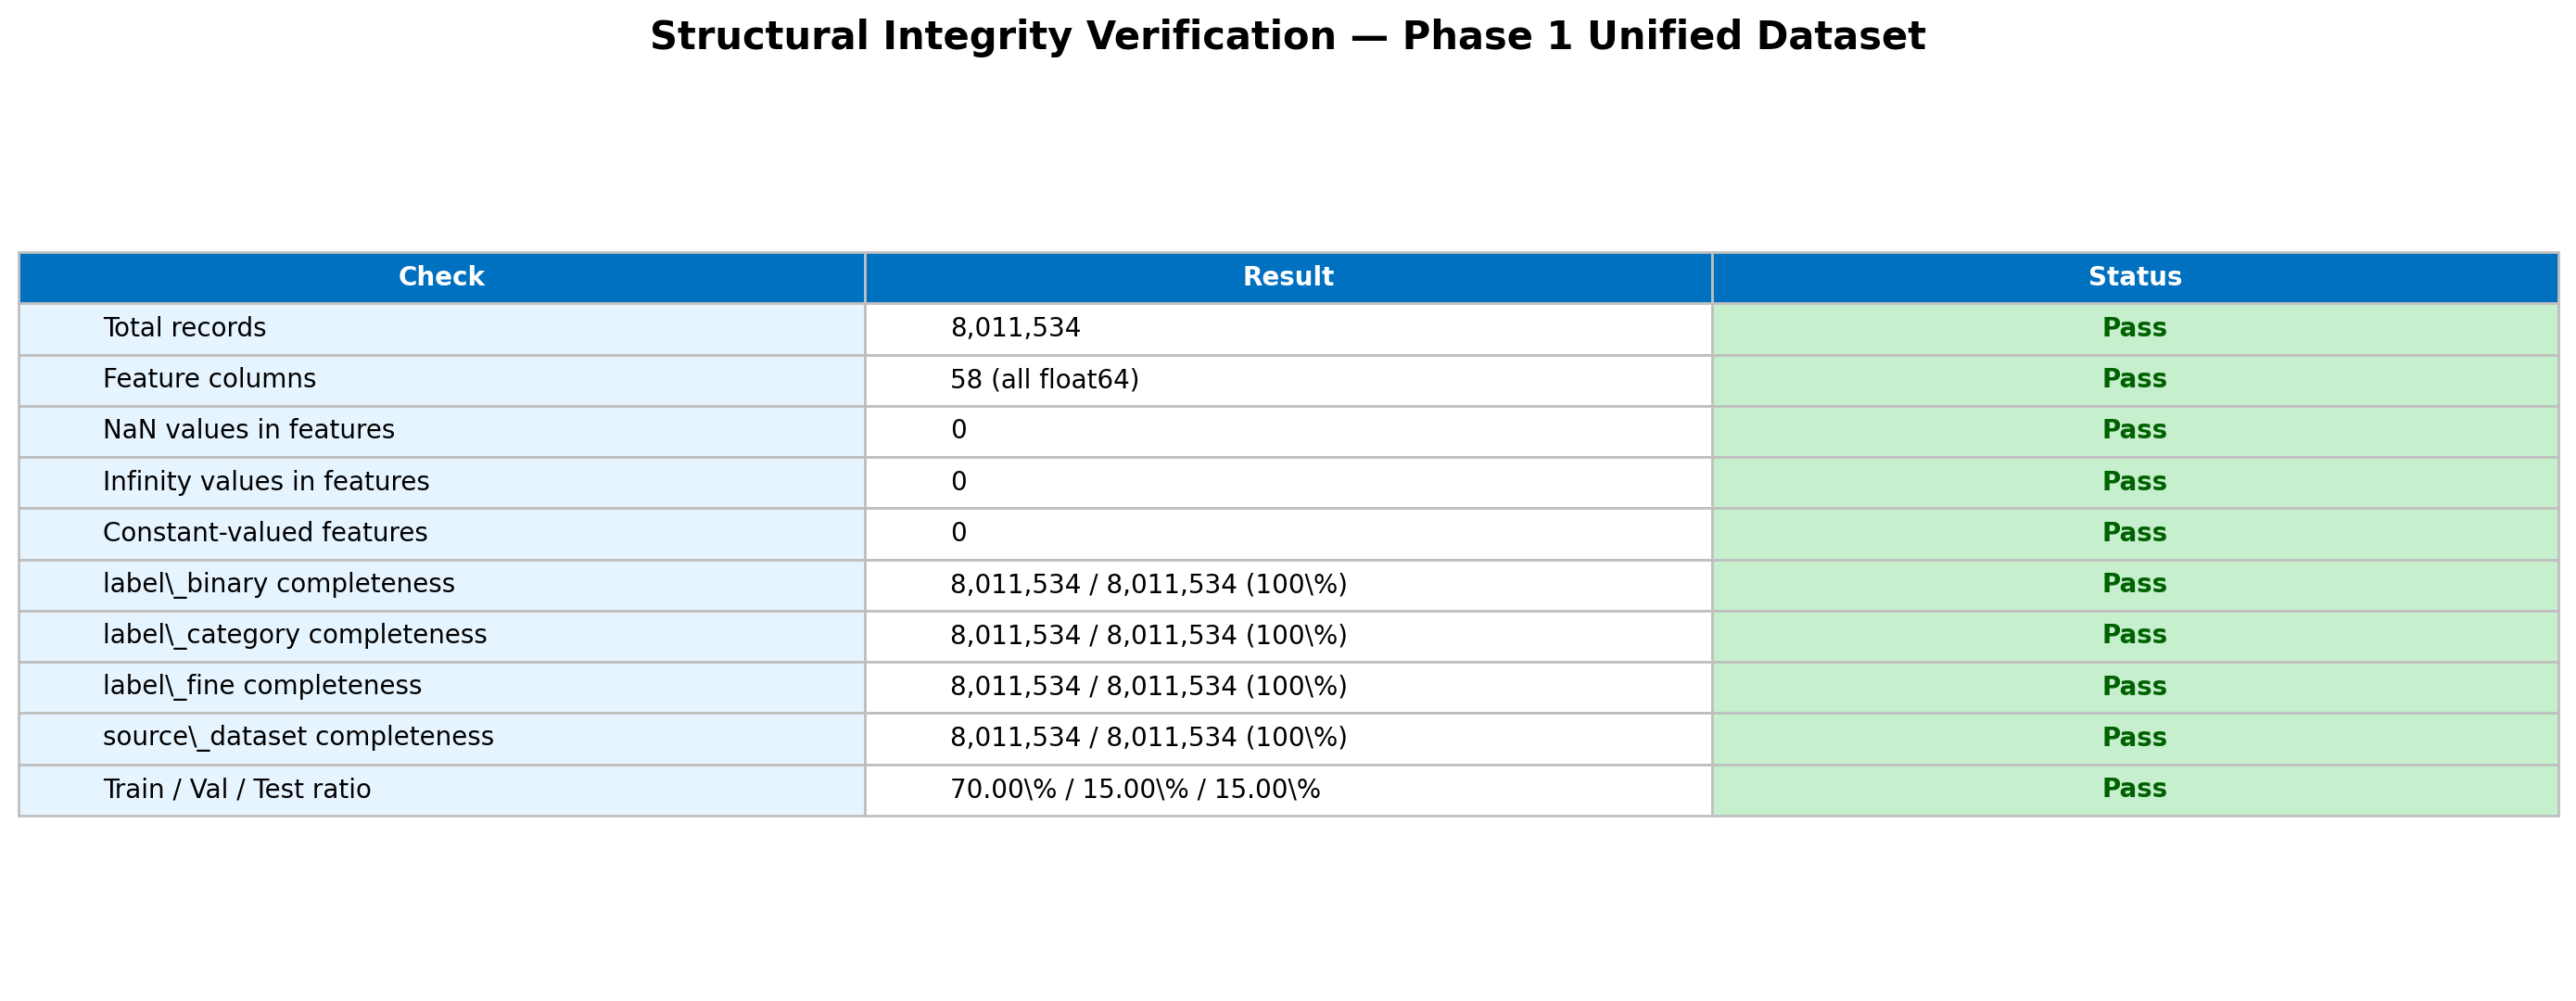
\includegraphics[width=0.9\textwidth]{structural_integrity_check.png}
\caption{Structural integrity verification results. All checks pass, confirming the dataset is well-formed and ready for model training.}
\label{fig:structural-integrity}
\end{figure}

\subsection{Feature Distribution Analysis}
\label{subsec:feature-distributions}

This subsection examines the statistical properties of the 58 scaled features to verify that the standardization process preserved informational content and to characterize the distributional landscape that downstream models will encounter.

\paragraph{Scaling correctness.}
On the training partition, the per-feature means are effectively zero ($\overline{\mu} \approx 1 \times 10^{-8}$) and standard deviations are exactly 1.0, confirming correct \texttt{StandardScaler} behavior. On the validation and test partitions, the maximum absolute mean deviation from zero is 0.0013 and 0.0026 respectively, and the standard deviations remain close to unity. These small deviations are expected and \textit{desirable}: they confirm that no information from the validation/test sets leaked into the scaling parameters.

\paragraph{Distribution shape.}
The majority of features exhibit heavy-tailed, non-Gaussian distributions: 52 of the 58 features have $|\text{skewness}| > 2$ and 51 have kurtosis exceeding 10. This is characteristic of network traffic data, where most flows are short and low-volume but a small fraction of flows (particularly during flood attacks) produce extreme outlier values. The scaled feature range spans from $-13.23$ to $+2{,}368.14$, reflecting these heavy tails. Models must therefore be robust to long-tailed input distributions or employ appropriate techniques (e.g., gradient clipping, robust loss functions).

Figure~\ref{fig:feature-dist-source} shows eight representative features, plotted separately for the two source datasets after scaling. The blue outline corresponds to ``CICIoMT2024'' and the orange outline to ``IoMT-TrafficData''. For each feature, overlapping outlines mean the two sources produce values with similar frequency (similar behaviour), while clearly separated peaks indicate that the feature behaves differently across sources. This figure is useful because it lets us check, at a glance, whether the preprocessing makes the feature values comparable and whether some features carry source-specific patterns that can affect later learning.

\begin{figure}[htbp]
\centering
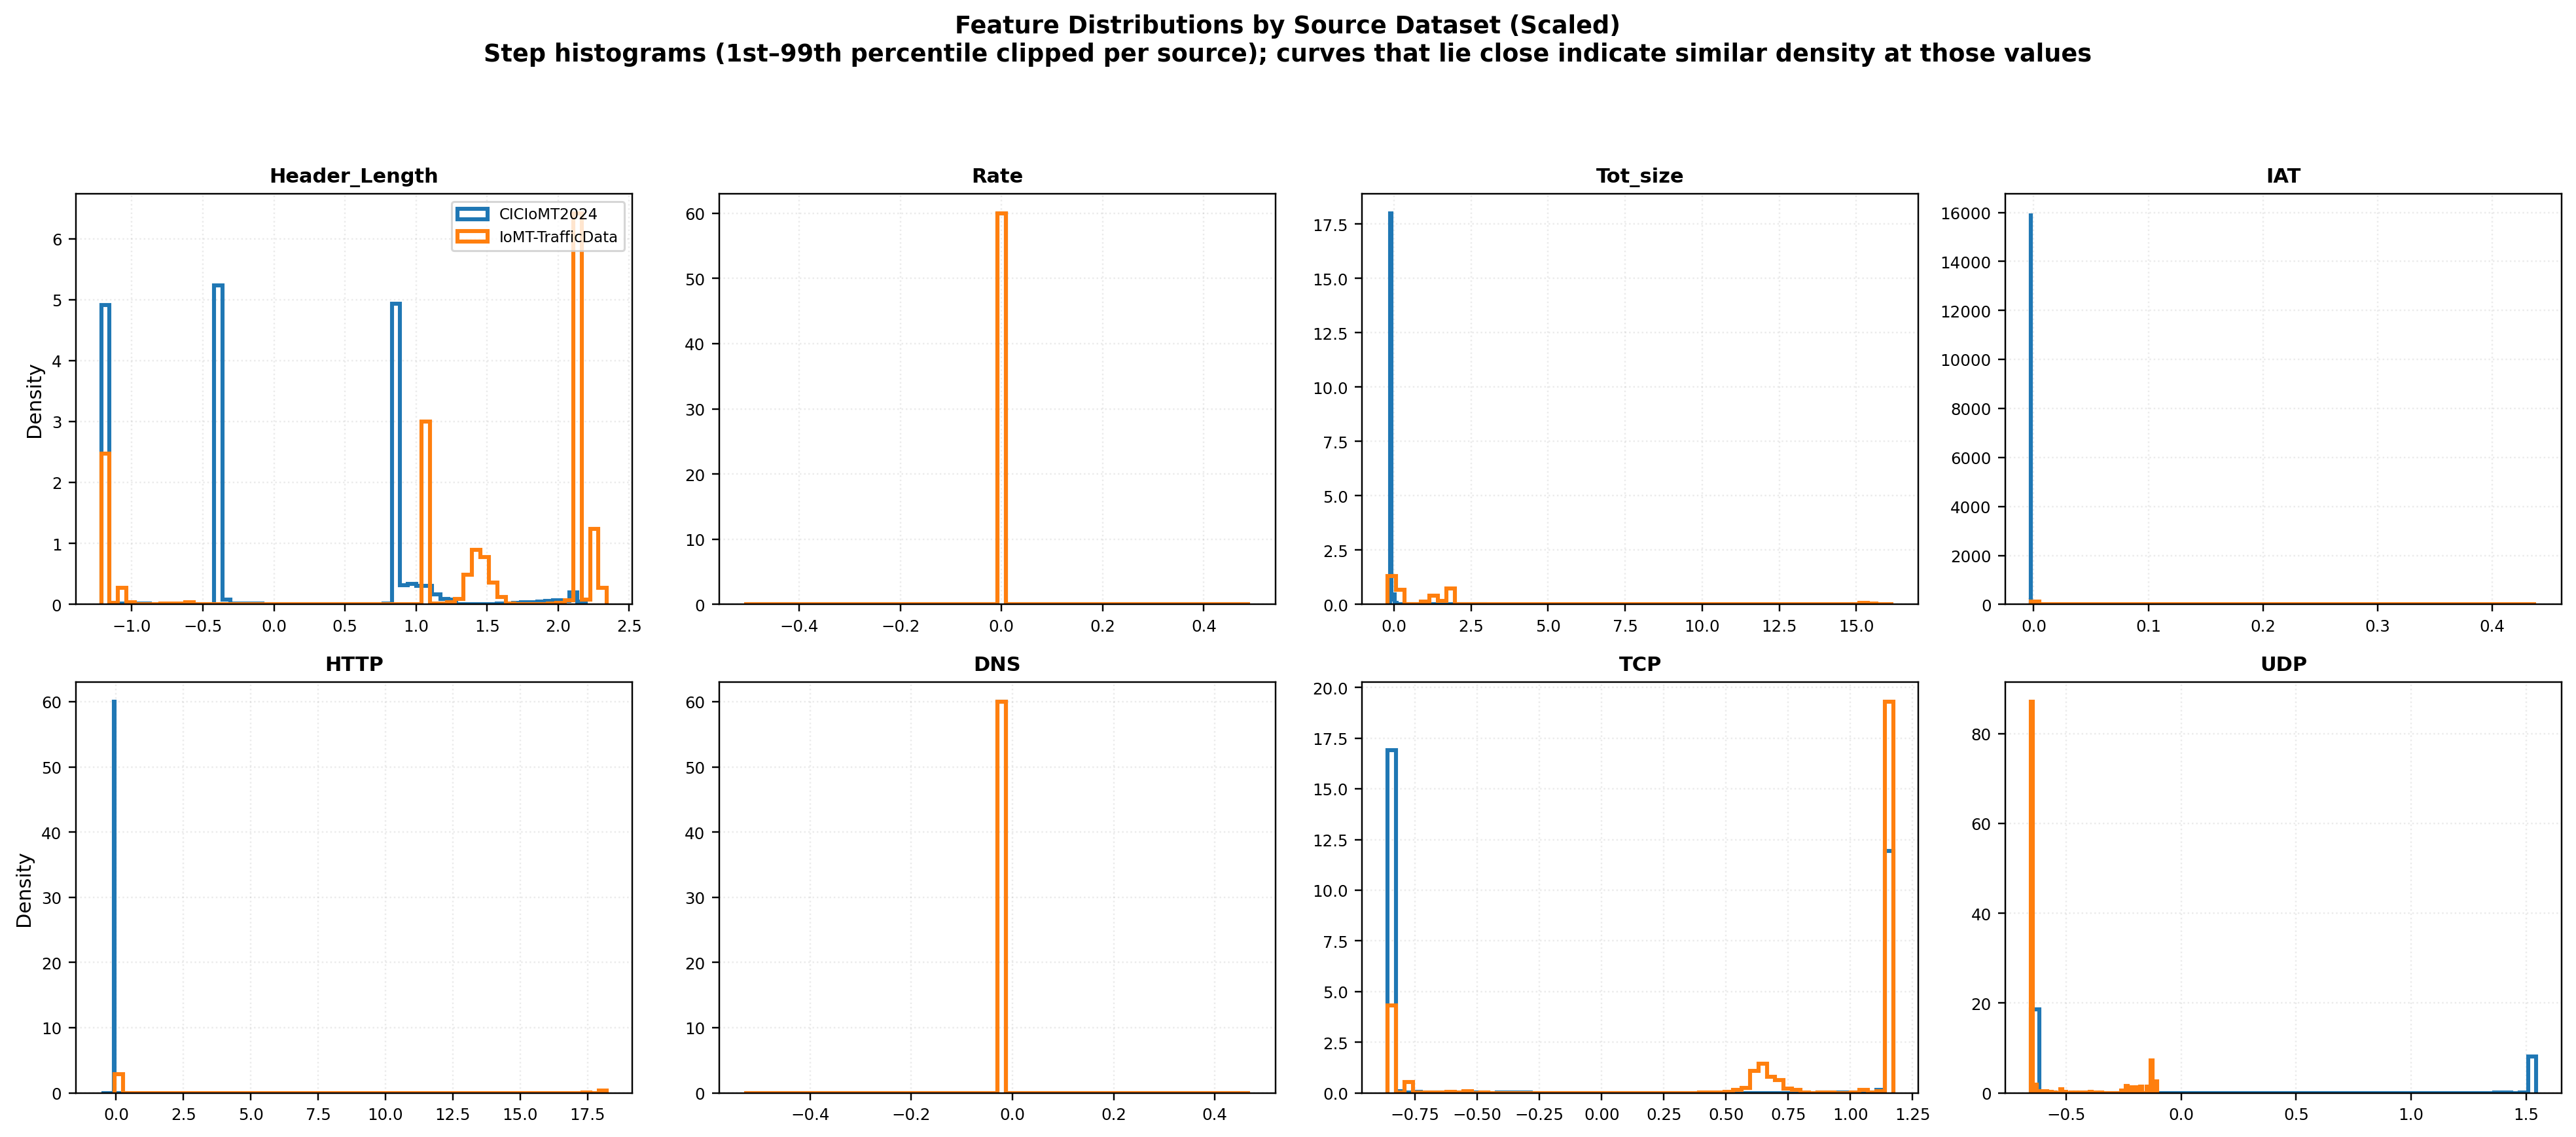
\includegraphics[width=\textwidth]{ch5_feature_distributions_by_source.png}
\caption{Feature distributions after scaling for eight representative features. Blue: CICIoMT2024; orange: IoMT-TrafficData. Overlap suggests similar value frequencies across sources, while separated peaks indicate source-specific behaviour.}
\label{fig:feature-dist-source}
\end{figure}

Figure~\ref{fig:scaling-verification} provides a global view of the scaling quality: per-feature means and standard deviations are plotted for all three partitions. The training set (green) adheres tightly to the theoretical targets of 0 and 1, while the validation and test sets (blue, red) exhibit only minimal deviations, as expected from correctly applied train-only scaling.

\begin{figure}[H]
\centering
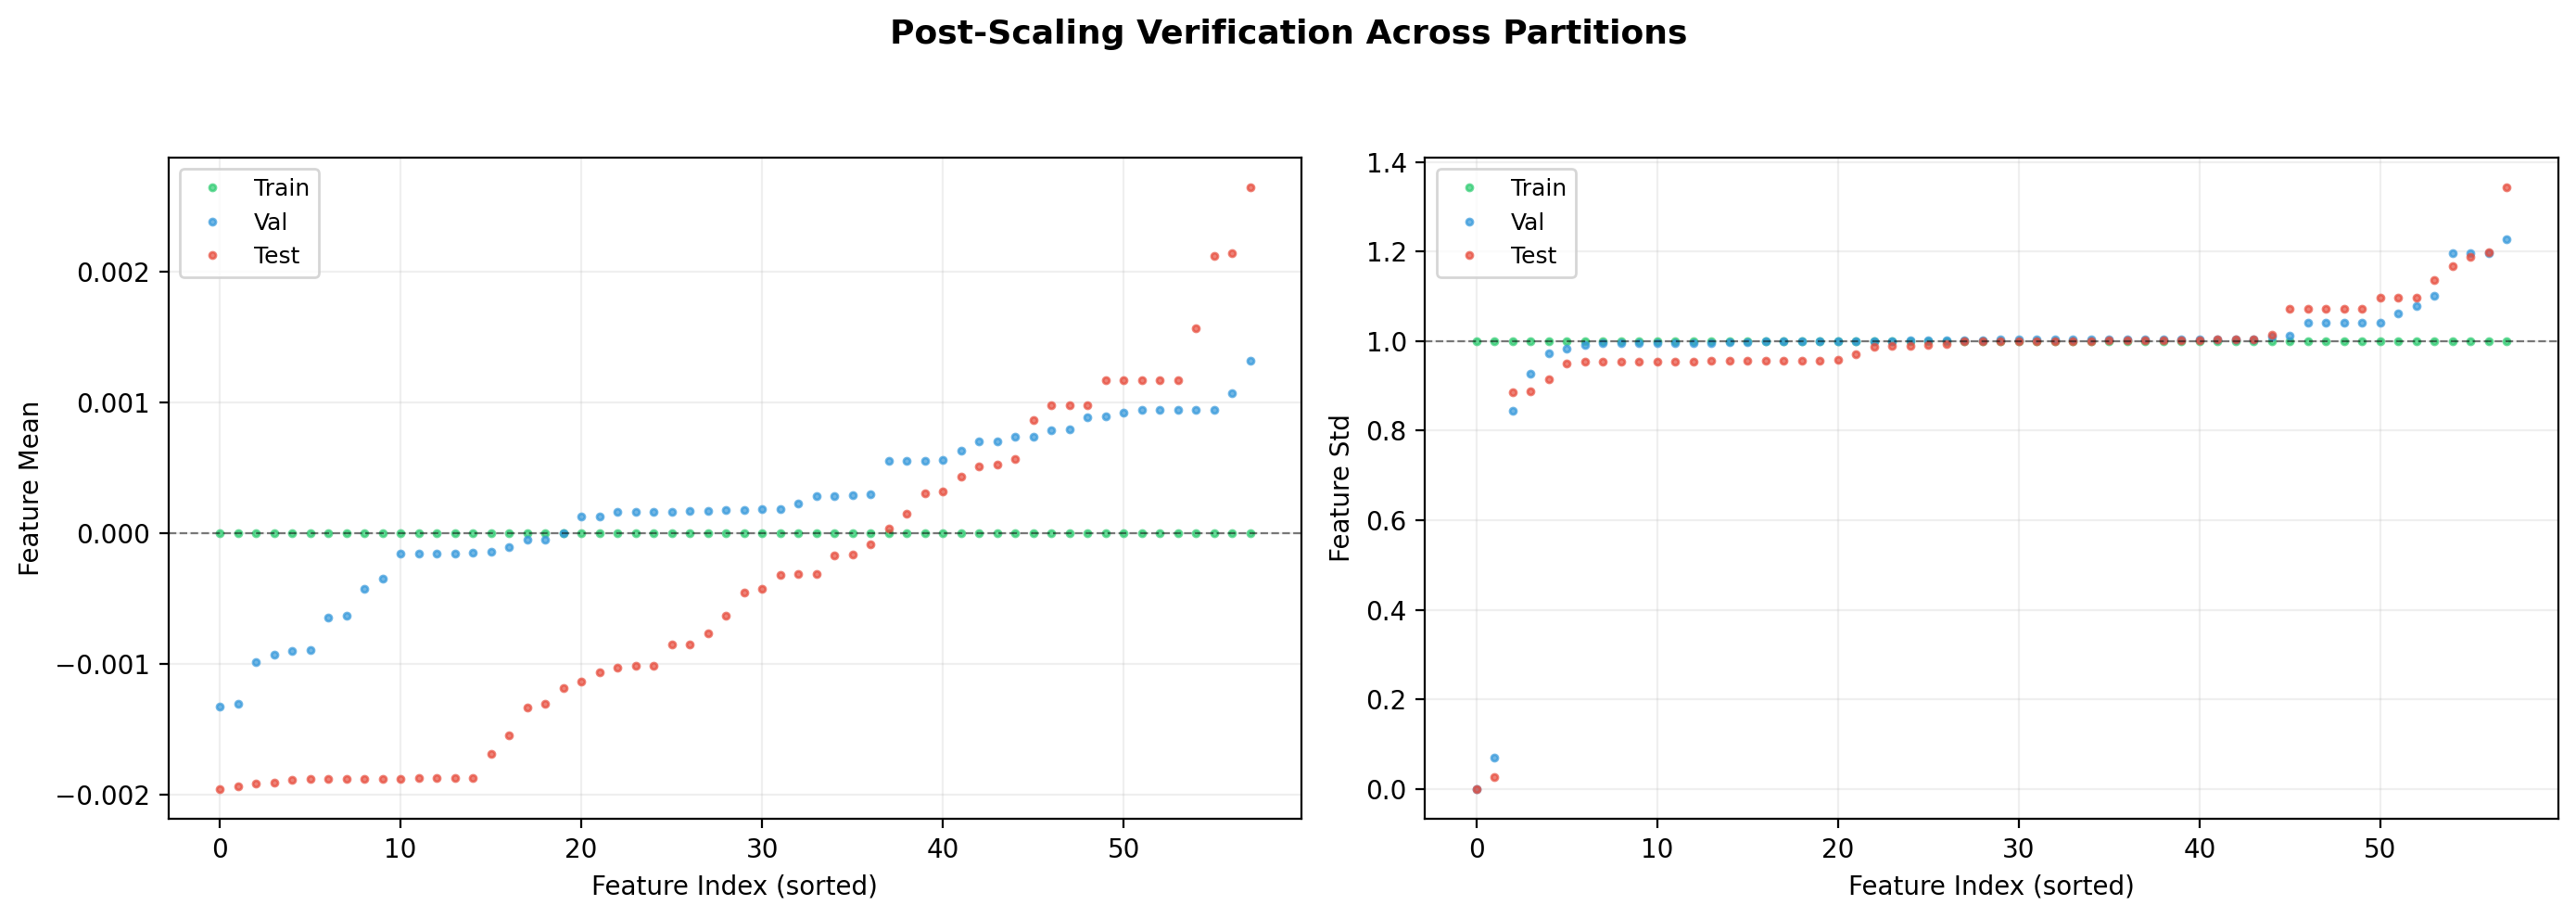
\includegraphics[width=\textwidth]{ch5_scaling_verification.png}
\caption{Post-scaling verification. Left: per-feature means across all three partitions. Right: per-feature standard deviations. The training set matches the theoretical targets exactly; validation/test deviations are minimal, confirming no data leakage.}
\label{fig:scaling-verification}
\end{figure}
\FloatBarrier

\subsection{Class Balance Assessment}
\label{subsec:class-balance}

Class imbalance is a critical consideration for intrusion detection datasets, as it directly affects model training dynamics, evaluation metric interpretation, and operational deployment decisions. This subsection quantifies the imbalance at all three label granularities.

\paragraph{Binary level.}
The dataset is heavily attack-dominated: 7,958,078 records (99.33\%) are labeled \texttt{Attack} and only 53,456 (0.67\%) are \texttt{Benign}. This approximately 149:1 ratio reflects the experimental design of both source datasets, which were constructed to comprehensively capture attack traffic rather than to model realistic benign-to-attack ratios.

\paragraph{Category level.}
Six categories exhibit substantial imbalance, with a maximum-to-minimum ratio of approximately 575:1 (DDoS vs.\ Spoofing). Table~\ref{tab:class-balance} provides the full distribution. The Shannon entropy of the category distribution is 1.209 out of a theoretical maximum of 2.585 (for a uniform 6-class distribution), yielding a normalized entropy of 0.468---indicating moderate concentration. DDoS and DoS together account for 93.83\% of all records, while the remaining four categories collectively represent only 6.17\%.

\begin{table}[H]
\centering
\caption{Category-level class distribution in the final Phase~1 dataset.}
\label{tab:class-balance}
\small
\begin{tabular}{@{}l r r@{}}
\toprule
\textbf{Category} & \textbf{Records} & \textbf{Proportion} \\
\midrule
DDoS & 5,368,292 & 67.01\% \\
DoS & 2,148,477 & 26.82\% \\
MQTT & 385,938 & 4.82\% \\
Benign & 53,456 & 0.67\% \\
Reconnaissance & 46,026 & 0.57\% \\
Spoofing & 9,345 & 0.12\% \\
\midrule
\textbf{Total} & \textbf{8,011,534} & \textbf{100\%} \\
\bottomrule
\end{tabular}
\end{table}

\paragraph{Fine-grained level.}
At the most detailed level, 26 distinct attack types span four orders of magnitude: \texttt{TCP\_IP-DDoS-ICMP} (1,739,060 records) is the most frequent, while \texttt{Recon-Ping\_Sweep} (94 records) is the rarest, yielding an extreme imbalance ratio of approximately 18,500:1. This level of imbalance makes fine-grained classification challenging and motivates the use of class-weighted losses, oversampling, or hierarchical classification strategies in subsequent experiments.

\paragraph{Stratification verification.}
The stratified splitting successfully preserves category proportions across all three partitions. Figure~\ref{fig:class-balance} confirms that per-category percentages are virtually identical in the train, validation, and test sets, ensuring that evaluation metrics reflect genuine model performance rather than partition-level distributional artifacts.

\begin{figure}[htbp]
\centering
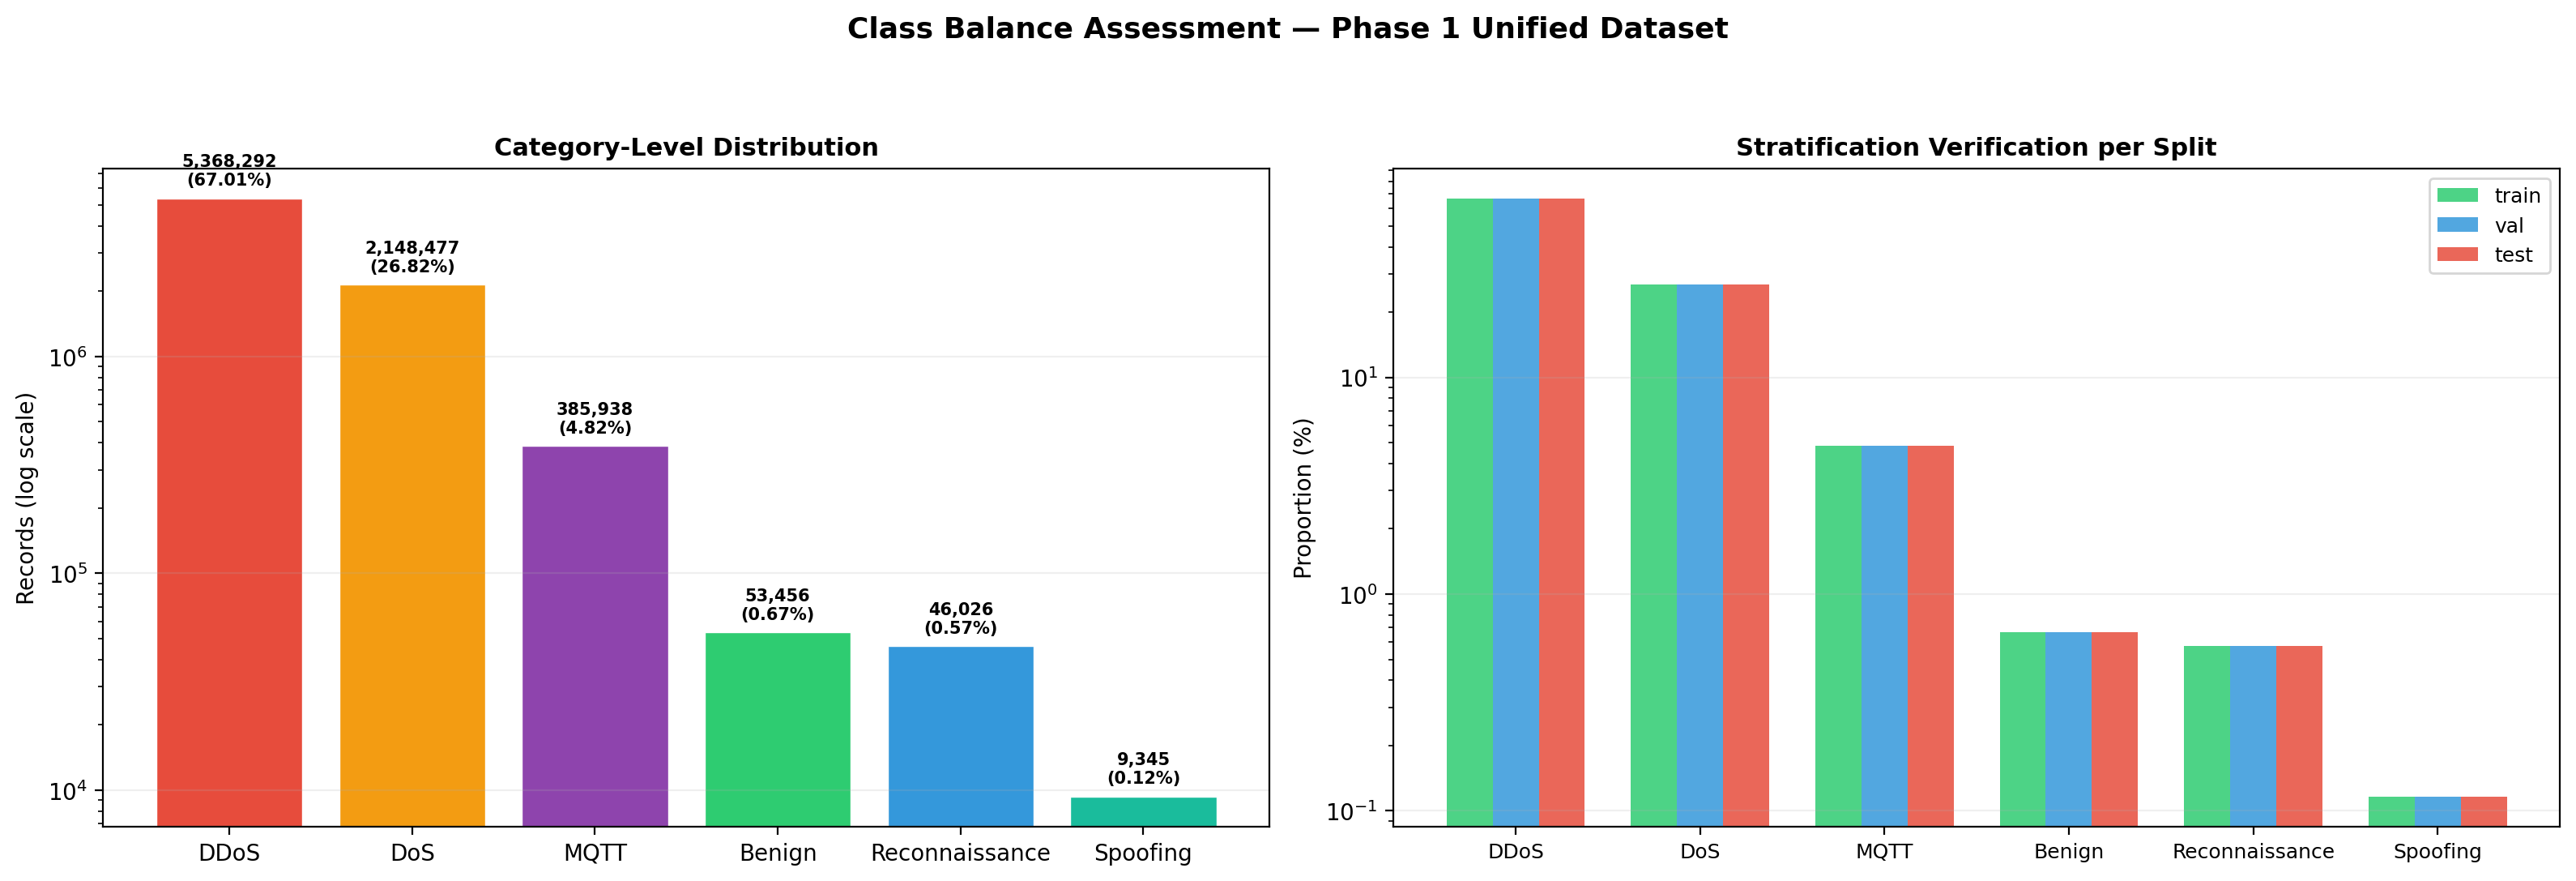
\includegraphics[width=\textwidth]{ch5_class_balance.png}
\caption{Class balance assessment. Left: category-level distribution (log scale) with absolute counts and percentages. Right: per-split category proportions confirming successful stratification.}
\label{fig:class-balance}
\end{figure}

\paragraph{Implications for model training.}
The observed imbalance necessitates careful metric selection: overall accuracy would be misleadingly high due to majority-class dominance. Instead, macro-averaged F1-score and per-class recall will serve as primary evaluation metrics in Section~\ref{sec:model-evaluation}, and class-weighted loss functions will be employed during training to ensure that minority categories (Spoofing, Reconnaissance, Benign) receive adequate gradient signal.

\subsection{Cross-Source Consistency Analysis}
\label{subsec:cross-source}

The unified dataset integrates traffic from two fundamentally different IoMT environments---CICIoMT2024 (a large-scale multi-device testbed) and IoMT-TrafficData (a hospital-oriented testbed). This subsection examines whether source-specific distributional differences are preserved (a desirable property for generalization) versus whether integration introduced artificial artifacts.

\paragraph{Feature-level statistics.}
The two sources exhibit meaningfully different feature-level statistics. CICIoMT2024 records have a mean-of-means of $-0.014$ and a mean-of-standard-deviations of $0.807$ across the 58 features, while IoMT-TrafficData records show a mean-of-means of $0.602$ and a mean-of-standard-deviations of $2.338$. The higher variance in IoMT-TrafficData is expected: as the smaller dataset (2.30\% of records), its records are drawn from a more diverse set of attack methodologies relative to its size, and the scaler was fitted predominantly on CICIoMT2024 traffic.

\paragraph{Category composition.}
The two sources contribute qualitatively different category profiles (see Section~\ref{subsec:label-distributions}). CICIoMT2024 is dominated by DDoS (68.58\%) and DoS (26.84\%), with MQTT, Reconnaissance, Benign, and Spoofing each contributing less than 5\%. IoMT-TrafficData has a more balanced distribution: MQTT (35.68\%), DoS (25.91\%), Reconnaissance (17.85\%), Benign (16.46\%), and Spoofing (4.10\%)---and no DDoS traffic at all. This complementarity is by design and is the core motivation for integration.

\paragraph{Shared fine-grained labels.}
Two fine-grained attack types appear in both datasets: \texttt{Benign} and \texttt{ARP\_Spoofing}. These shared labels enable direct cross-environment comparison for the same attack/traffic type, providing a built-in benchmark for evaluating whether a model can generalize the detection of identical attacks across different network infrastructures.

\paragraph{PCA visualization.}
Figure~\ref{fig:pca-cross-source} is a 2D projection of the unified dataset obtained with PCA. Each point corresponds to one record. The left panel colors points by source dataset (CICIoMT2024 vs. IoMT-TrafficData), while the right panel colors points by attack category. Points that group together indicate records with similar patterns in the reduced feature space; mixing between colours suggests overlap between groups. This figure is useful as a qualitative check: it helps us see whether the sources are represented in a similar feature space (supporting unified learning) and whether attack categories create distinguishable structure that the models can potentially learn.

\begin{figure}[htbp]
\centering
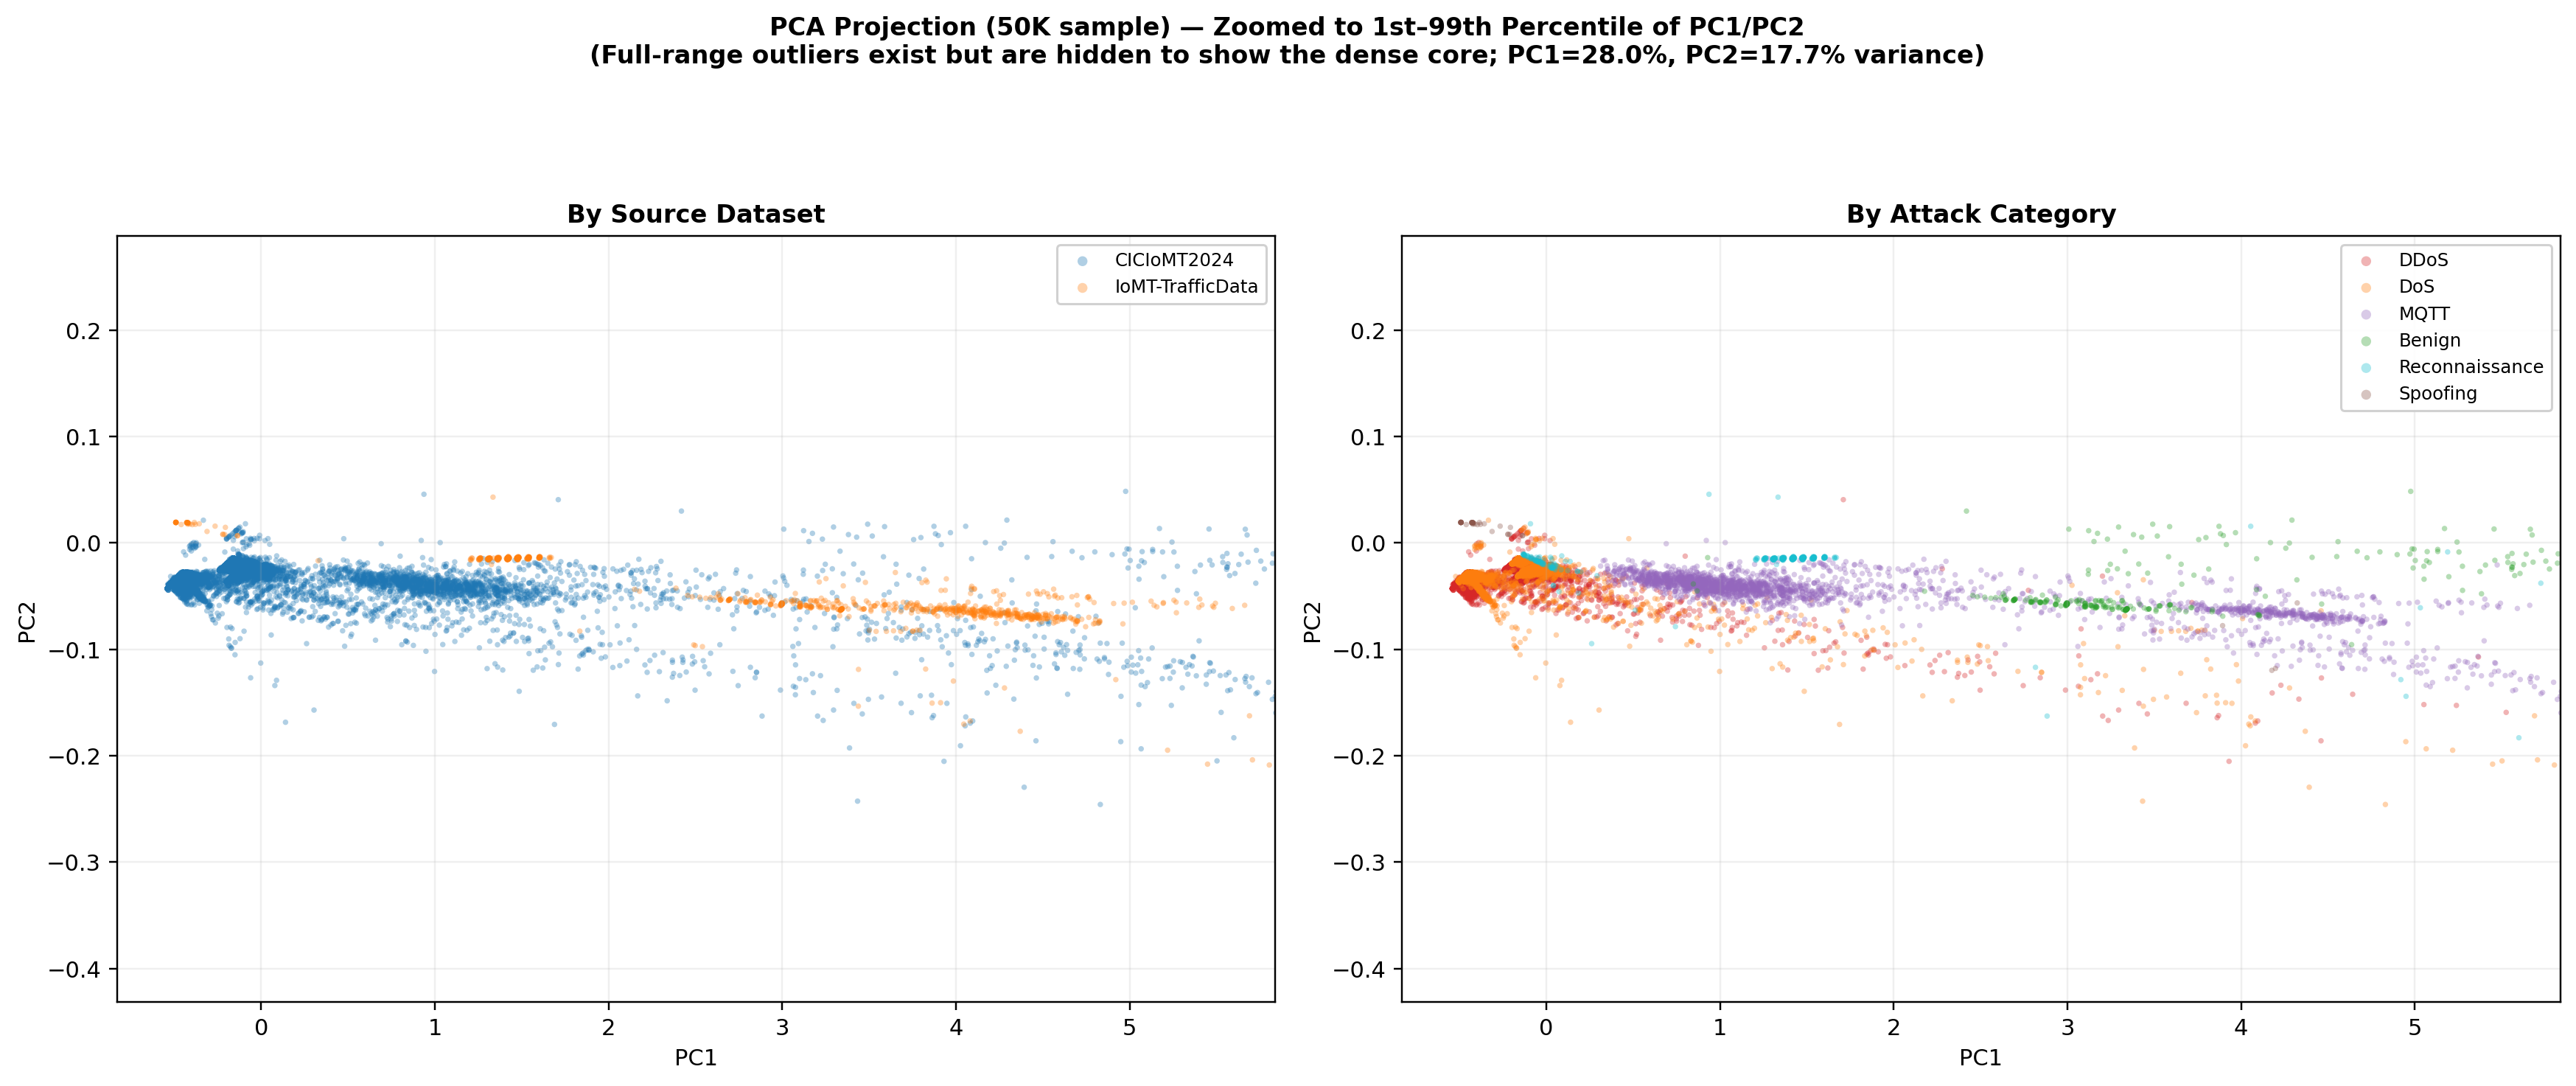
\includegraphics[width=\textwidth]{ch5_pca_cross_source.png}
\caption{PCA projection of a 50K sample from the unified dataset. Left: points colored by source dataset. Right: points colored by attack category. The grouping pattern indicates similarity in the reduced feature space.}
\label{fig:pca-cross-source}
\end{figure}

\paragraph{Assessment summary.}
The cross-source analysis confirms that the integration pipeline successfully preserved the genuine distributional differences between the two IoMT environments without introducing artificial artifacts. The partial overlap in PCA space indicates that models trained on the unified dataset can leverage shared structure across sources while also learning source-specific patterns---precisely the outcome that motivates multi-source integration for improved generalizability.

% ══════════════════════════════════════════════════════════════════════════════
\section{IDS Model Evaluation}
\label{sec:model-evaluation}

This section describes the training, comparison, and evaluation of \gls{ids} models on the unified Phase~1 dataset (dedicated MQTT category mapping, \texttt{StandardScaler} preprocessing as described in Chapter~\ref{ch:execution}). It is placed before the research-question synthesis so that empirical results are available when interpreting integration benefits.

\subsection{Experimental Setup}
\label{subsec:experimental-setup}

The experimental framework is designed to answer the central research question: \emph{does training on the unified multi-source dataset improve generalizability compared to training on each source in isolation?} The protocol follows the methodological recommendations of Lones~\cite{lones2024avoid} and is summarized below.

\paragraph{Algorithm selection.}
Three tree-based classifiers of increasing complexity are evaluated: Decision Tree (DT), Random Forest (RF), and XGBoost. Tree-based models are chosen because they have been shown to outperform deep learning on typical tabular datasets~\cite{grinsztajn2022tree}, and because they natively handle multi-class classification without requiring one-vs-rest wrappers.

\paragraph{Target encoding.}
The six attack categories (\texttt{Benign}, \texttt{DDoS}, \texttt{DoS}, \texttt{MQTT}, \texttt{Reconnaissance}, \texttt{Spoofing}) are encoded as integers 0--5 via \texttt{LabelEncoder}. One-hot encoding of the target variable is deliberately avoided: it would transform the problem into a multi-label setting, which is semantically incorrect for mutually exclusive attack categories. One-hot encoding of features is unnecessary because all 58 input features are already numeric (\texttt{float64}). Tree-based models perform splits per class and do not interpret ordinal relationships among integer target labels, so the choice of LabelEncoder introduces no implicit ordering bias.

A \textbf{global} label mapping (alphabetically sorted across all six categories) is used for all training regimes. This ensures that integer labels are consistent across regimes and that confusion matrices from different experiments are directly comparable---even when a regime's training set does not contain all six classes (e.g., B2 lacks DDoS).

\paragraph{Class imbalance handling.}
The dataset exhibits a 575:1 maximum-to-minimum class ratio (Section~\ref{subsec:class-balance}). For Decision Tree and Random Forest, balanced class weights are applied: each class receives a weight of $n_{\text{samples}} / (n_{\text{classes}} \times n_{\text{class}})$, computed by scikit-learn's \texttt{class\_weight='balanced'} parameter. For XGBoost, equivalent per-sample weights are passed via the \texttt{sample\_weight} argument, as \texttt{scale\_pos\_weight} only applies to binary classification. Synthetic oversampling (e.g., SMOTE) is not used, as the dataset already contains over 8 million records and class weights provide sufficient gradient signal for minority classes.

\paragraph{Training regimes.}
To isolate the effect of dataset integration, three training regimes share the same tuning budget, search space, and evaluation protocol---the only variable is which rows of the training set are used:

\begin{itemize}[nosep]
  \item \textbf{B1 (CIC-only)}: Only rows with \texttt{source\_dataset = CICIoMT2024}.
  \item \textbf{B2 (IoMT-only)}: Only rows with \texttt{source\_dataset = IoMT-TrafficData}.
  \item \textbf{U (Unified)}: The complete training set (both sources).
\end{itemize}

The filtering is applied to the existing stratified splits (train/val/test), preserving the original non-overlapping partition boundaries. This design ensures that any performance difference is attributable solely to the training data composition, not to differences in preprocessing, feature engineering, or evaluation procedure.

\paragraph{Hyperparameter tuning.}
\texttt{RandomizedSearchCV} is used with $n_{\text{iter}}=50$, 3-fold \texttt{StratifiedKFold} cross-validation on the training set, and \texttt{scoring='f1\_macro'}. The Decision Tree search space includes depth, split/leaf thresholds, split criterion, and \texttt{max\_features} (full Cartesian grids are defined as constants in the Phase~2 training module). Random Forest adds \texttt{n\_estimators}, \texttt{max\_samples} (bootstrap row fraction per tree, also acting as a memory cap), and \texttt{class\_weight} modes. XGBoost searches learning rate, boosting rounds, tree depth, \texttt{min\_child\_weight}, row and column subsampling, $\gamma$, and $\ell_1/\ell_2$ penalties; training uses \texttt{tree\_method='hist'} and \texttt{objective='multi:softmax'} with per-sample weights (see the class-imbalance paragraph under this subsection). Each regime receives the same iteration budget for fair comparison~\cite{lones2024avoid}.

\paragraph{Feasibility of ensemble tuning on large partitions.}
Full \texttt{RandomizedSearchCV} with wide search spaces over hundreds of thousands of training rows and hundreds of trees per candidate is computationally heavy on a single workstation. For Random Forest and XGBoost only, hyperparameter search is therefore performed on a \emph{stratified random subsample} of 300{,}000 training rows whenever the regime's training partition exceeds that size (B1 and U); B2 remains below this threshold and uses the full IoMT-only training set. The best hyperparameter vector from this search is then used to train a final model on the \emph{complete} training partition before the locked test-set evaluation. The held-out test set is still touched only once for reporting; only the inner cross-validation for search uses the subsample. This two-stage procedure is a standard pragmatic compromise in large-scale tabular learning~\cite{lones2024avoid} and keeps the methodology aligned with the Decision Tree protocol aside from this explicit feasibility constraint.

\paragraph{Evaluation protocol.}
Following the ``test set once'' principle (\S4.3 of~\cite{lones2024avoid}), hyperparameters are tuned exclusively on the validation set. The test set is evaluated only once per model to report final metrics, after all tuning decisions are locked. The evaluation matrix covers three test slices per model:

\begin{itemize}[nosep]
  \item \textbf{In-domain}: The test slice matching the training source (e.g., B1 $\to$ CIC test slice).
  \item \textbf{Cross-domain}: The test slice from the \emph{other} source (e.g., B1 $\to$ IoMT test slice).
  \item \textbf{Full}: The complete unified test set.
\end{itemize}

\paragraph{Metrics.}
Overall accuracy is reported only for completeness; it is \textbf{not} used as the primary metric due to severe class imbalance. The primary metric is \textbf{macro-averaged F1-score}, which gives equal weight to each class regardless of its frequency. Weighted F1-score, per-class precision, recall, and F1-score, and normalized confusion matrices are also reported to provide a complete picture. For pairwise model comparison, McNemar's test is applied to the test-set predictions.

\subsection{Decision Tree Classifier}
\label{subsec:decision-tree}

The Decision Tree (DT) classifier serves as the first model in the progressive-complexity sequence (DT $\to$ RF $\to$ XGBoost). Two stages are evaluated per regime: a \emph{baseline} DT with default scikit-learn hyperparameters (only \texttt{class\_weight} set to balanced), and a \emph{tuned} DT with the best hyperparameters from \texttt{RandomizedSearchCV}.

\subsubsection{Baseline Results}

Table~\ref{tab:dt-baseline} reports baseline DT performance across all regime-slice combinations.

\begin{table}[H]
\centering
\caption{Baseline Decision Tree (default hyperparameters) evaluation matrix.}
\label{tab:dt-baseline}
\small
\begin{tabular}{@{}l l c c c@{}}
\toprule
\textbf{Regime} & \textbf{Test slice} & \textbf{Macro-F1} & \textbf{Weighted-F1} & \textbf{Accuracy} \\
\midrule
B1 (CIC-only) & CIC (in-domain)  & 0.9119 & 0.8667 & 0.8668 \\
B1 (CIC-only) & IoMT (cross)     & 0.2256 & 0.3849 & 0.3816 \\
B1 (CIC-only) & Full             & 0.6683 & 0.8542 & 0.8556 \\
\midrule
B2 (IoMT-only) & IoMT (in-domain) & 0.8332 & 0.9998 & 0.9998 \\
B2 (IoMT-only) & CIC (cross)      & 0.0527 & 0.0513 & 0.0617 \\
B2 (IoMT-only) & Full             & 0.3315 & 0.0661 & 0.0833 \\
\midrule
U (Unified)    & CIC              & 0.9143 & 0.8667 & 0.8668 \\
U (Unified)    & IoMT             & 0.8329 & 0.9994 & 0.9993 \\
U (Unified)    & Full             & \textbf{0.9366} & 0.8697 & 0.8699 \\
\bottomrule
\end{tabular}
\end{table}
\FloatBarrier

\subsubsection{Tuned Results}

Table~\ref{tab:dt-tuned} reports the tuned DT results. The best hyperparameters per regime are listed in Table~\ref{tab:dt-best-params}.

\begin{table}[H]
\centering
\caption{Tuned Decision Tree evaluation matrix.}
\label{tab:dt-tuned}
\small
\begin{tabular}{@{}l l c c c@{}}
\toprule
\textbf{Regime} & \textbf{Test slice} & \textbf{Macro-F1} & \textbf{Weighted-F1} & \textbf{Accuracy} \\
\midrule
Tuned B1 & CIC (in-domain)  & 0.9226 & 0.8889 & 0.8853 \\
Tuned B1 & IoMT (cross)     & 0.2474 & 0.3923 & 0.3892 \\
Tuned B1 & Full             & 0.6959 & 0.8769 & 0.8738 \\
\midrule
Tuned B2 & IoMT (in-domain) & 0.8332 & 0.9999 & 0.9999 \\
Tuned B2 & CIC (cross)      & 0.0523 & 0.0619 & 0.0570 \\
Tuned B2 & Full             & 0.3284 & 0.0756 & 0.0787 \\
\midrule
Tuned U  & CIC              & 0.9262 & 0.8899 & 0.8863 \\
Tuned U  & IoMT             & 0.8325 & 0.9990 & 0.9990 \\
Tuned U  & Full             & \textbf{0.9480} & 0.8923 & 0.8889 \\
\bottomrule
\end{tabular}
\end{table}
\FloatBarrier

\paragraph{Note on Macro-F1 interpretation (Table~\ref{tab:dt-tuned}).}
For the Tuned U result on the IoMT slice, the reported Macro-F1 ($0.8325$) is computed over the global six-class label space for consistency across all slices. Because the IoMT slice contains no true DDoS samples (support $=0$), the DDoS class contributes an F1-score of $0$ to the global macro average. If Macro-F1 is computed over present classes only (Benign, DoS, MQTT, Reconnaissance, Spoofing), the value is $0.9990$. Weighted-F1 and accuracy remain $0.9990$ because they are support-weighted and are therefore not penalized by an absent class.

\begin{table}[H]
\centering
\caption{Best hyperparameters per regime (Decision Tree, 50-iteration RandomizedSearchCV).}
\label{tab:dt-best-params}
\small
\begin{tabular}{@{}l c c c c c c@{}}
\toprule
\textbf{Regime} & \textbf{criterion} & \textbf{max\_depth} & \textbf{min\_split} & \textbf{min\_leaf} & \textbf{max\_feat.} & \textbf{CV F1m} \\
\midrule
B1 (CIC-only)  & entropy & 15   & 2 & 2 & None & 0.9232 \\
B2 (IoMT-only) & entropy & 10   & 2 & 1 & None & 0.9998 \\
U (Unified)    & entropy & 15   & 2 & 2 & None & 0.9469 \\
\bottomrule
\end{tabular}
\end{table}

\subsubsection{Cross-Domain Analysis}

The cross-domain evaluation reveals the generalization gap that motivates multi-source integration. When a model trained on only one source (B1 or B2) is evaluated on the other source's test data, performance is expected to degrade---especially for attack categories absent from the training data (e.g., B2 has never seen DDoS traffic).

Figure~\ref{fig:dt-confusion-unified} shows the confusion matrix for the tuned unified DT on the full test set. Figure~\ref{fig:dt-cm-xd} presents the cross-domain confusion matrices that illustrate misclassification patterns when models encounter unseen attack categories.

\begin{figure}[H]
\centering
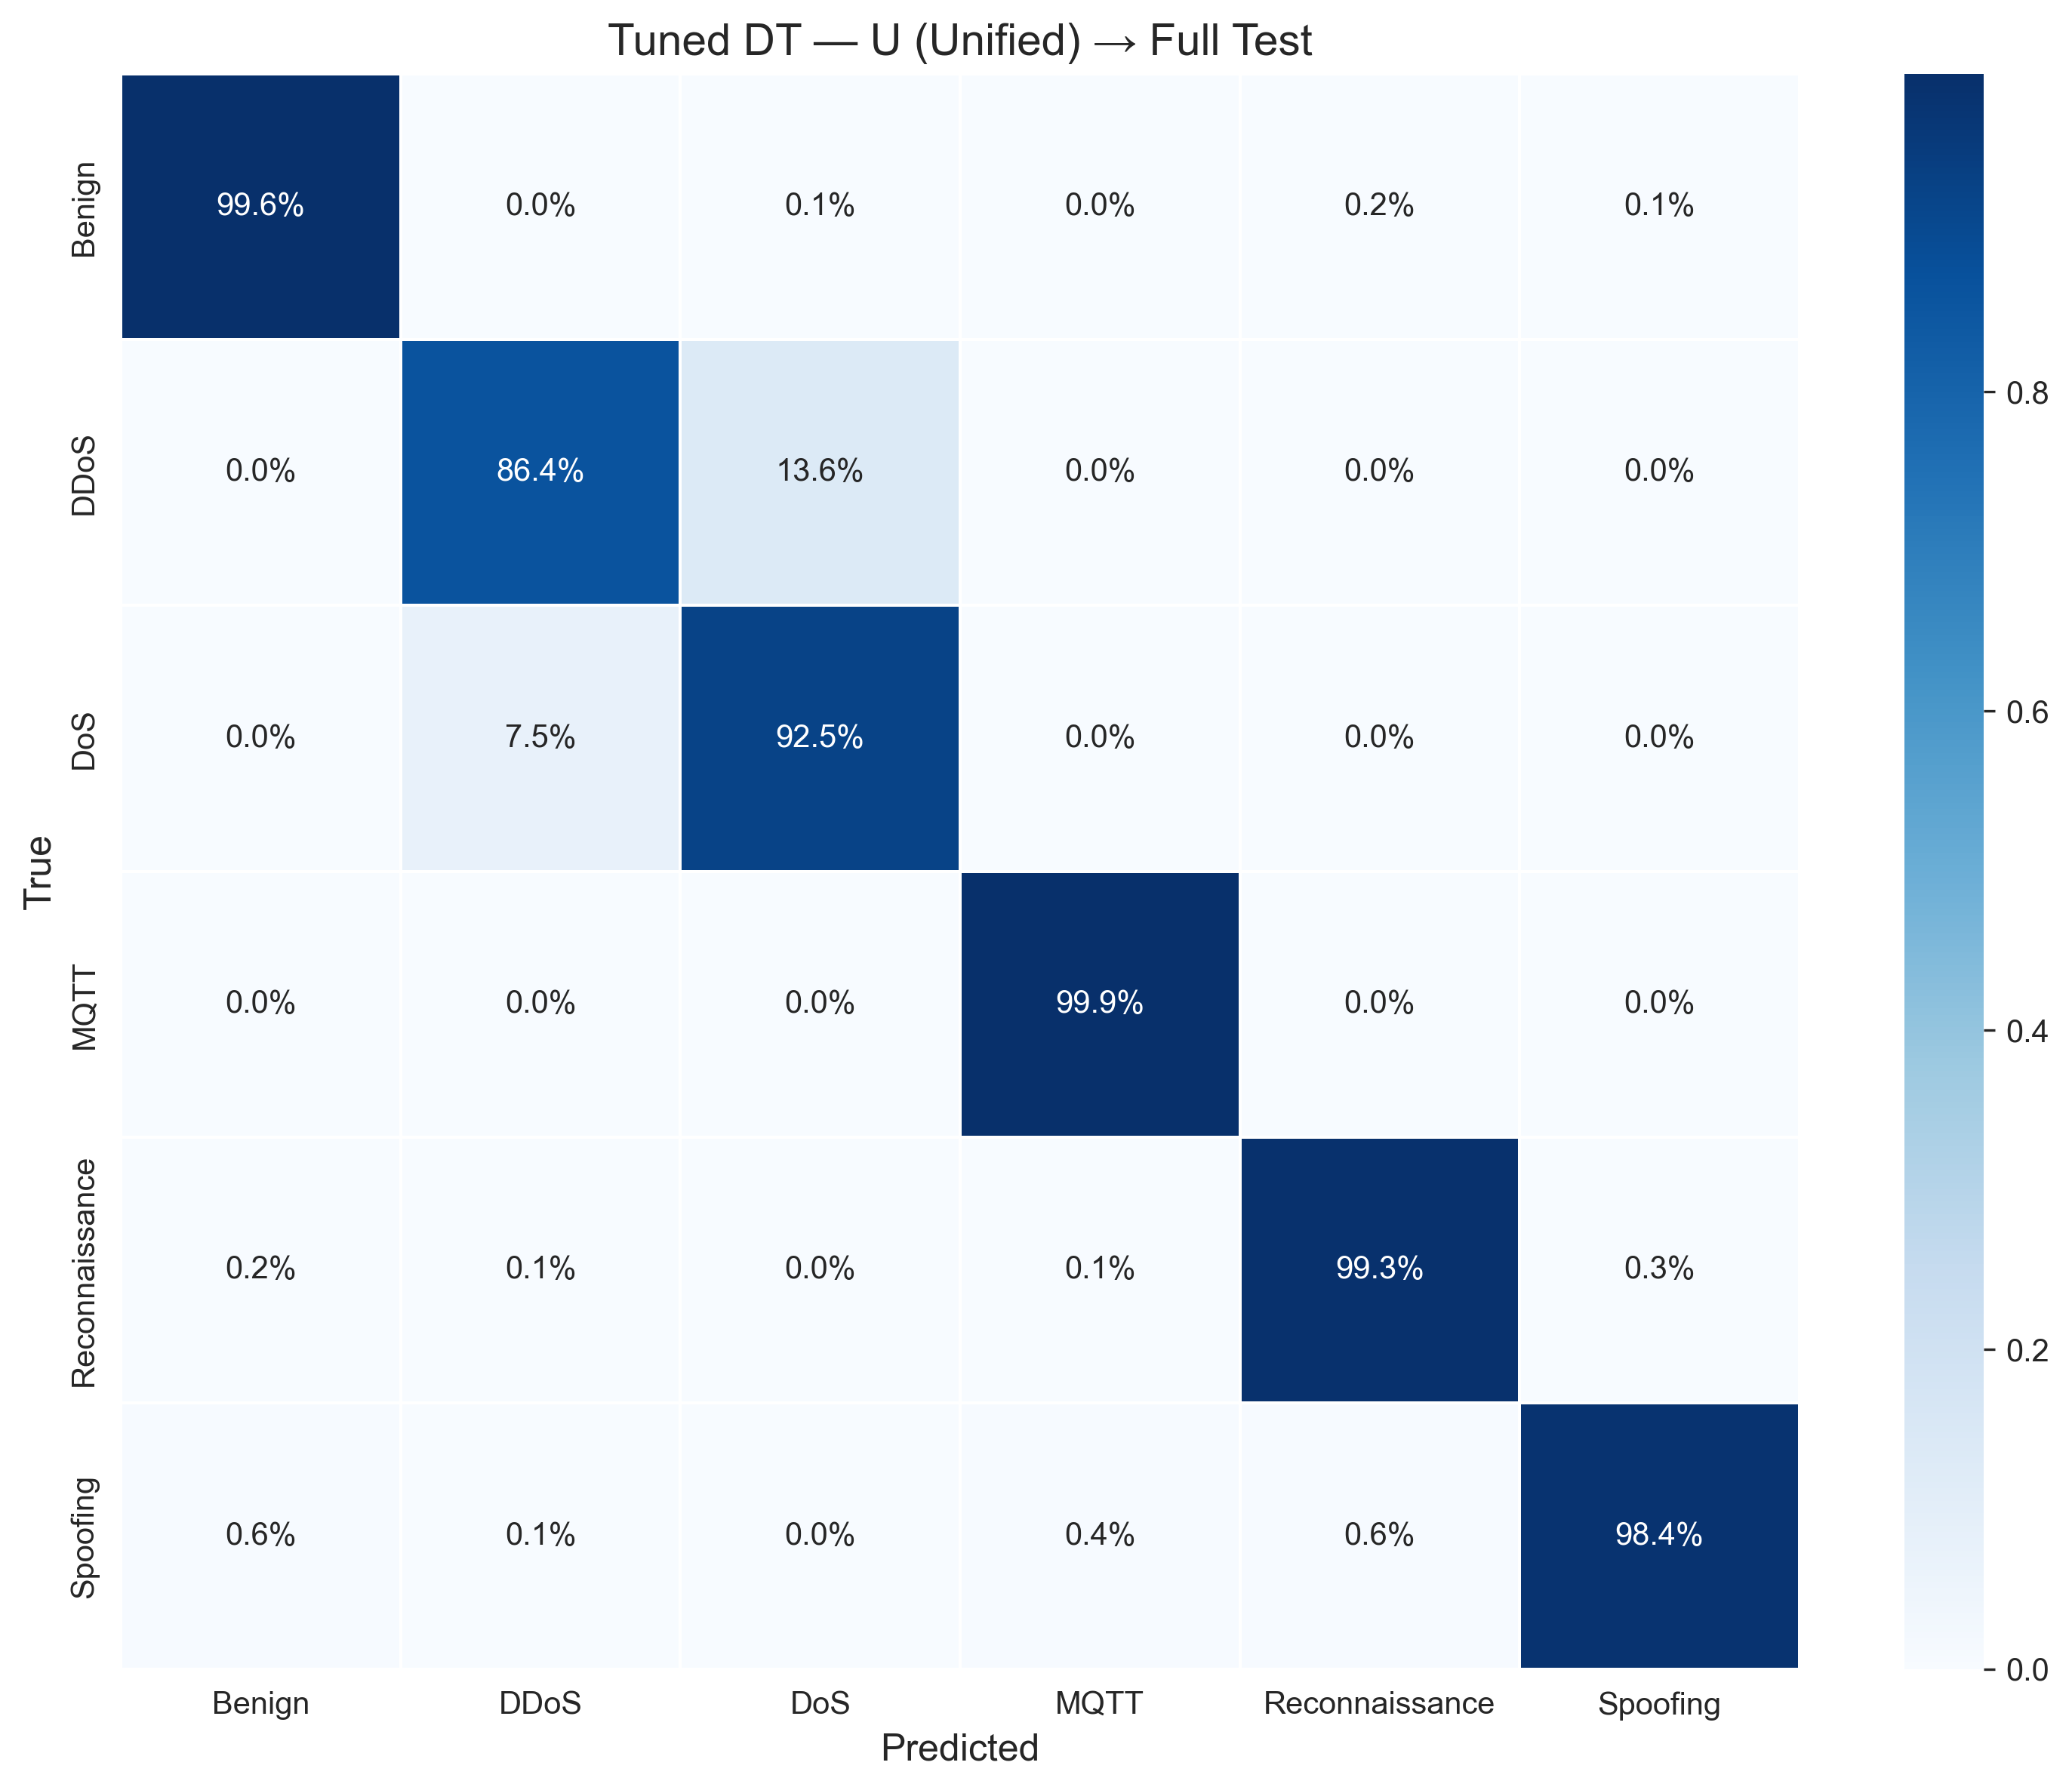
\includegraphics[width=0.75\textwidth]{ch5_dt_cm_u_full.png}
\caption{Normalized confusion matrix --- Tuned DT (Unified) on the full test set.}
\label{fig:dt-confusion-unified}
\end{figure}

\begin{figure}[H]
\centering
\begin{subfigure}[b]{0.48\textwidth}
  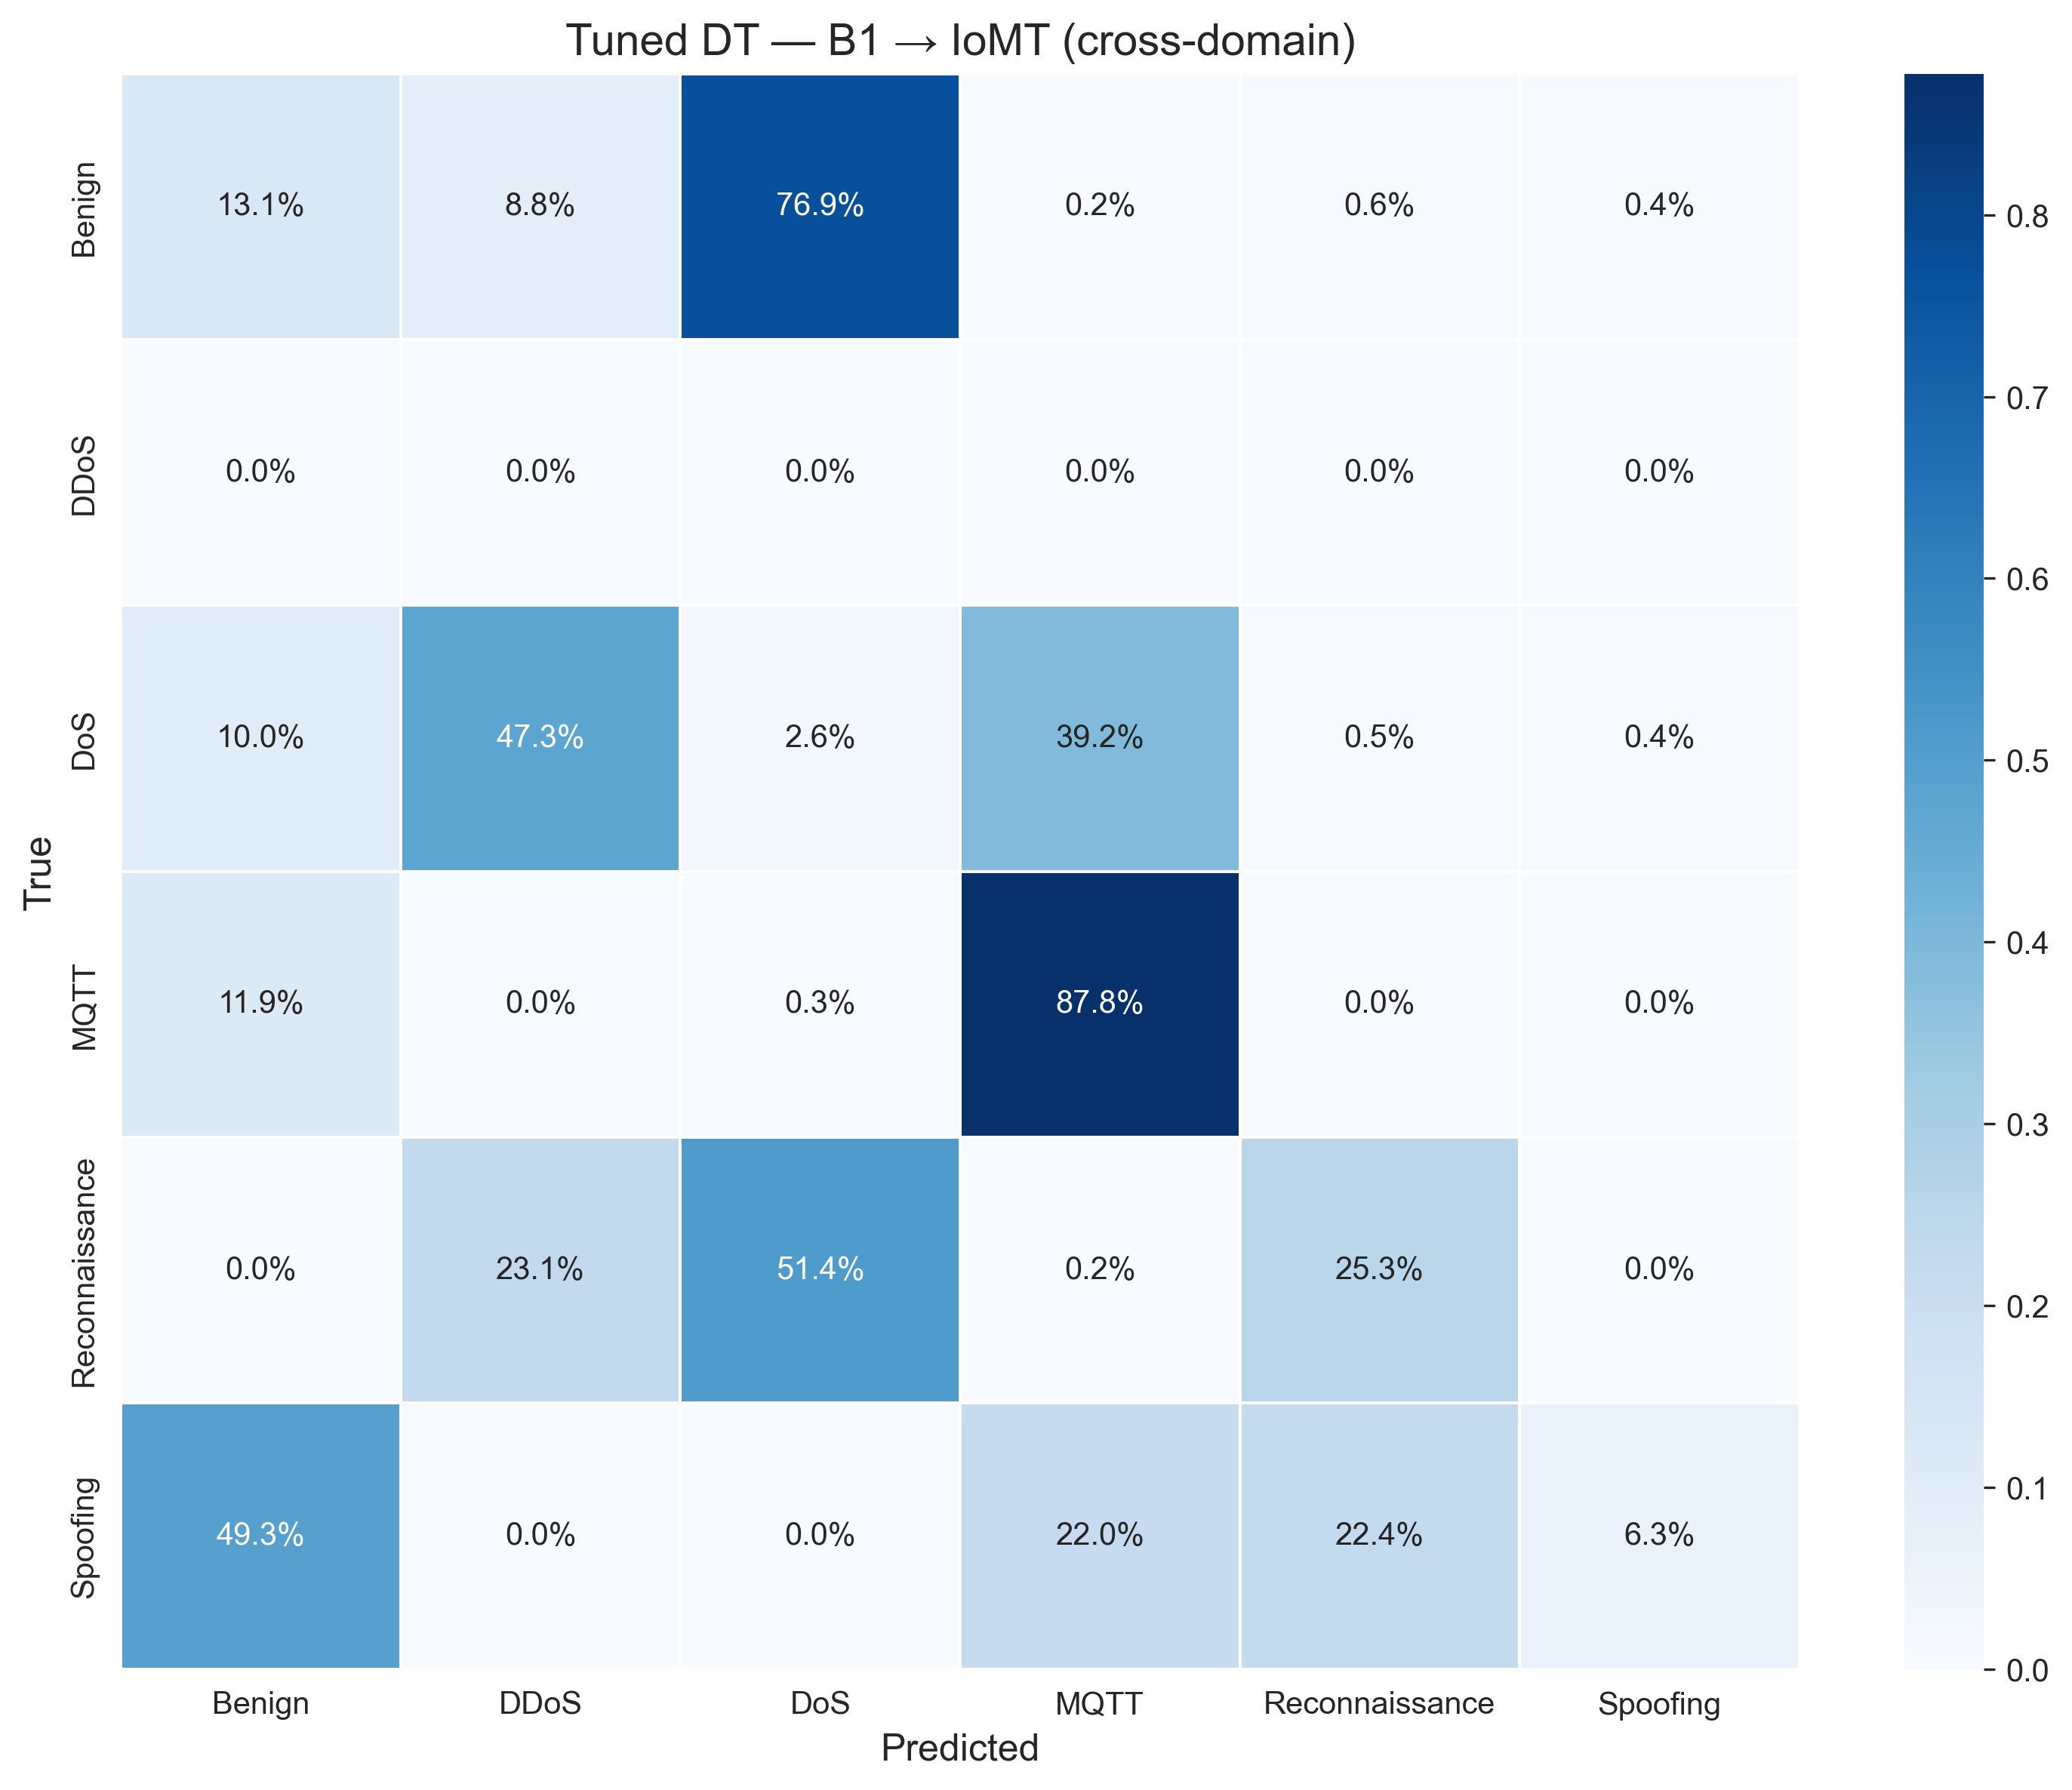
\includegraphics[width=\textwidth]{ch5_dt_cm_b1_xd_iomt.png}
  \caption{B1 (CIC-only) $\to$ IoMT test}
\end{subfigure}
\hfill
\begin{subfigure}[b]{0.48\textwidth}
  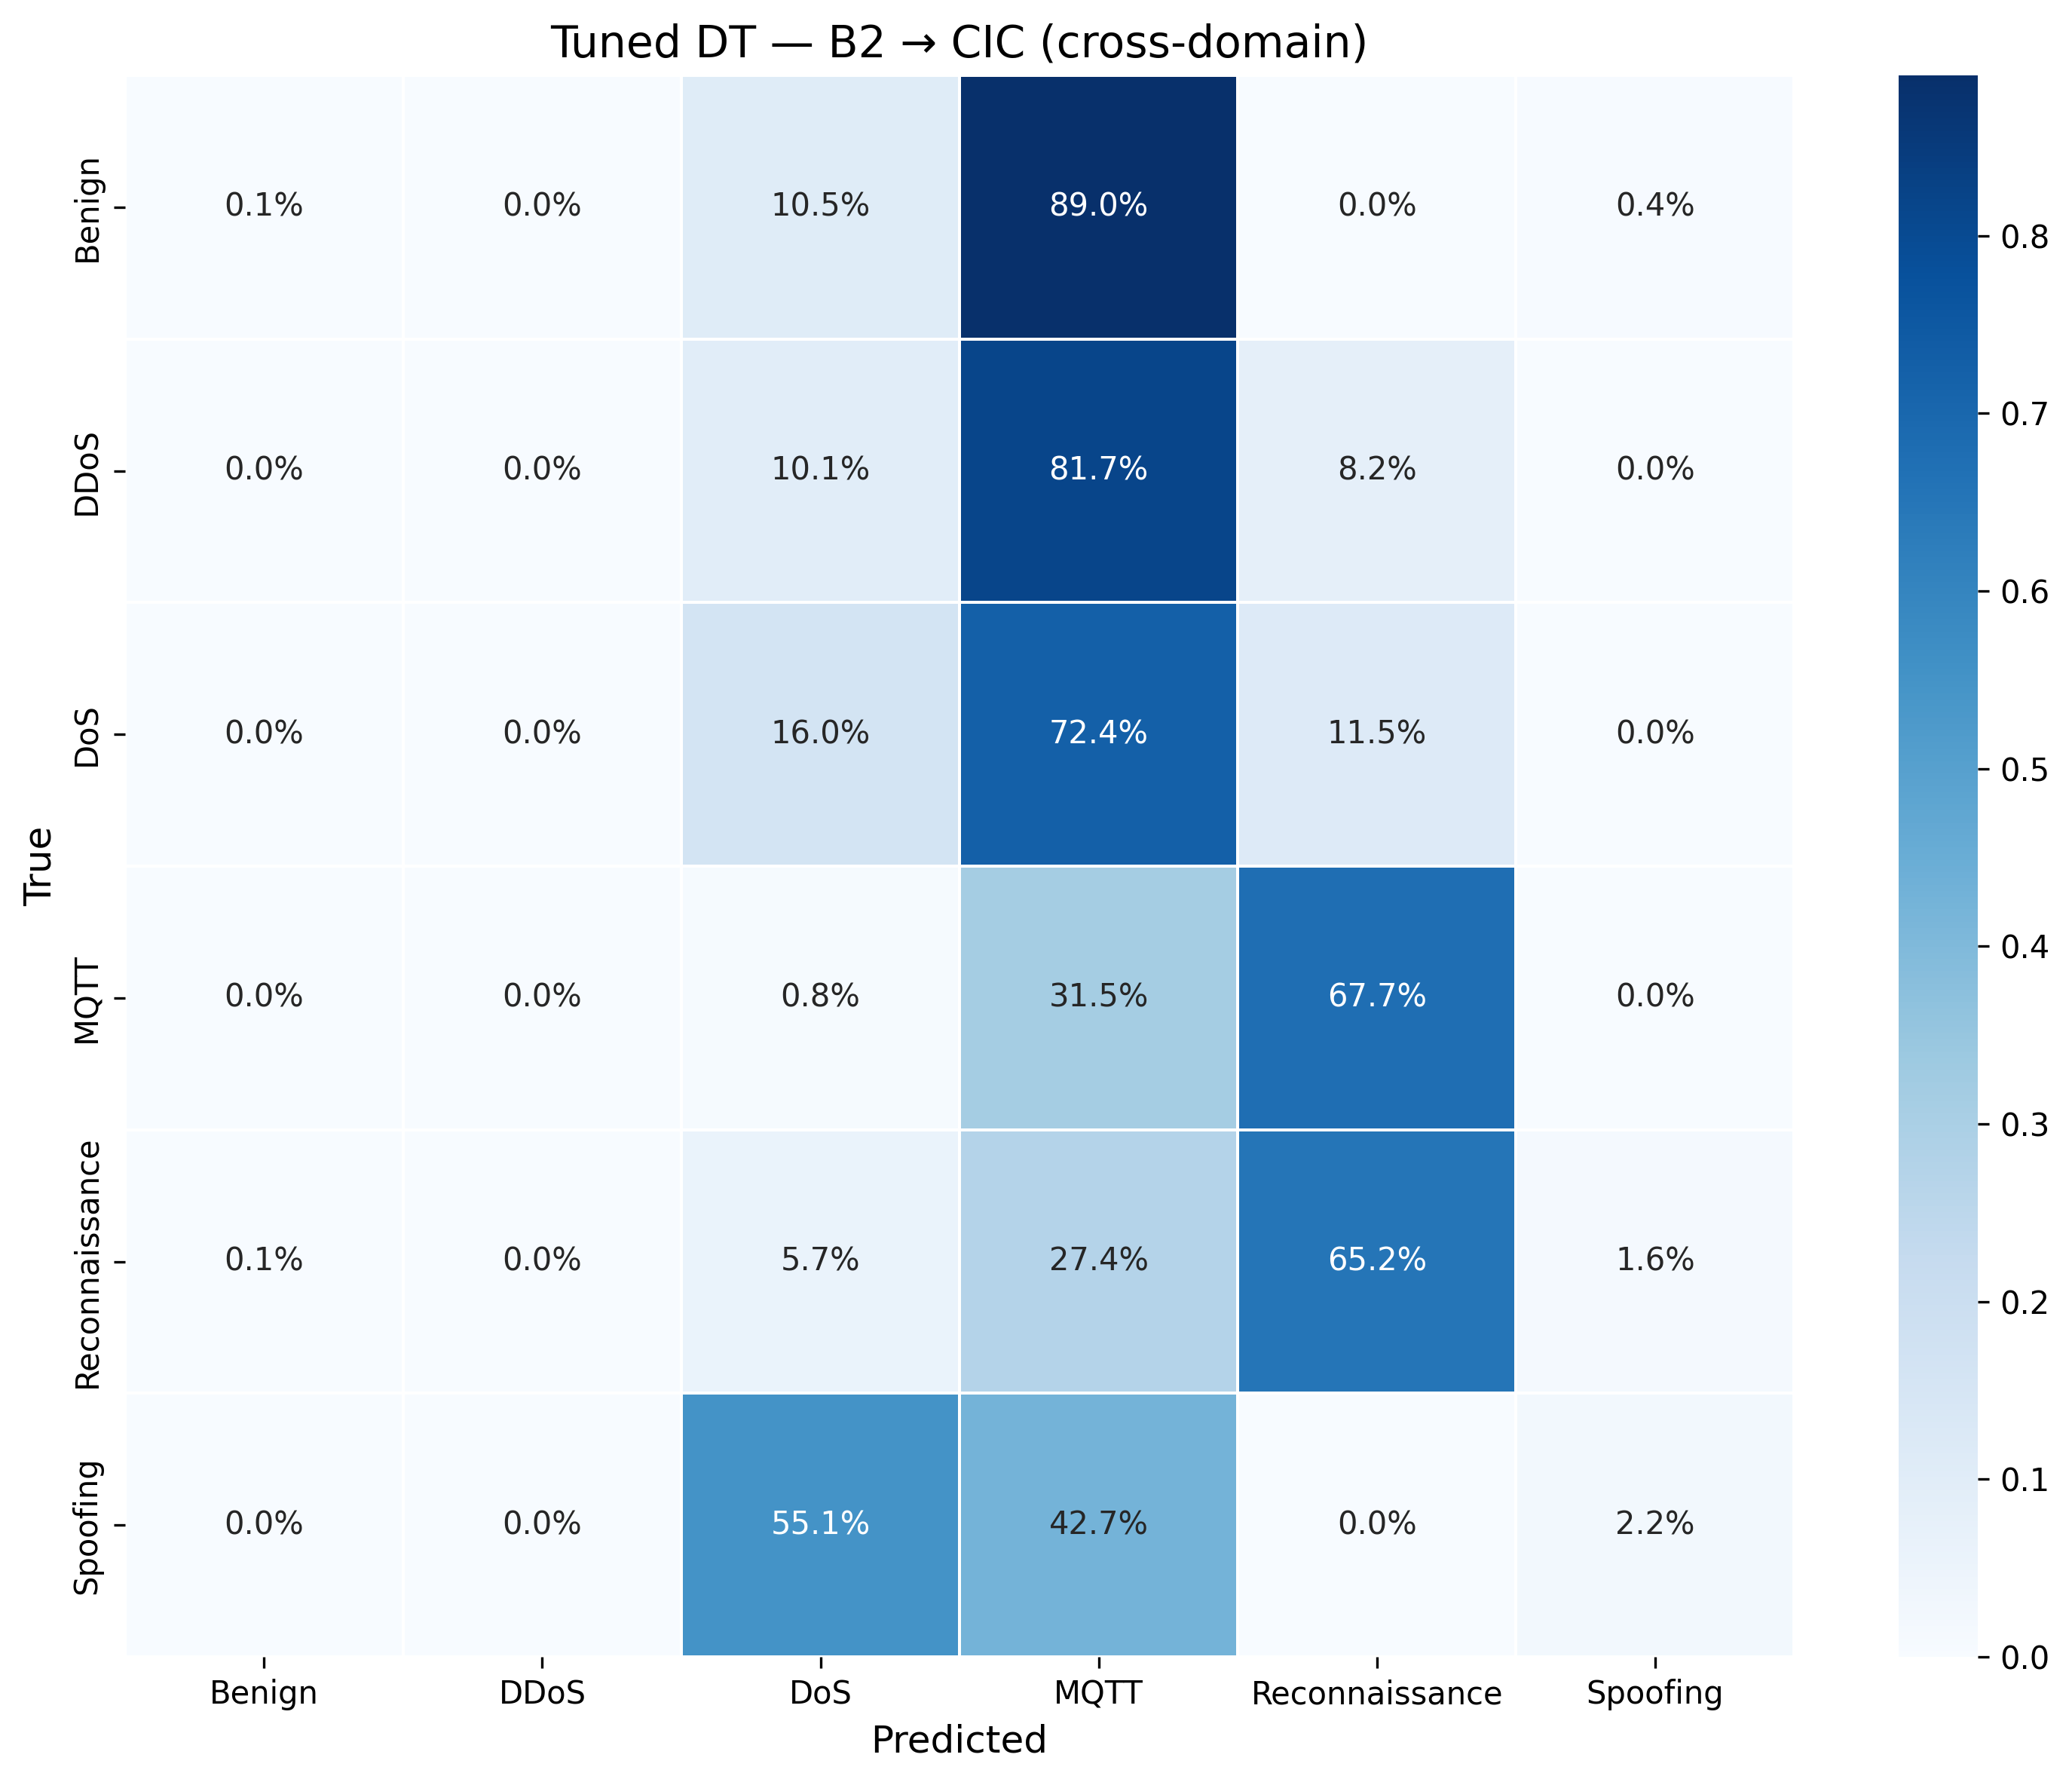
\includegraphics[width=\textwidth]{ch5_dt_cm_b2_xd_cic.png}
  \caption{B2 (IoMT-only) $\to$ CIC test}
\end{subfigure}
\caption{Cross-domain confusion matrices. Single-source models struggle with attack categories absent from their training data.}
\label{fig:dt-cm-xd}
\end{figure}

\subsubsection{Feature Importance}

Figure~\ref{fig:dt-feature-importance} presents the top-20 most important features for the tuned unified DT, measured by Gini importance. Figure~\ref{fig:dt-fi-comparison} compares feature importance rankings across all three regimes, revealing which features are universally discriminative versus source-specific.

\begin{figure}[H]
\centering
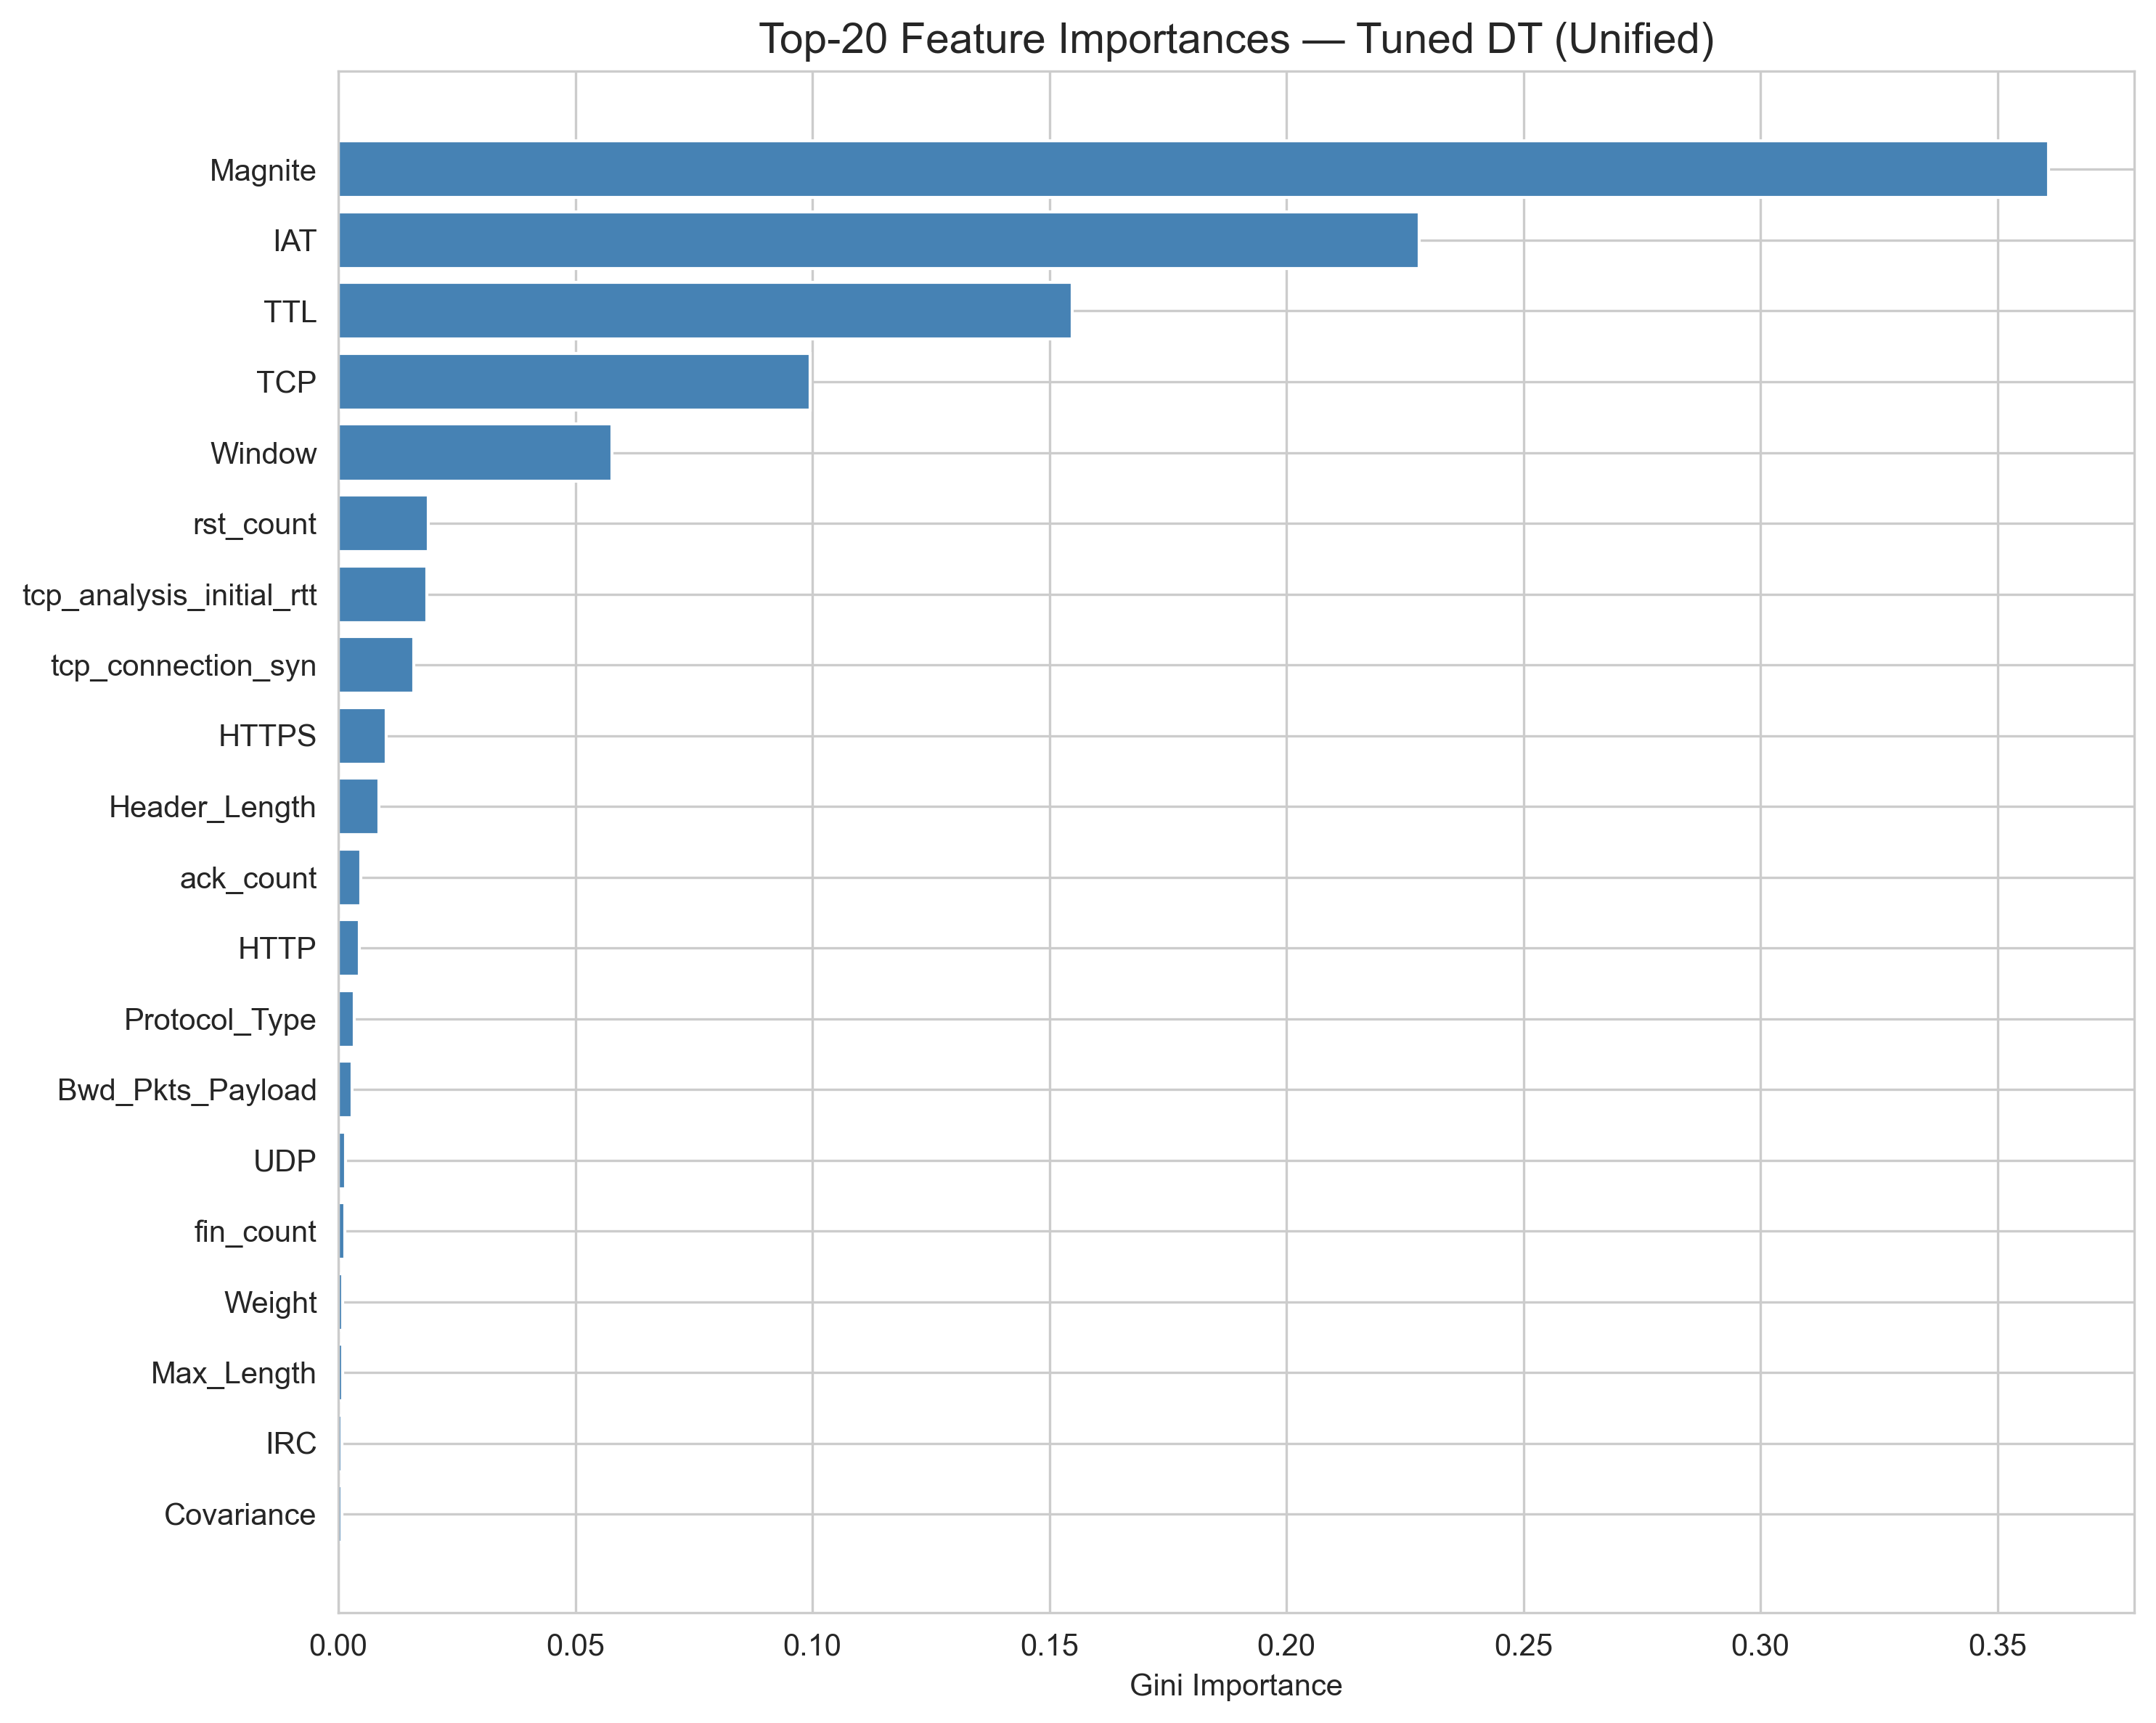
\includegraphics[width=0.85\textwidth]{ch5_dt_feature_importance_unified.png}
\caption{Top-20 feature importances for the tuned Decision Tree (Unified regime).}
\label{fig:dt-feature-importance}
\end{figure}

\begin{figure}[H]
\centering
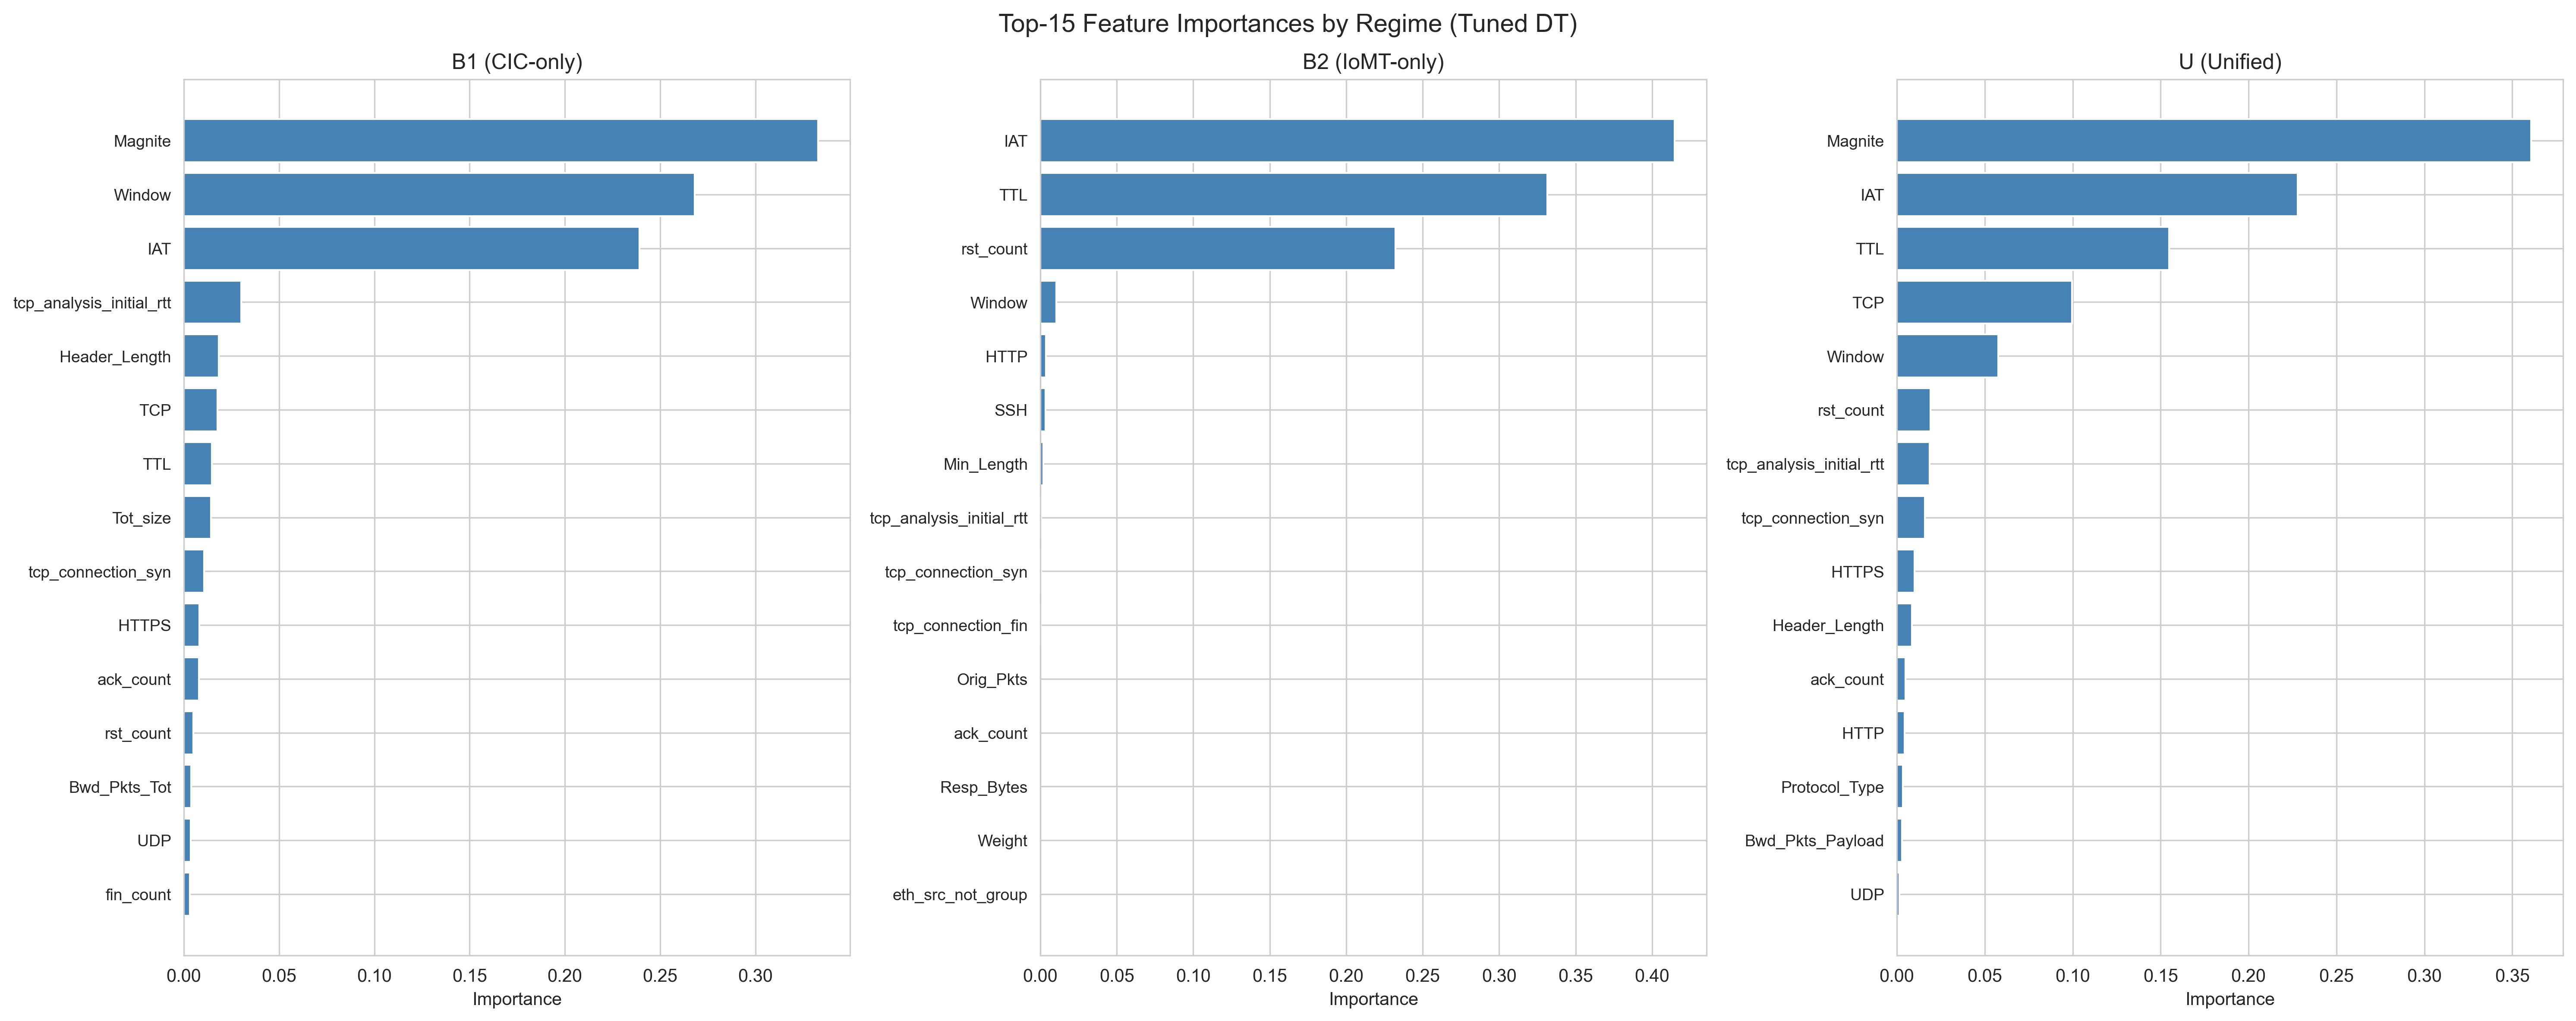
\includegraphics[width=\textwidth]{ch5_dt_feature_importance_comparison.png}
\caption{Feature importance comparison across the three training regimes (tuned DT, top-15).}
\label{fig:dt-fi-comparison}
\end{figure}

\subsubsection{Per-Class Analysis}

Figure~\ref{fig:dt-per-class-f1} breaks down F1-score by class for each tuned regime on the full test set. Table~\ref{tab:dt-perclass-unified} presents the detailed per-class metrics for the tuned unified model.

\begin{figure}[H]
\centering
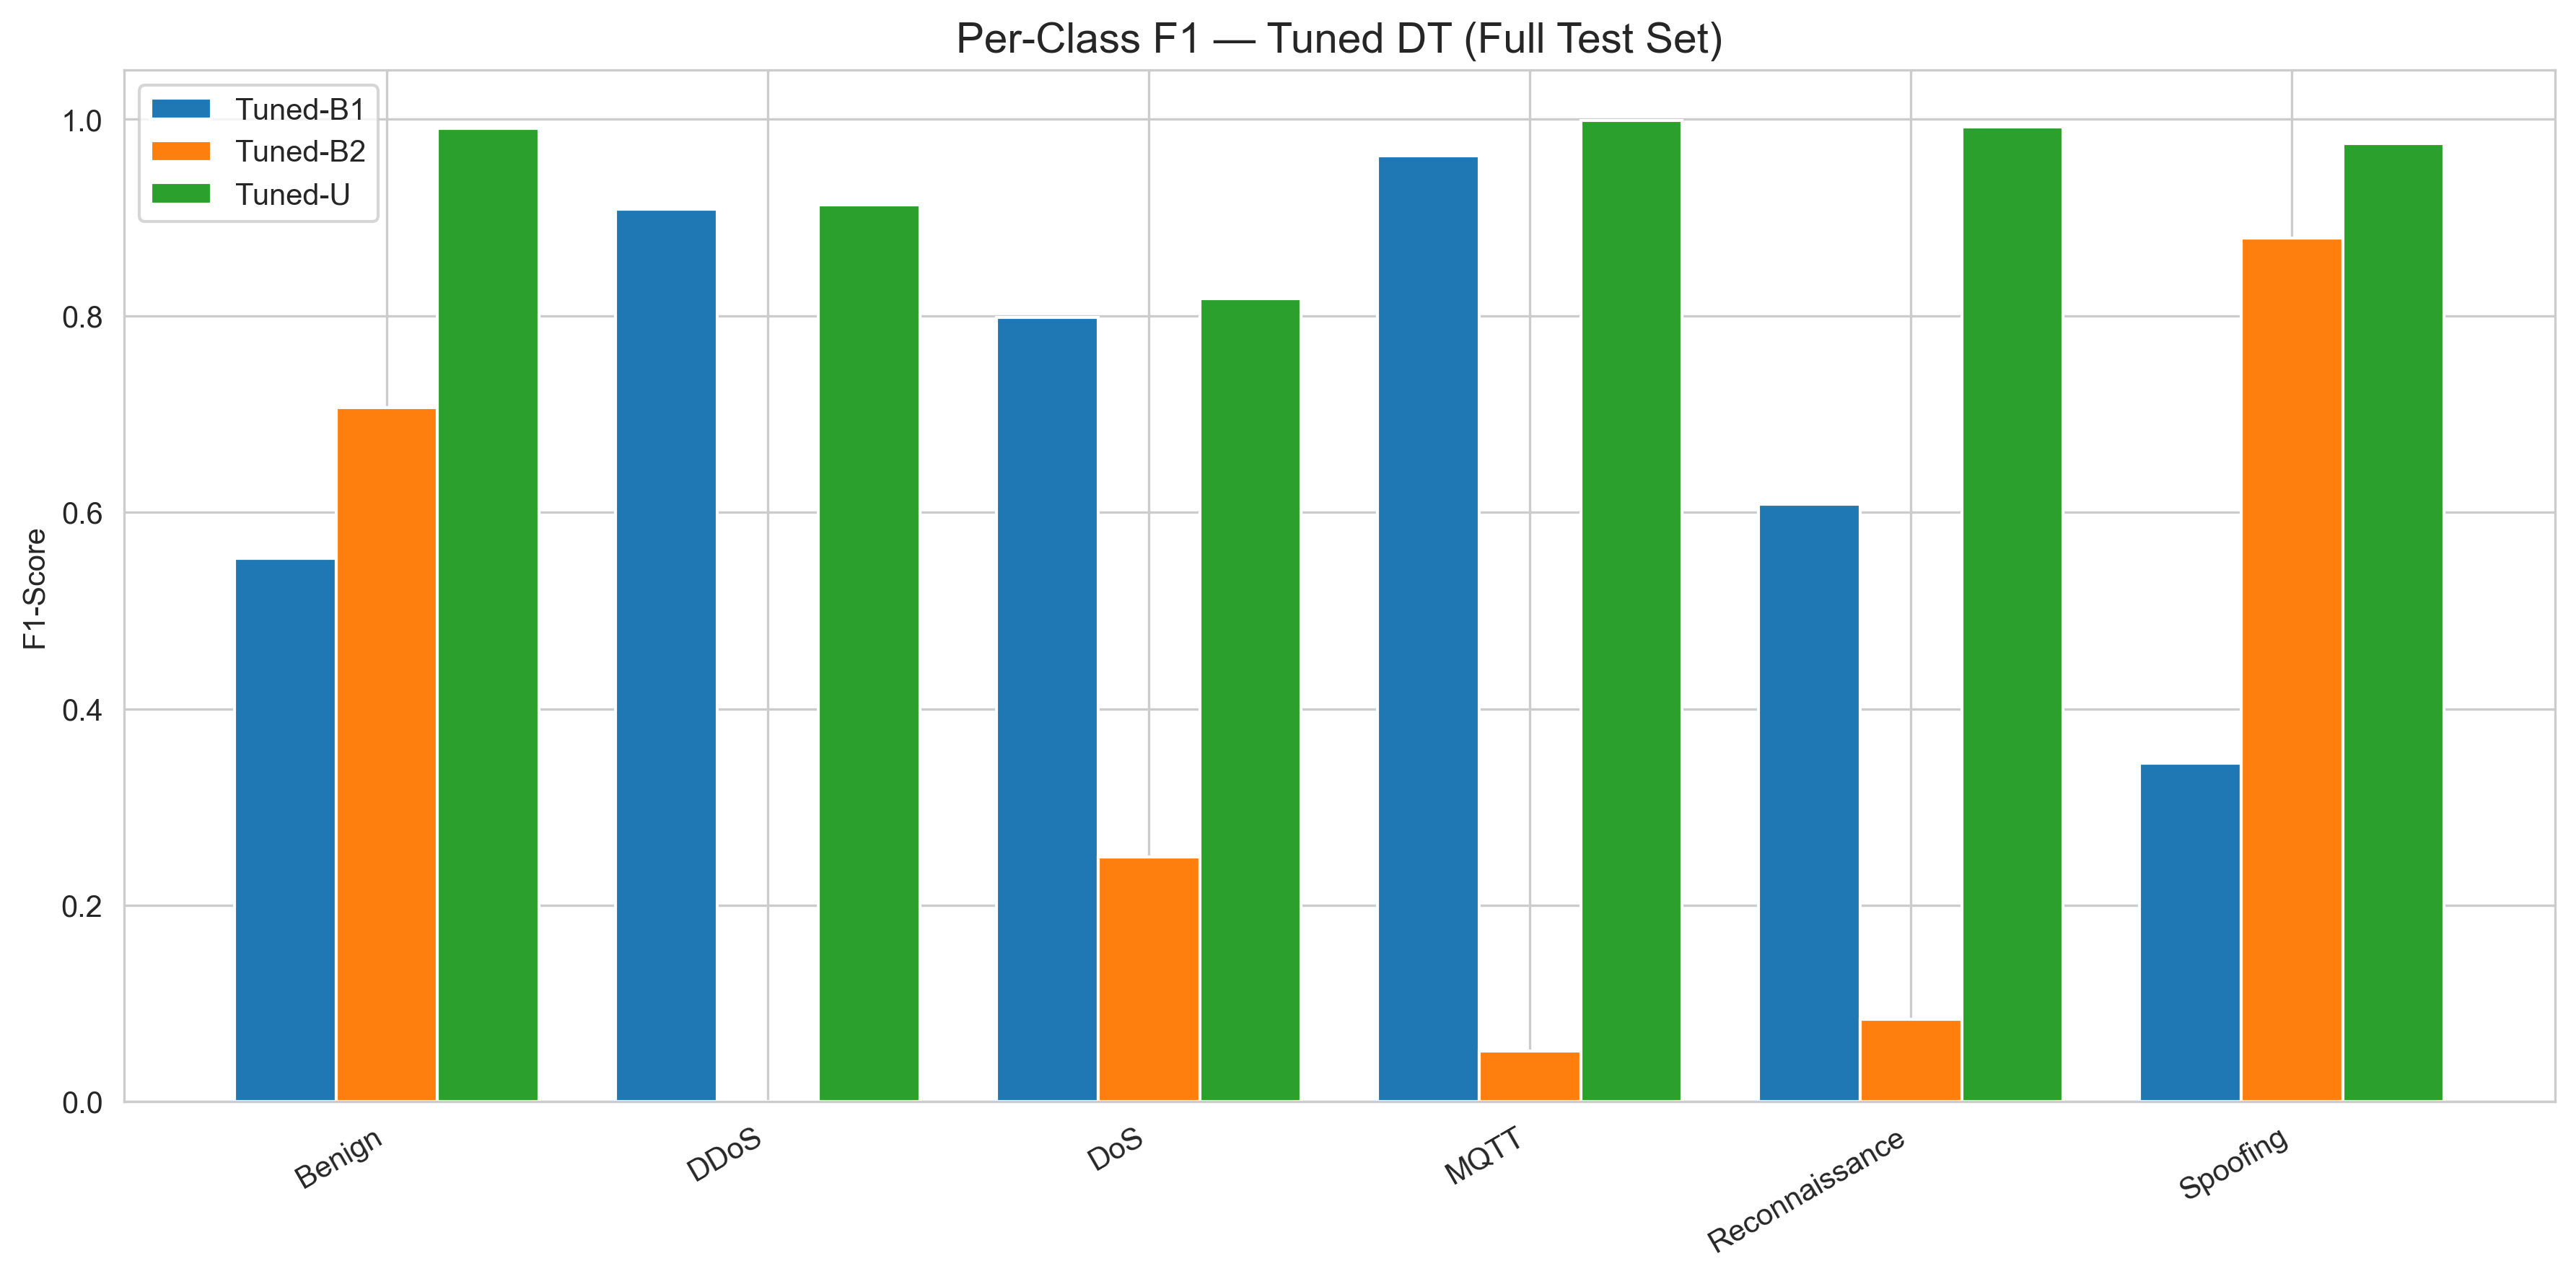
\includegraphics[width=0.85\textwidth]{ch5_dt_per_class_f1.png}
\caption{Per-class F1-score comparison across regimes (tuned DT, full test set).}
\label{fig:dt-per-class-f1}
\end{figure}

\begin{table}[H]
\centering
\caption{Per-class classification report for the tuned unified Decision Tree on the full test set (1,201,731 samples).}
\label{tab:dt-perclass-unified}
\small
\begin{tabular}{@{}l r r r r@{}}
\toprule
\textbf{Class} & \textbf{Precision} & \textbf{Recall} & \textbf{F1-Score} & \textbf{Support} \\
\midrule
Benign          & 0.99 & 1.00 & 0.99 &     8,018 \\
DDoS            & 0.97 & 0.86 & 0.91 &   805,244 \\
DoS             & 0.73 & 0.93 & 0.82 &   322,273 \\
MQTT            & 1.00 & 1.00 & 1.00 &    57,891 \\
Reconnaissance  & 0.99 & 0.99 & 0.99 &     6,904 \\
Spoofing        & 0.97 & 0.98 & 0.98 &     1,401 \\
\midrule
Accuracy        &      &      & 0.89 & 1,201,731 \\
Macro avg       & 0.94 & 0.96 & 0.95 & 1,201,731 \\
Weighted avg    & 0.91 & 0.89 & 0.89 & 1,201,731 \\
\bottomrule
\end{tabular}
\end{table}

The per-class results reveal a three-tier performance structure:

\paragraph{Tier 1 --- Near-perfect detection (F1 $\geq$ 0.98).}
MQTT (F1\,=\,1.00), Benign (0.99), Reconnaissance (0.99), and Spoofing (0.98) are classified with near-zero error. The MQTT class benefits from its distinct protocol-level features (MQTT-specific packet patterns). Benign and Reconnaissance traffic are also well-separated in the 58-feature space. Notably, Spoofing achieves F1\,=\,0.98 despite representing only 0.12\% of the test data (1,401 samples), confirming that the balanced class weights successfully compensated for extreme rarity. This success is also attributable to the distinctive network fingerprint of ARP Spoofing, which produces characteristic patterns in features such as \texttt{eth\_src\_not\_group} and \texttt{TTL}.

\paragraph{Tier 2 --- The DDoS/DoS confusion boundary.}
DDoS (F1\,=\,0.91) and DoS (F1\,=\,0.82) are the only classes with substantial error. Detailed inspection of the confusion matrix (Figure~\ref{fig:dt-confusion-unified}) reveals that 109,220 DDoS samples (13.6\%) are misclassified as DoS, and 24,020 DoS samples (7.5\%) are misclassified as DDoS. These 133,240 cross-confused samples account for \textbf{99.8\% of all classification errors} across the entire test set. This asymmetry manifests as:
\begin{itemize}[nosep]
  \item \textbf{DDoS}: High precision (0.97) but reduced recall (0.86) --- the model rarely labels a non-DDoS sample as DDoS, but misses 14\% of true DDoS traffic by labeling it DoS.
  \item \textbf{DoS}: High recall (0.93) but reduced precision (0.73) --- the model catches most DoS attacks, but also absorbs many DDoS samples as false positives.
\end{itemize}

This confusion is \textit{expected} and reflects a fundamental characteristic of the feature space: TCP/IP-based DDoS and DoS attacks (SYN floods, ICMP floods, UDP floods, TCP floods) share nearly identical per-window network statistics. The distinguishing factor---the number of attacking sources---is not directly captured by the 58 MIOTTA features, which aggregate flows within a time window without retaining source-level diversity information.

\paragraph{Accuracy vs.\ macro-F1 discrepancy.}
The overall accuracy (0.89) appears lower than the macro-F1 (0.95) because accuracy is dominated by the majority class: DDoS constitutes 67\% of the test data, and its recall of 0.86 drags down the global accuracy. In contrast, macro-F1 gives equal weight to each class, thereby reflecting the excellent performance on all four minority classes. For IDS evaluation on imbalanced datasets, macro-F1 is the more informative metric, as discussed in Section~\ref{subsec:experimental-setup}.

\subsubsection{Summary}

The Decision Tree experiments establish clear empirical evidence regarding the benefit of multi-source integration:

\begin{itemize}[nosep]
  \item \textbf{Single-source models fail cross-domain.} B1 achieves macro-F1 = 0.9226 in-domain but only 0.2474 on IoMT data. B2 achieves 0.8332 in-domain but collapses to 0.0523 on CIC data---unable to recognize DDoS traffic it has never seen.
  \item \textbf{Unified training resolves the gap.} The tuned unified DT achieves macro-F1 = 0.9480 on the full test set, outperforming both baselines on every cross-domain slice. This is a +25.2 percentage-point absolute improvement (or +36.2\% relative) over the best single-source model (B1) on the full test.
  \item \textbf{Tuning yields modest gains.} Hyperparameter tuning improved all three regimes: B1 (+2.8\%), B2 (--0.3\%), U (+1.1\%) on their respective full-test macro-F1. The selected hyperparameters favor shallower trees (\texttt{max\_depth}=15) with entropy criterion, reducing overfitting compared to the unlimited-depth baseline.
  \item \textbf{Class-level analysis.} Four of six categories (Benign, MQTT, Reconnaissance, Spoofing) achieve F1 $\geq$ 0.98, confirming that balanced class weights effectively address extreme imbalance. The only significant weakness is the DDoS/DoS confusion boundary (133,240 cross-misclassified samples, 99.8\% of all errors), attributable to the inherent similarity of these attack families at the network-feature level. Ensemble methods (RF, XGBoost) are expected to improve this boundary through their capacity for more nuanced decision boundaries.
\end{itemize}

Detailed discussion of these results, in the context of the other classifiers and the research question, is deferred to Section~\ref{subsec:discussion}.

\subsection{Random Forest Classifier}
\label{subsec:random-forest}

The Random Forest (RF) extends the Decision Tree with bagging and feature randomization, averaging predictions over an ensemble of decorrelated trees. The same three-regime protocol applies: baseline (100 trees, balanced class weights) followed by tuned models from \texttt{RandomizedSearchCV} (50 iterations, 3-fold CV, macro-F1 scoring), with the subsample-then-full-refit procedure described above for computational feasibility.

\subsubsection{Baseline Results}

Table~\ref{tab:rf-baseline} reports baseline RF performance. Patterns mirror the Decision Tree: single-source models achieve strong in-domain scores but degrade sharply on the opposite source's test slice.

\begin{table}[H]
\centering
\caption{Baseline Random Forest (100 trees, balanced class weights) evaluation matrix.}
\label{tab:rf-baseline}
\small
\begin{tabular}{@{}l l c c c@{}}
\toprule
\textbf{Regime} & \textbf{Test slice} & \textbf{Macro-F1} & \textbf{Weighted-F1} & \textbf{Accuracy} \\
\midrule
B1 (CIC-only) & CIC (in-domain)  & 0.9175 & 0.8744 & 0.8743 \\
B1 (CIC-only) & IoMT (cross)     & 0.1982 & 0.3601 & 0.3903 \\
B1 (CIC-only) & Full             & 0.6677 & 0.8615 & 0.8631 \\
\midrule
B2 (IoMT-only) & IoMT (in-domain) & 0.8333 & 1.0000 & 1.0000 \\
B2 (IoMT-only) & CIC (cross)      & 0.1570 & 0.1226 & 0.2420 \\
B2 (IoMT-only) & Full             & 0.2945 & 0.1350 & 0.2594 \\
\midrule
U (Unified)    & CIC              & 0.9178 & 0.8744 & 0.8743 \\
U (Unified)    & IoMT             & 0.8330 & 0.9996 & 0.9996 \\
U (Unified)    & Full             & \textbf{0.9404} & 0.8772 & 0.8771 \\
\bottomrule
\end{tabular}
\end{table}

\subsubsection{Tuned Results}

Table~\ref{tab:rf-tuned} reports tuned RF results. Table~\ref{tab:rf-best-params} lists the selected hyperparameters and cross-validated macro-F1 on the search subsample (or full training set for B2).

\begin{table}[H]
\centering
\caption{Tuned Random Forest evaluation matrix.}
\label{tab:rf-tuned}
\small
\begin{tabular}{@{}l l c c c@{}}
\toprule
\textbf{Regime} & \textbf{Test slice} & \textbf{Macro-F1} & \textbf{Weighted-F1} & \textbf{Accuracy} \\
\midrule
Tuned B1 & CIC (in-domain)  & 0.9149 & 0.8903 & 0.8866 \\
Tuned B1 & IoMT (cross)     & 0.3423 & 0.5013 & 0.5089 \\
Tuned B1 & Full             & 0.7395 & 0.8811 & 0.8779 \\
\midrule
Tuned B2 & IoMT (in-domain) & 0.8333 & 1.0000 & 1.0000 \\
Tuned B2 & CIC (cross)      & 0.0586 & 0.0537 & 0.0707 \\
Tuned B2 & Full             & 0.2029 & 0.0680 & 0.0921 \\
\midrule
Tuned U  & CIC              & 0.9285 & 0.8895 & 0.8858 \\
Tuned U  & IoMT             & 0.8329 & 0.9995 & 0.9995 \\
Tuned U  & Full             & \textbf{0.9487} & 0.8919 & 0.8884 \\
\bottomrule
\end{tabular}
\end{table}

\paragraph{Note on Macro-F1 (IoMT slice, Tuned U).}
The IoMT-only test slice contains no DDoS samples; accordingly, the global six-class Macro-F1 reported for the Random Forest on that slice (0.8329) averages over a zero-score DDoS column, following the same convention as the Decision Tree table. Weighted-F1 and accuracy remain near-perfect on the same slice because those metrics are support-weighted and are not penalized by an absent class.

\begin{table}[H]
\centering
\caption{Best hyperparameters per regime (Random Forest, 50-iteration RandomizedSearchCV). CV F1m is the best cross-validated macro-F1 on the training fold used during search.}
\label{tab:rf-best-params}
\small
\begin{tabular}{@{}l c c c c c c c@{}}
\toprule
\textbf{Regime} & \textbf{trees} & \textbf{depth} & \textbf{mss} & \textbf{msl} & \textbf{max\_feat.} & \textbf{max\_samp.} & \textbf{CV F1m} \\
\midrule
B1 (CIC-only)  & 200 & 15 & 5 & 1 & 0.5 & 0.8 & 0.9024 \\
B2 (IoMT-only) & 300 & 15 & 5 & 1 & 0.3 & 0.8 & 0.9999 \\
U (Unified)    & 200 & 15 & 5 & 1 & 0.5 & 0.8 & 0.9390 \\
\bottomrule
\end{tabular}
\end{table}

\noindent\textit{Class weight:} B1 and U use \texttt{balanced}; B2 uses \texttt{balanced\_subsample}. All three regimes selected \texttt{max\_depth}=15 and \texttt{max\_samples}=0.8, indicating a preference for moderately deep trees with row subsampling per tree---a configuration that limits variance and memory footprint relative to unrestricted depth and full bootstrap samples.

\subsubsection{Cross-Domain Analysis}

Figure~\ref{fig:rf-confusion-unified} shows the normalized confusion matrix for the tuned unified RF on the full test set. Figure~\ref{fig:rf-cm-xd} shows the cross-domain matrices for B1$\to$IoMT and B2$\to$CIC.

\begin{figure}[H]
\centering
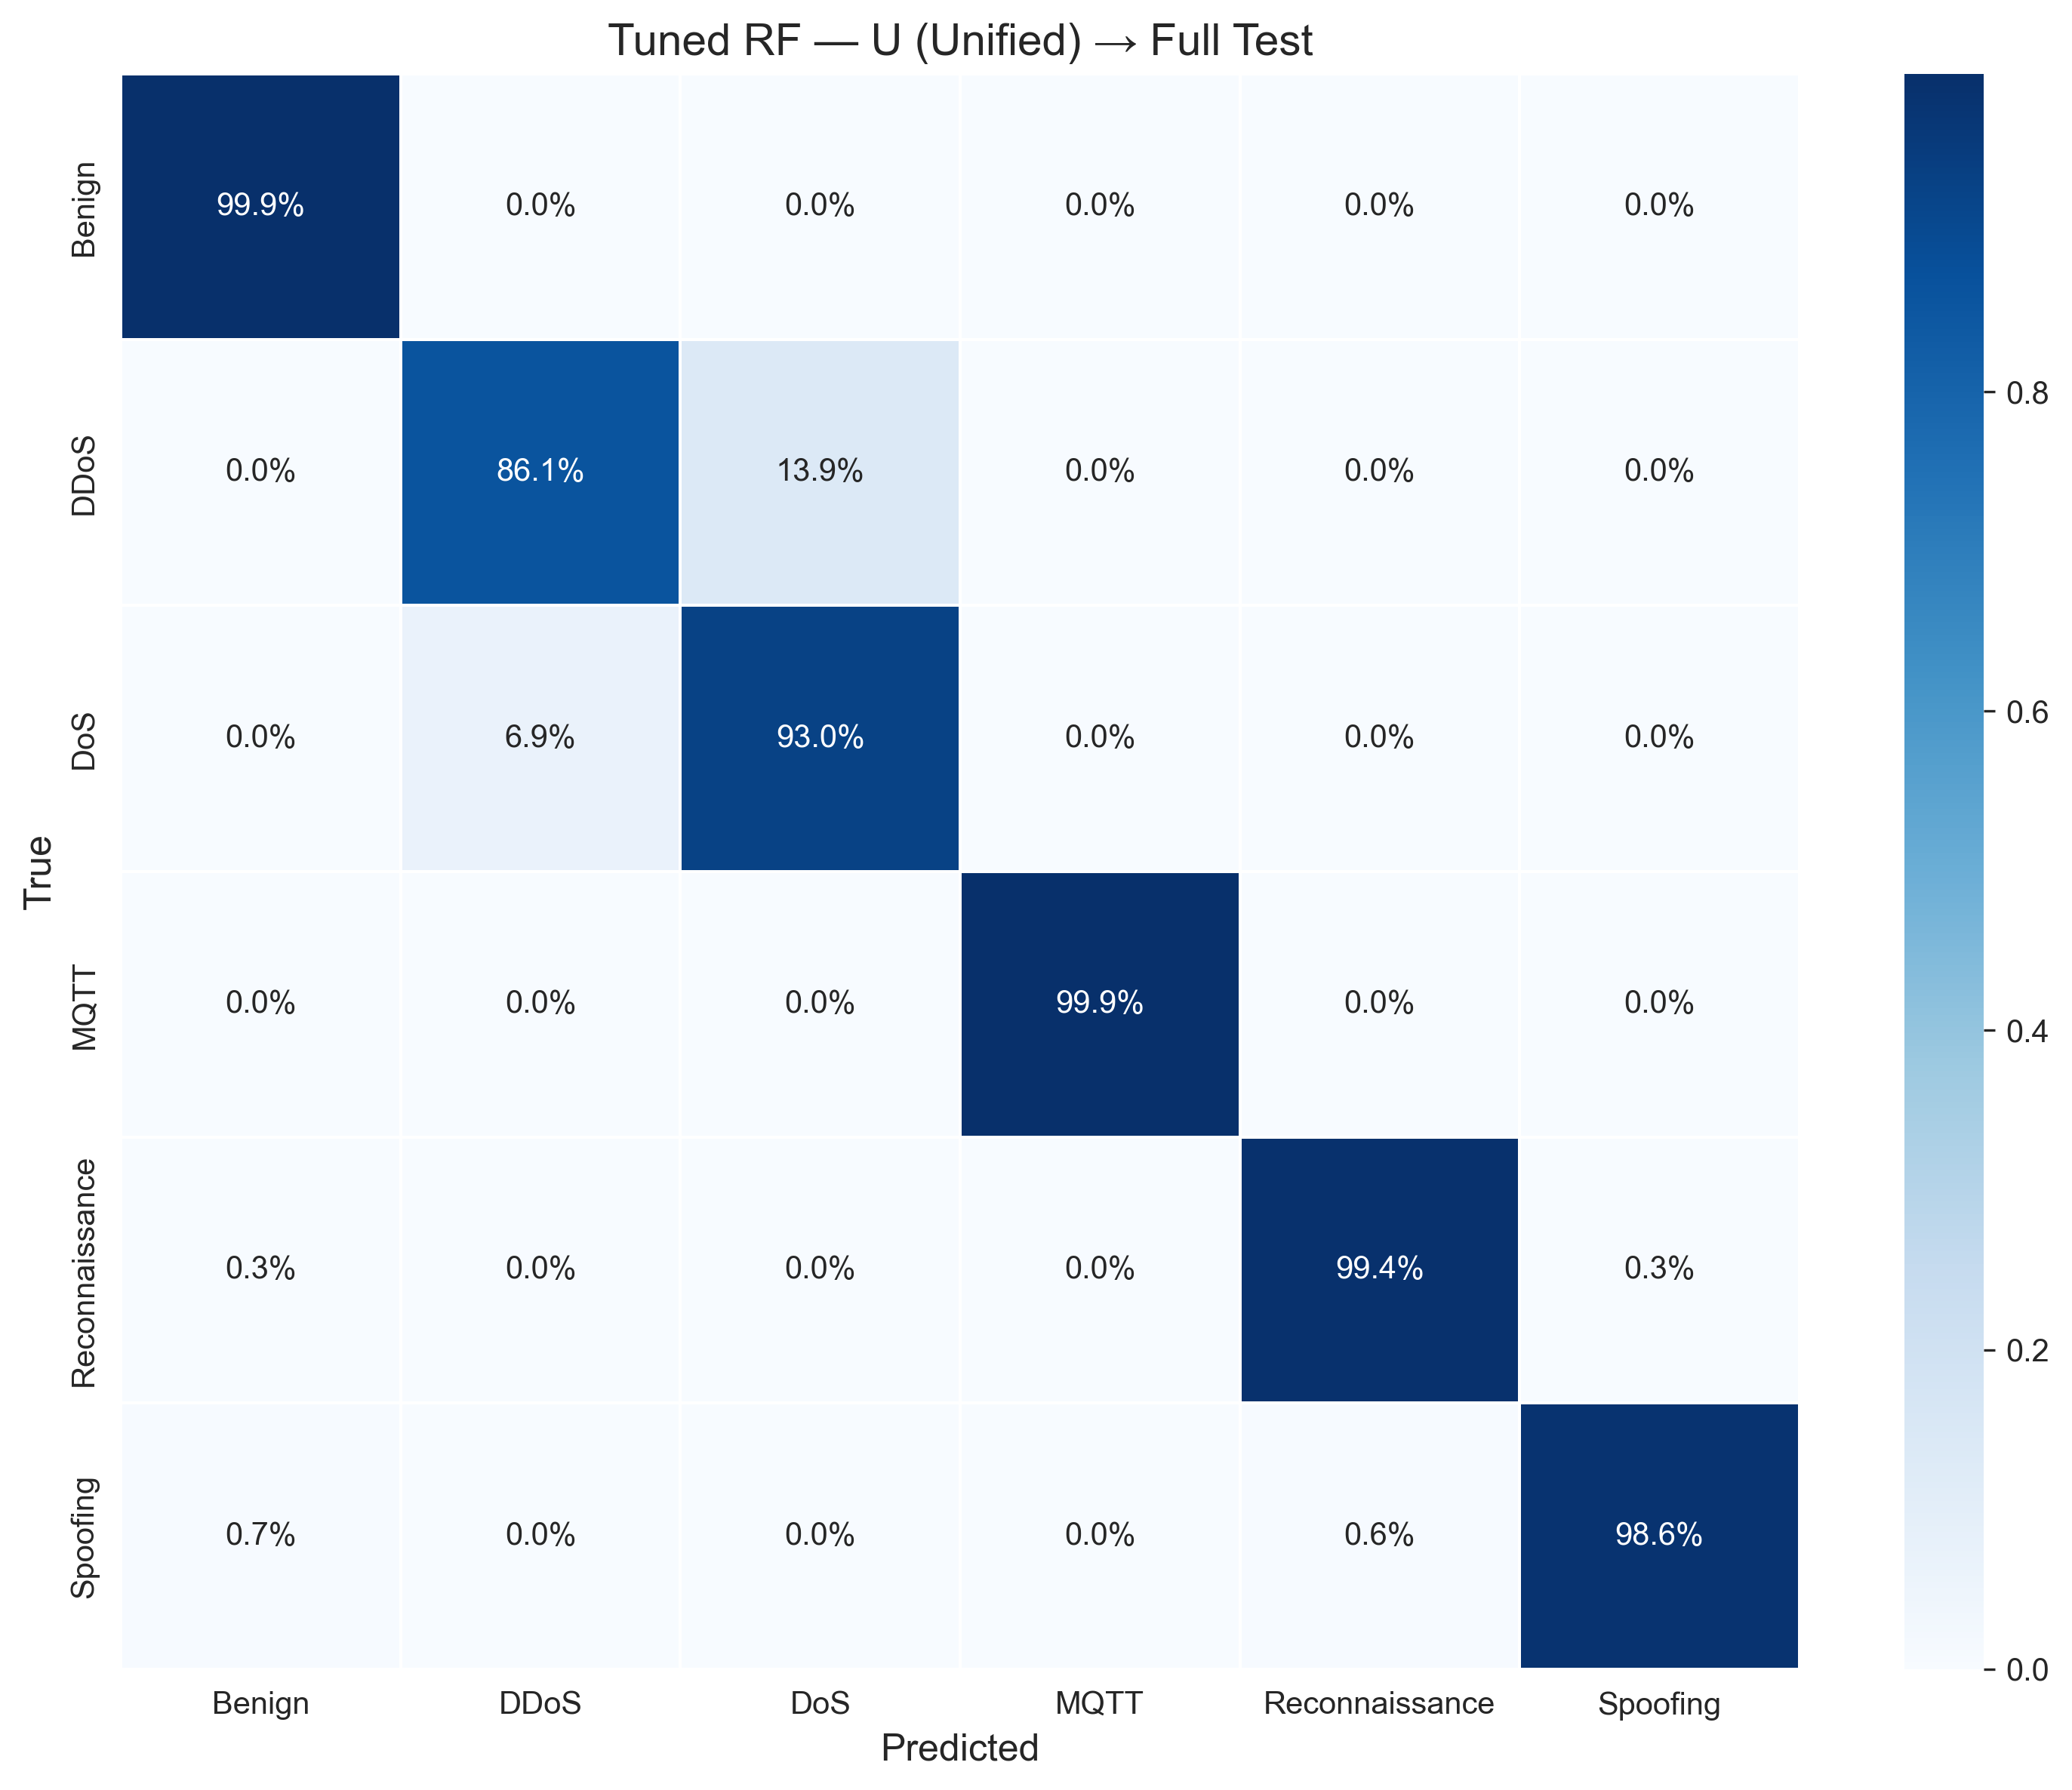
\includegraphics[width=0.75\textwidth]{ch5_rf_cm_u_full.png}
\caption{Normalized confusion matrix --- Tuned RF (Unified) on the full test set.}
\label{fig:rf-confusion-unified}
\end{figure}

\begin{figure}[H]
\centering
\begin{subfigure}[b]{0.48\textwidth}
  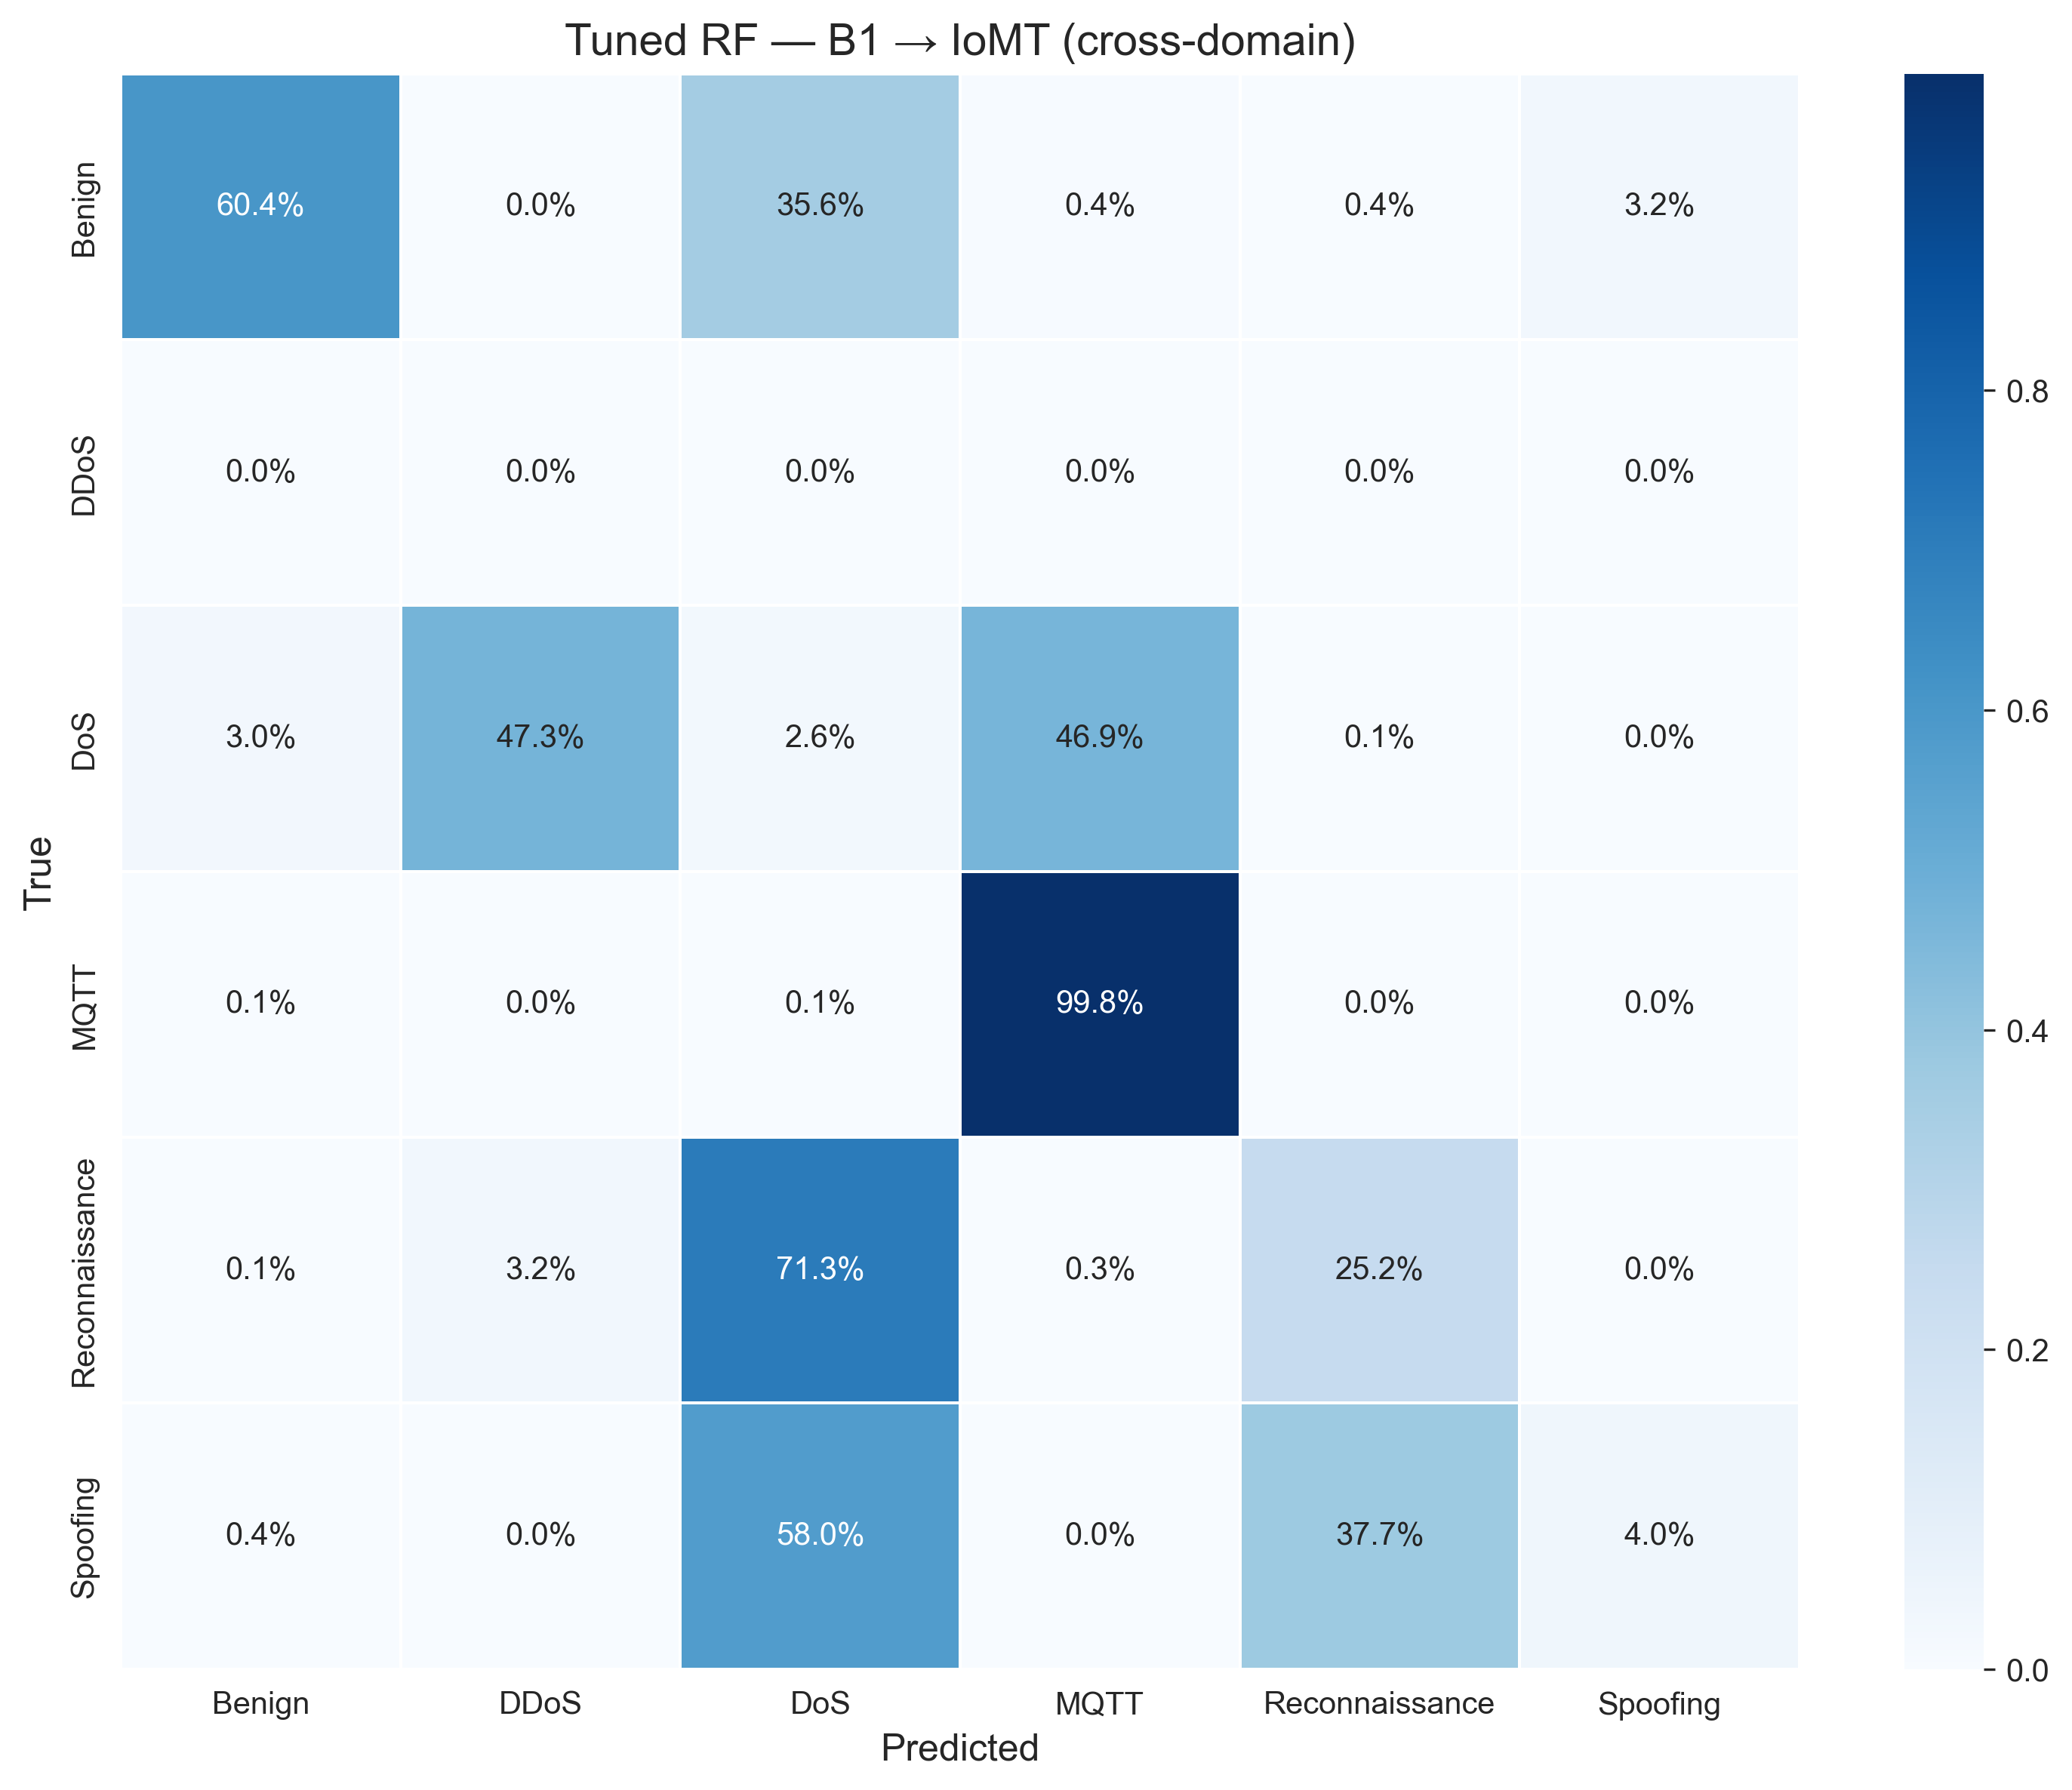
\includegraphics[width=\textwidth]{ch5_rf_cm_b1_xd_iomt.png}
  \caption{B1 (CIC-only) $\to$ IoMT test}
\end{subfigure}
\hfill
\begin{subfigure}[b]{0.48\textwidth}
  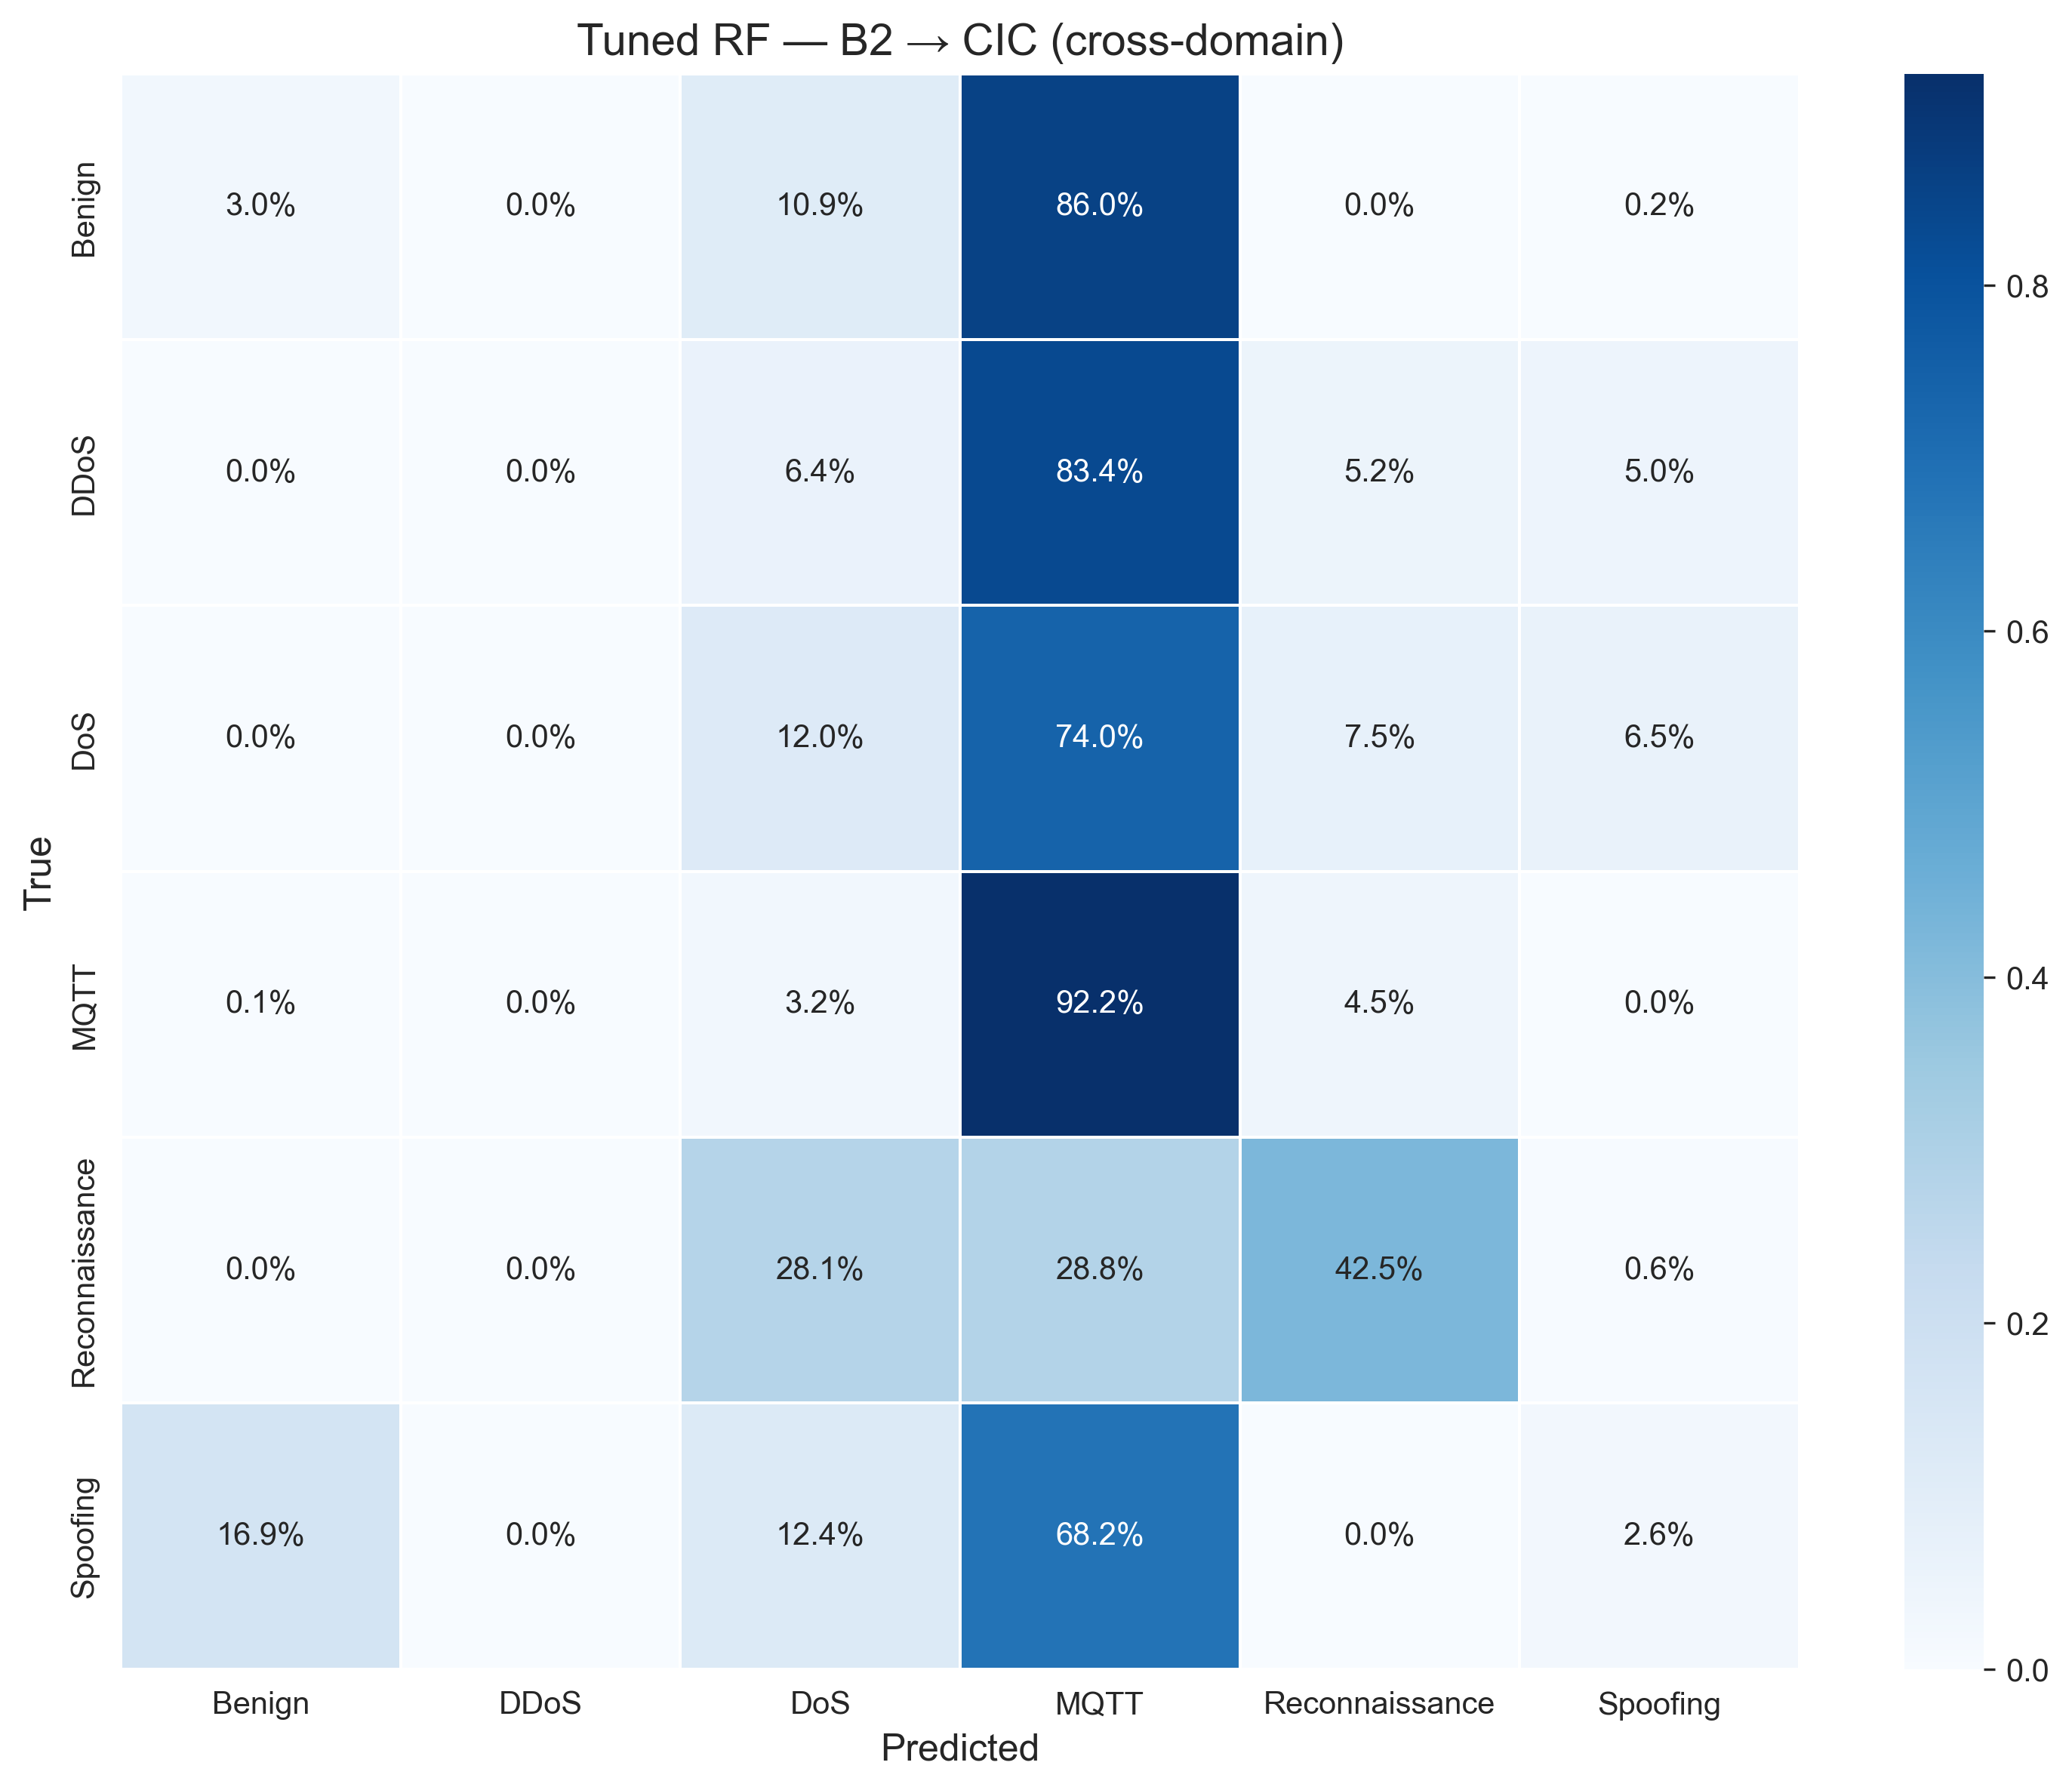
\includegraphics[width=\textwidth]{ch5_rf_cm_b2_xd_cic.png}
  \caption{B2 (IoMT-only) $\to$ CIC test}
\end{subfigure}
\caption{Cross-domain confusion matrices for tuned Random Forest models.}
\label{fig:rf-cm-xd}
\end{figure}

The unified RF confusion matrix (Figure~\ref{fig:rf-confusion-unified}) closely mirrors its Decision Tree counterpart: the dominant off-diagonal mass remains the bidirectional DDoS$\leftrightarrow$DoS confusion, while all other class pairs produce near-zero error. In the cross-domain scenario, the B1$\to$IoMT Macro-F1 (0.3423) is noticeably stronger than the equivalent DT score (0.2474), which suggests that bagging's variance reduction allows the ensemble to partially generalize CIC-trained feature patterns to the unseen IoMT distribution. The B2$\to$CIC result remains near-zero (0.0586) for the same structural reason as the Decision Tree: the IoMT-only model has never observed DDoS traffic, which constitutes the majority class of the CIC test slice, so the model cannot produce meaningful predictions on that slice regardless of its within-domain quality.

\subsubsection{Feature Importance}

Figure~\ref{fig:rf-feature-importance} and Figure~\ref{fig:rf-fi-comparison} show Gini-based importances for the tuned unified RF and a regime-wise comparison (top-15), respectively.

\begin{figure}[H]
\centering
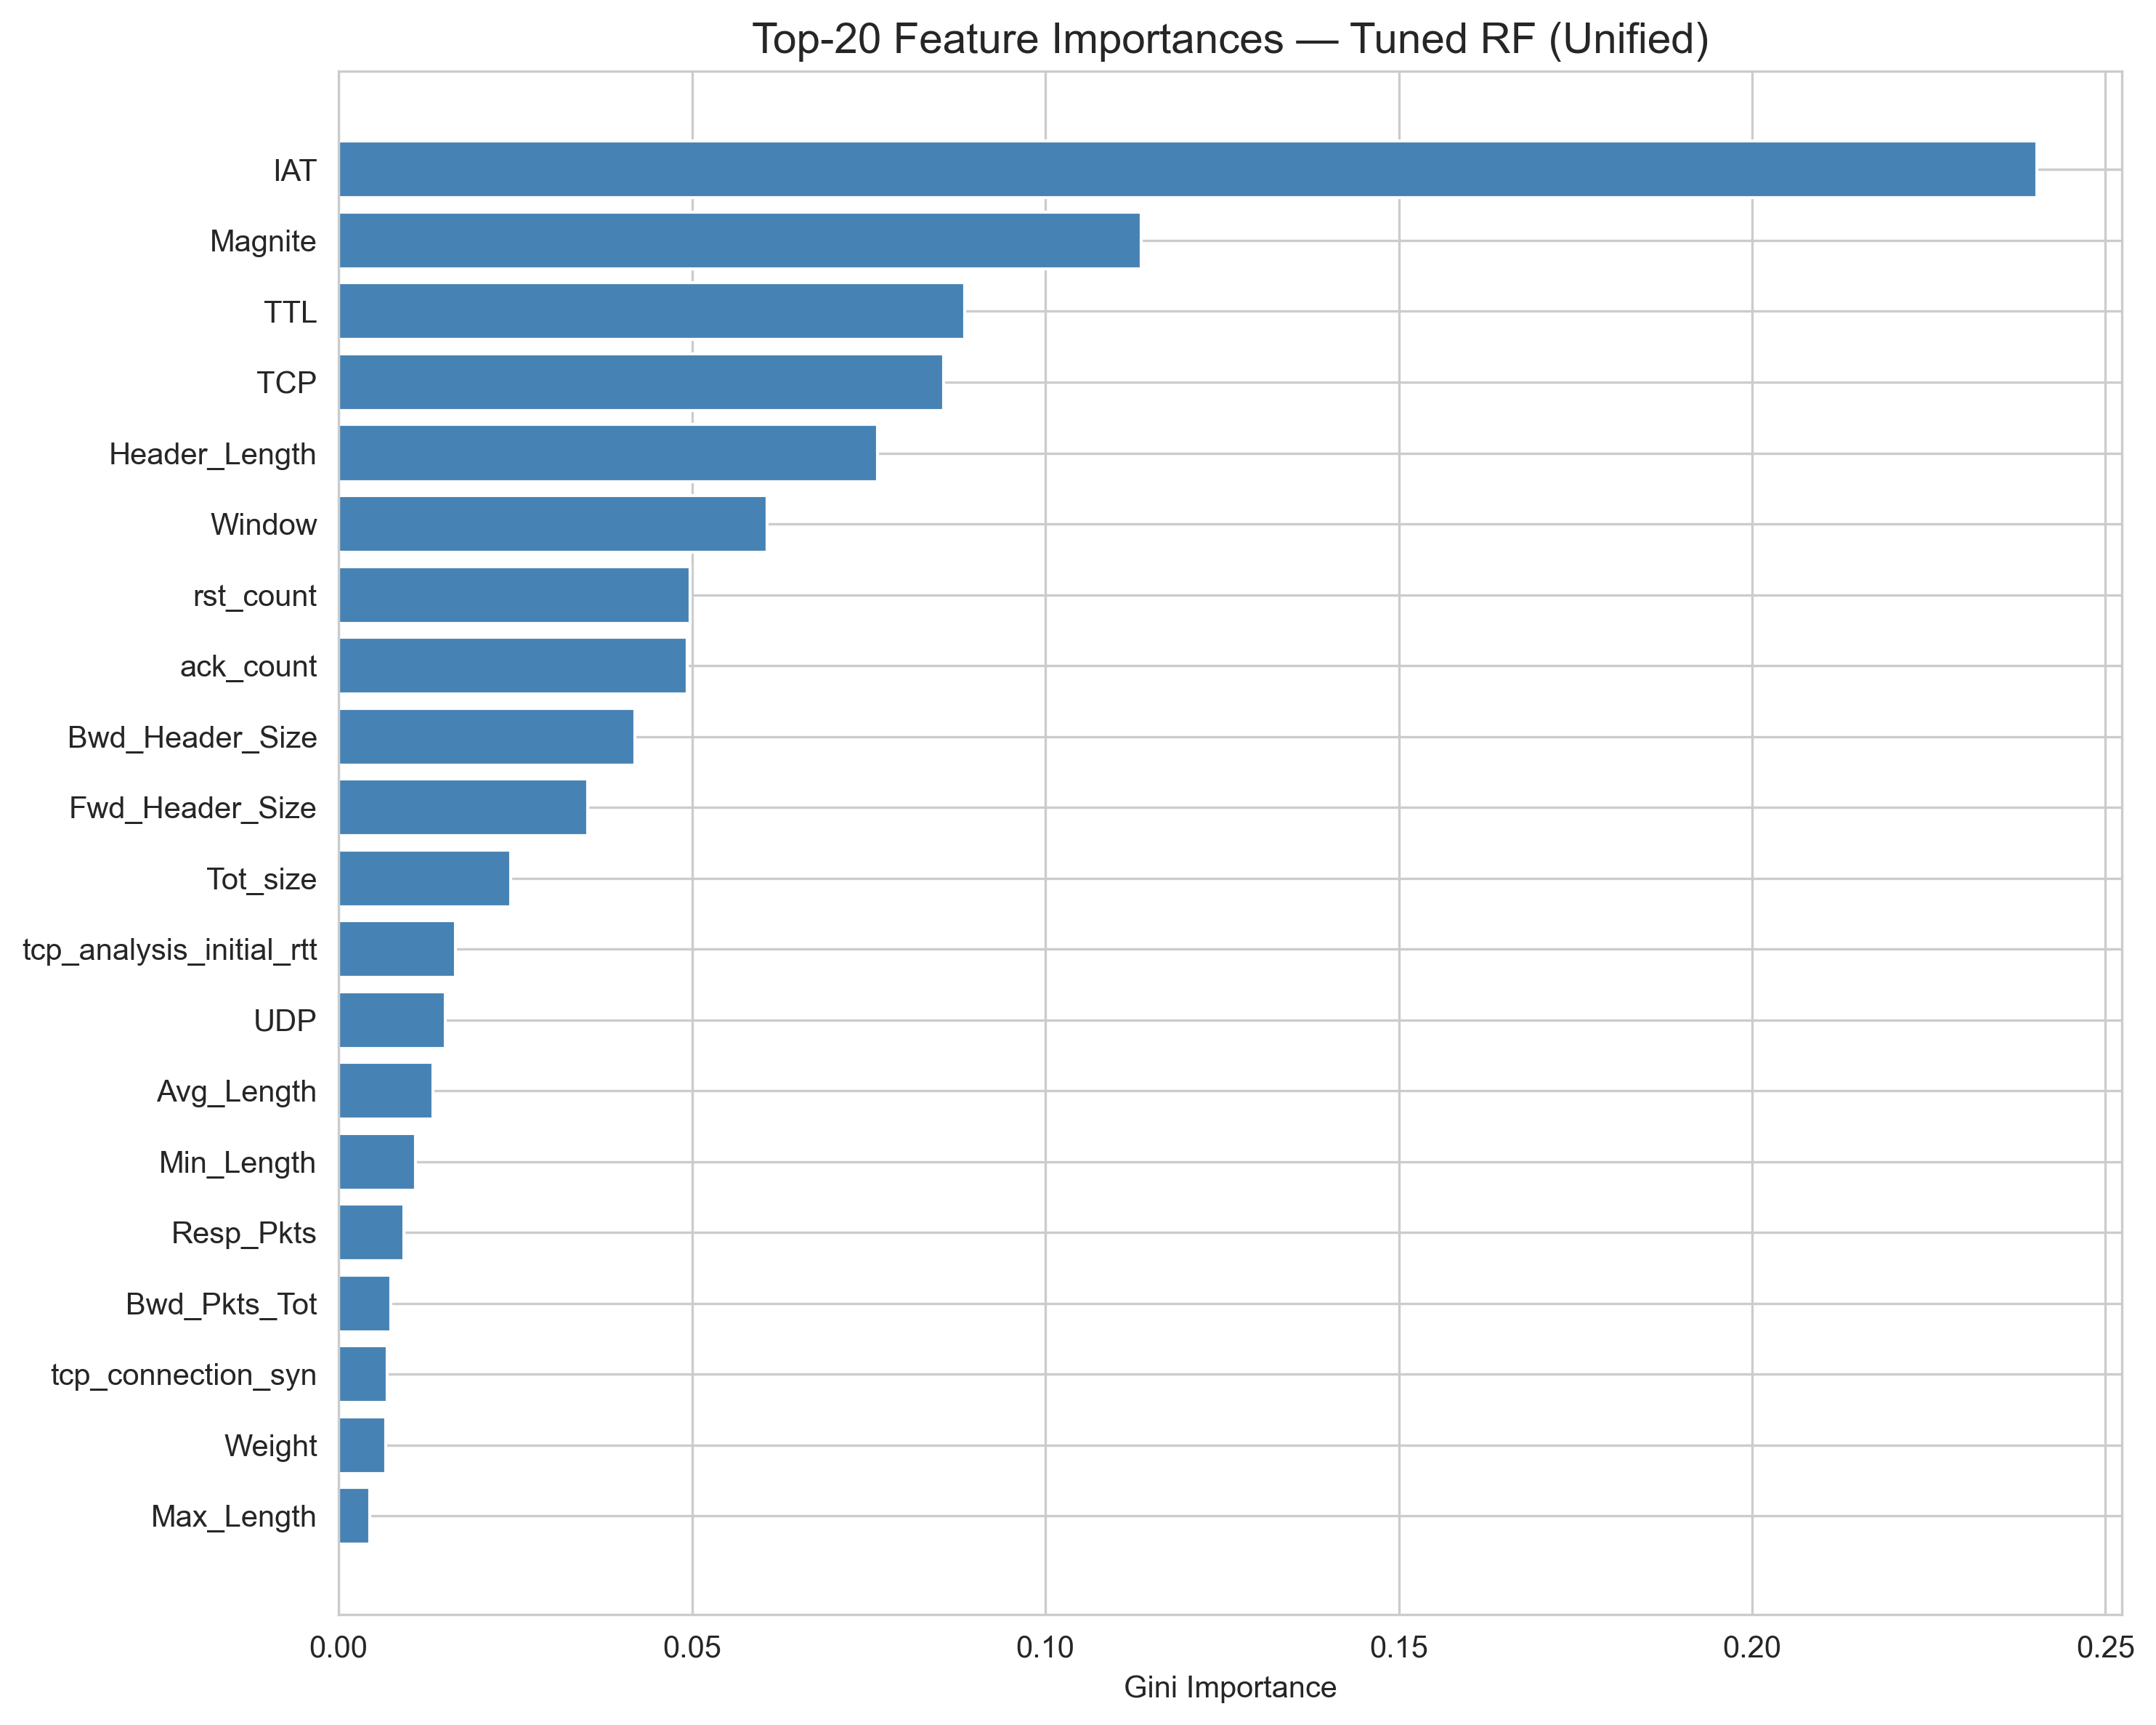
\includegraphics[width=0.85\textwidth]{ch5_rf_feature_importance_unified.png}
\caption{Top-20 feature importances for the tuned Random Forest (Unified regime).}
\label{fig:rf-feature-importance}
\end{figure}

\begin{figure}[H]
\centering
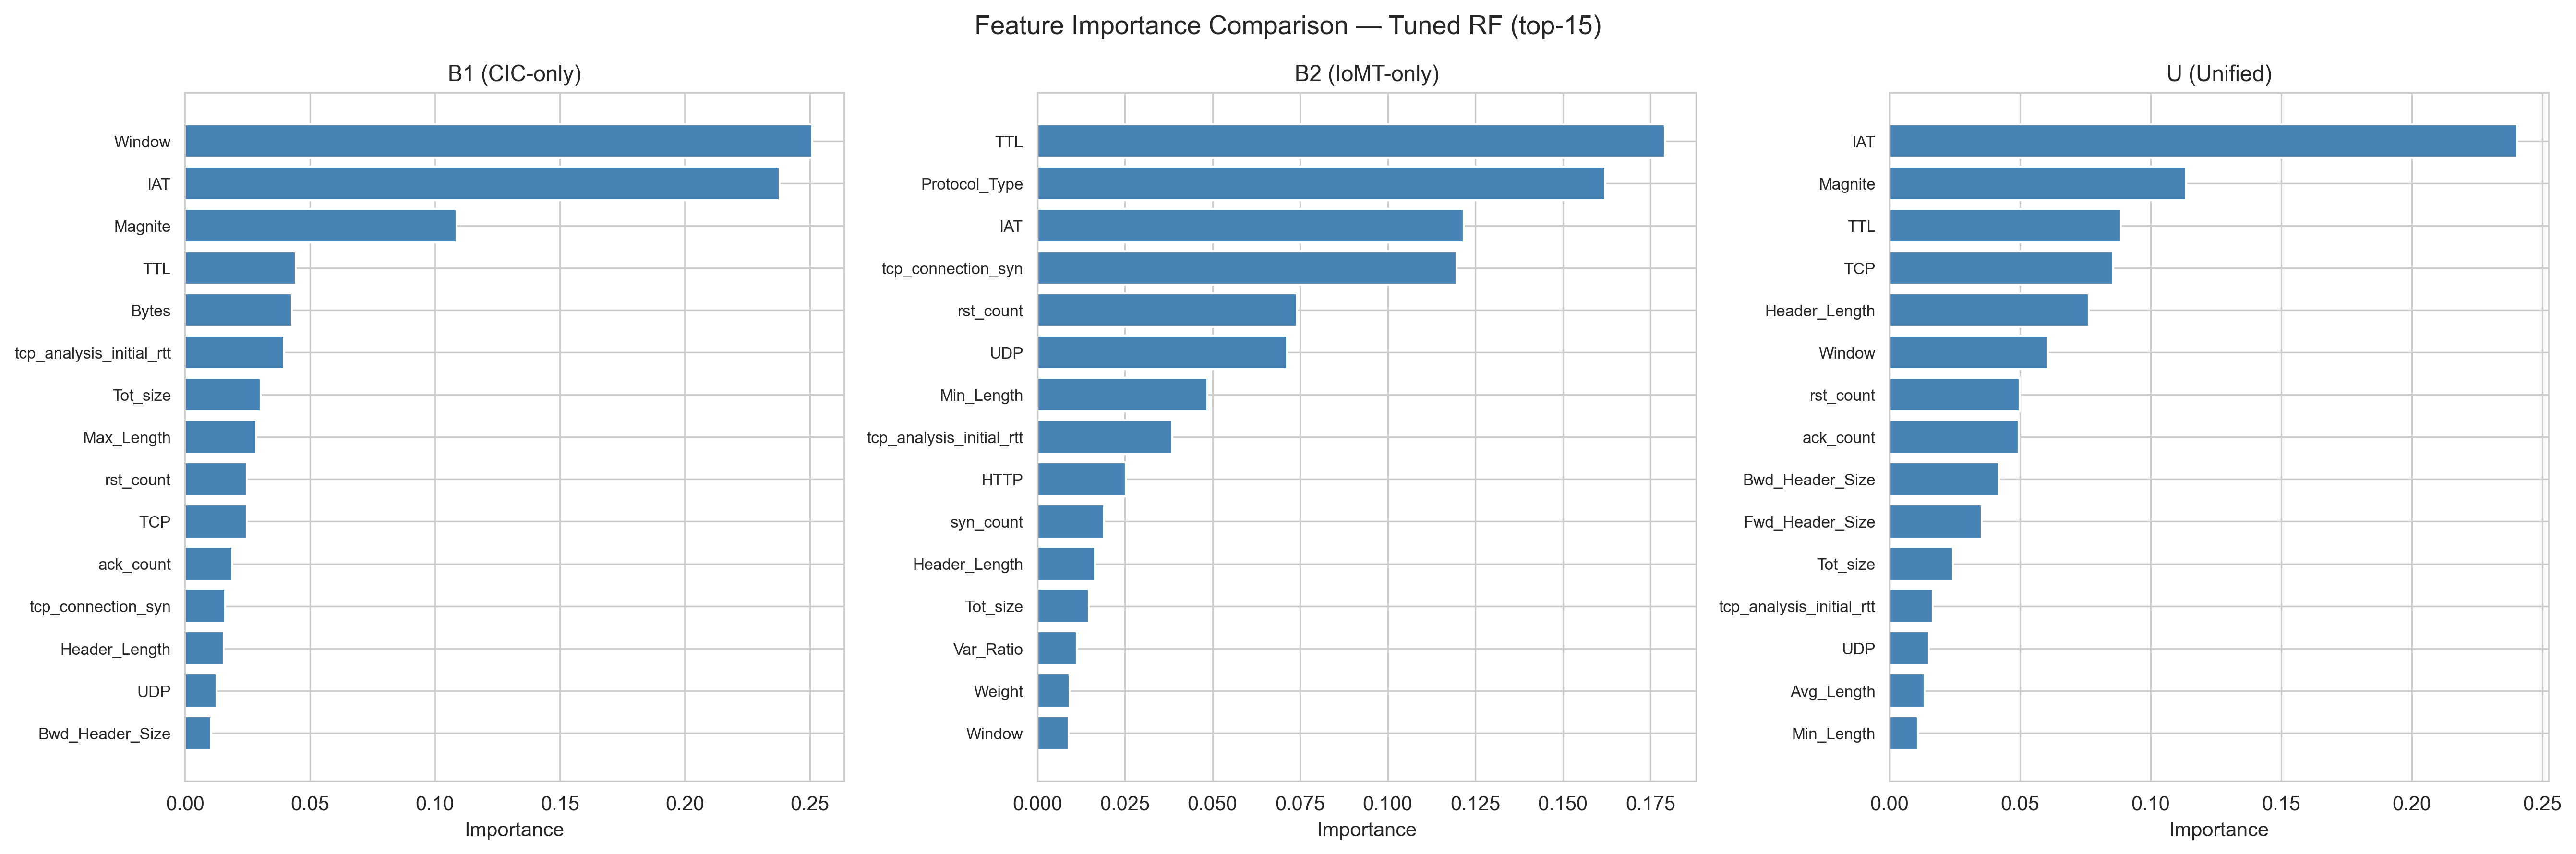
\includegraphics[width=\textwidth]{ch5_rf_feature_importance_comparison.png}
\caption{Feature importance comparison across regimes (tuned RF, top-15).}
\label{fig:rf-fi-comparison}
\end{figure}

\subsubsection{Per-Class Analysis}

Figure~\ref{fig:rf-per-class-f1} compares per-class F1 across tuned regimes on the full test set. Table~\ref{tab:rf-perclass-unified} gives the detailed report for Tuned U.

\begin{figure}[H]
\centering
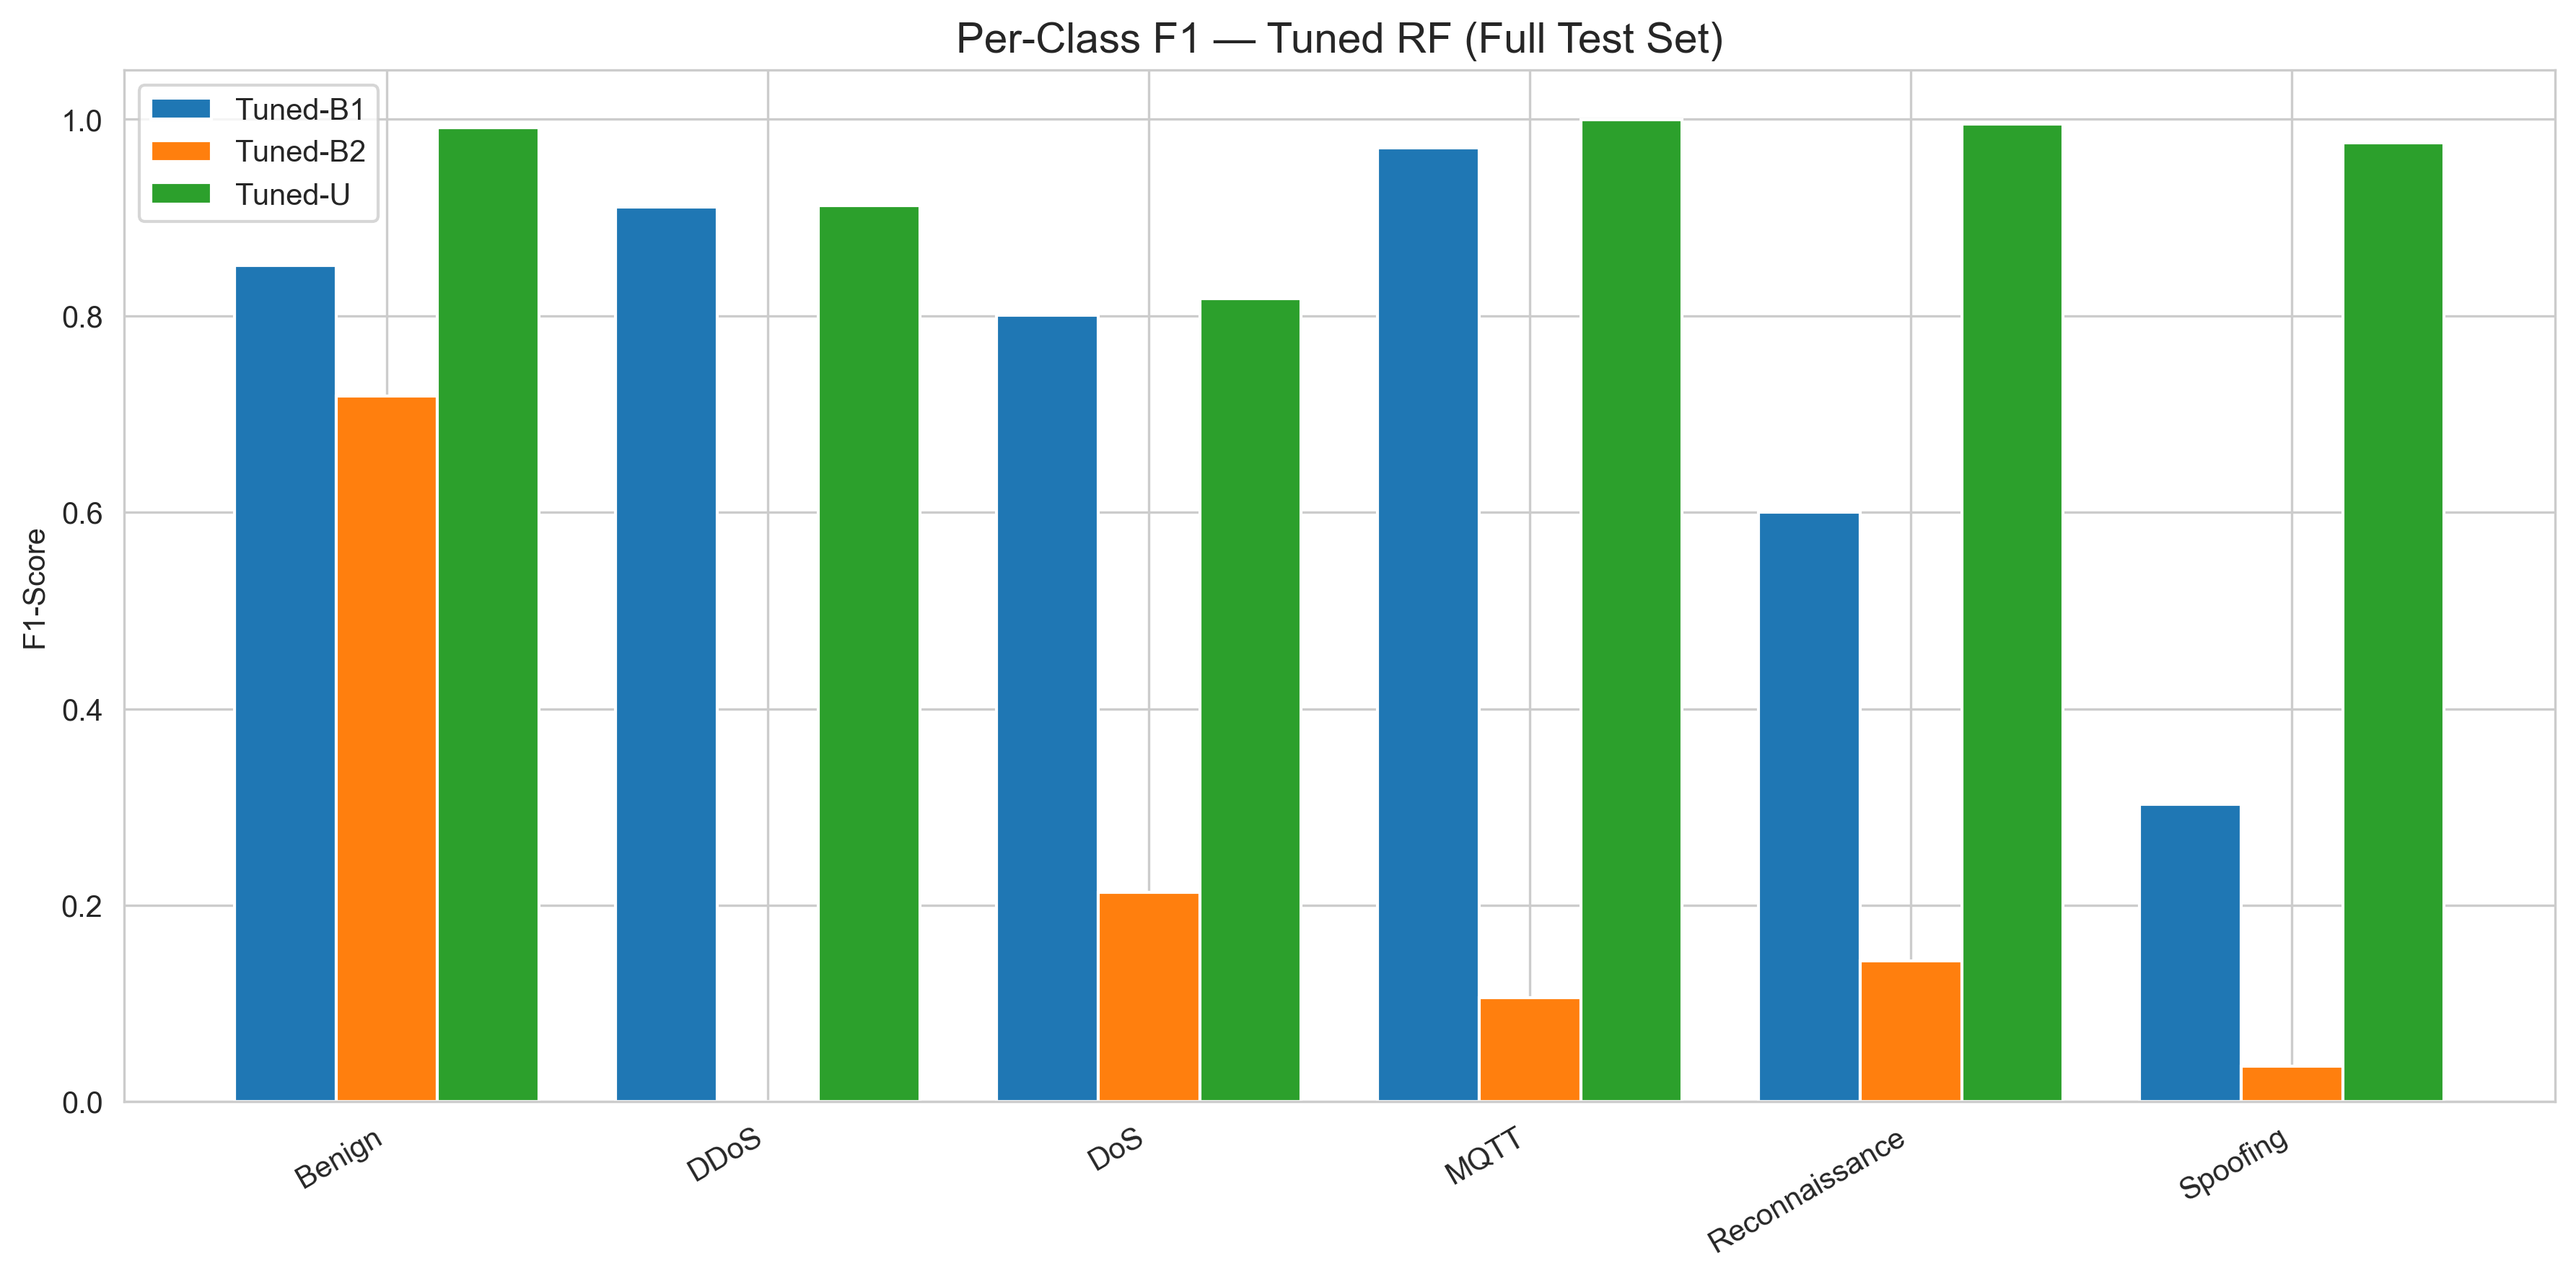
\includegraphics[width=0.85\textwidth]{ch5_rf_per_class_f1.png}
\caption{Per-class F1-score comparison across regimes (tuned RF, full test set).}
\label{fig:rf-per-class-f1}
\end{figure}

\begin{table}[H]
\centering
\caption{Per-class classification report for the tuned unified Random Forest on the full test set (1,201,731 samples).}
\label{tab:rf-perclass-unified}
\small
\begin{tabular}{@{}l r r r r@{}}
\toprule
\textbf{Class} & \textbf{Precision} & \textbf{Recall} & \textbf{F1-Score} & \textbf{Support} \\
\midrule
Benign          & 0.98 & 1.00 & 0.99 &     8,018 \\
DDoS            & 0.97 & 0.86 & 0.91 &   805,244 \\
DoS             & 0.73 & 0.93 & 0.82 &   322,273 \\
MQTT            & 1.00 & 1.00 & 1.00 &    57,891 \\
Reconnaissance  & 1.00 & 0.99 & 1.00 &     6,904 \\
Spoofing        & 0.97 & 0.99 & 0.98 &     1,401 \\
\midrule
Accuracy        &      &      & 0.89 & 1,201,731 \\
Macro avg       & 0.94 & 0.96 & 0.95 & 1,201,731 \\
Weighted avg    & 0.91 & 0.89 & 0.89 & 1,201,731 \\
\bottomrule
\end{tabular}
\end{table}

The Random Forest reproduces the same qualitative structure as the Decision Tree: near-perfect scores on Benign, MQTT, Reconnaissance, and Spoofing, with residual error concentrated in the DDoS/DoS boundary. Macro-F1 on the full test improves slightly relative to the tuned DT (0.9487 vs.\ 0.9480), while weighted-F1 and accuracy are essentially unchanged. Critically, the hypothesis that ensemble voting would substantially reduce the DDoS/DoS confusion is \textbf{not confirmed}: DDoS F1 (0.91) and DoS F1 (0.82) are identical to the tuned DT values, confirming that the source of the confusion is a feature-representation limitation that averaging over decorrelated trees cannot resolve on its own.

\subsubsection{Summary}

\begin{itemize}[nosep]
  \item \textbf{Single-source models remain brittle cross-domain.} Tuned B1 improves IoMT Macro-F1 versus the DT baseline (0.34 vs.\ 0.25) but still fails to generalize. Tuned B2 collapses on the full and CIC slices for the same structural reason as before (no DDoS exposure).
  \item \textbf{Unified RF matches or marginally exceeds unified DT.} Full-test Macro-F1 reaches 0.9487 (+0.7 percentage points over tuned DT). Cross-domain slices for Tuned U remain strong (CIC 0.9285, IoMT 0.8329 before the absent-class caveat above).
  \item \textbf{Ensemble variance reduction.} The selected shallow trees with \texttt{max\_samples}=0.8 and moderate \texttt{n\_estimators} (200--300) provide a stable bias--variance trade-off without the extreme memory cost of very large unrestricted forests.
  \item \textbf{DDoS/DoS boundary: hypothesis not confirmed.} Despite the theoretical expectation that ensemble voting would smooth the DDoS$\leftrightarrow$DoS decision boundary, per-class F1 scores for both classes are indistinguishable from the Decision Tree (DDoS: 0.91, DoS: 0.82 in both cases). This null result reinforces that the boundary confusion is driven by absent multi-source diversity features in the current 58-feature window representation, not by model capacity.
\end{itemize}

\subsection{XGBoost Classifier}
\label{subsec:xgboost}

Gradient boosted trees (XGBoost) provide a third point on the bias--variance spectrum. Training uses histogram-based tree construction (\texttt{tree\_method='hist'}) and per-sample weights for class imbalance. Because the IoMT-only regime (B2) lacks the global DDoS class in its training partition, the implementation remaps the present global label indices to contiguous integers during XGBoost's \texttt{multi:softmax} fit and maps predictions back to the global six-class space for evaluation---mirroring how the encoder still defines a common confusion-matrix layout.

\subsubsection{Baseline Results}

Table~\ref{tab:xgb-baseline} reports baseline XGBoost performance ($n_{\text{estimators}}=100$, default learning rate).

\begin{table}[H]
\centering
\caption{Baseline XGBoost evaluation matrix.}
\label{tab:xgb-baseline}
\small
\begin{tabular}{@{}l l c c c@{}}
\toprule
\textbf{Regime} & \textbf{Test slice} & \textbf{Macro-F1} & \textbf{Weighted-F1} & \textbf{Accuracy} \\
\midrule
B1 (CIC-only) & CIC (in-domain)  & 0.9376 & 0.8923 & 0.8888 \\
B1 (CIC-only) & IoMT (cross)     & 0.3576 & 0.5052 & 0.5238 \\
B1 (CIC-only) & Full             & 0.7629 & 0.8834 & 0.8804 \\
\midrule
B2 (IoMT-only) & IoMT (in-domain) & 0.8333 & 0.9999 & 0.9999 \\
B2 (IoMT-only) & CIC (cross)      & 0.0900 & 0.0862 & 0.1061 \\
B2 (IoMT-only) & Full             & 0.3602 & 0.0990 & 0.1266 \\
\midrule
U (Unified)    & CIC              & 0.9380 & 0.8924 & 0.8889 \\
U (Unified)    & IoMT             & 0.8333 & 1.0000 & 1.0000 \\
U (Unified)    & Full             & \textbf{0.9520} & 0.8947 & 0.8914 \\
\bottomrule
\end{tabular}
\end{table}

\subsubsection{Tuned Results}

Table~\ref{tab:xgb-tuned} reports tuned XGBoost results. Table~\ref{tab:xgb-best-params} lists the best hyperparameters (CV macro-F1 on the search subsample / full B2 training set).

\begin{table}[H]
\centering
\caption{Tuned XGBoost evaluation matrix.}
\label{tab:xgb-tuned}
\small
\begin{tabular}{@{}l l c c c@{}}
\toprule
\textbf{Regime} & \textbf{Test slice} & \textbf{Macro-F1} & \textbf{Weighted-F1} & \textbf{Accuracy} \\
\midrule
Tuned B1 & CIC (in-domain)  & 0.9410 & 0.8951 & 0.8918 \\
Tuned B1 & IoMT (cross)     & 0.2724 & 0.4057 & 0.4394 \\
Tuned B1 & Full             & 0.7199 & 0.8838 & 0.8814 \\
\midrule
Tuned B2 & IoMT (in-domain) & 0.8333 & 1.0000 & 1.0000 \\
Tuned B2 & CIC (cross)      & 0.1079 & 0.1045 & 0.1810 \\
Tuned B2 & Full             & 0.3708 & 0.1161 & 0.1998 \\
\midrule
Tuned U  & CIC              & 0.9382 & 0.8931 & 0.8897 \\
Tuned U  & IoMT             & 0.8333 & 0.9999 & 0.9999 \\
Tuned U  & Full             & \textbf{0.9522} & 0.8954 & 0.8922 \\
\bottomrule
\end{tabular}
\end{table}

\paragraph{Note on Macro-F1 (IoMT slice, Tuned U).}
The same absent-class effect as in Tables~\ref{tab:dt-tuned} and~\ref{tab:rf-tuned} applies: IoMT test traffic carries no DDoS label, so the global Macro-F1 on that slice (0.8333) averages over a zero-score DDoS column.

\begin{table}[H]
\centering
\caption{Best hyperparameters per regime (XGBoost, 50-iteration RandomizedSearchCV). Abbreviations: mcw $=$ \texttt{min\_child\_weight}, cbt $=$ \texttt{colsample\_bytree}, $\lambda$ $=$ \texttt{reg\_lambda}, $\alpha$ $=$ \texttt{reg\_alpha}.}
\label{tab:xgb-best-params}
\scriptsize
\begin{tabular}{@{}l c c c c c c c c c c@{}}
\toprule
\textbf{Reg.} & \textbf{lr} & \textbf{trees} & \textbf{depth} & \textbf{mcw} & \textbf{subs.} & \textbf{cbt} & $\gamma$ & $\lambda$ & $\alpha$ & \textbf{CV F1m} \\
\midrule
B1 & 0.10 & 500 & 12 & 20 & 0.6 & 0.9 & 0.1 & 1 & 0.1 & 0.9437 \\
B2 & 0.20 & 200 & 12 & 1  & 0.9 & 0.8 & 0 & 0.01 & 1 & 0.9999 \\
U  & 0.03 & 500 & 9  & 5  & 0.6 & 0.9 & 0 & 0.01 & 0 & 0.9575 \\
\bottomrule
\end{tabular}
\end{table}

\subsubsection{Cross-Domain Analysis}

Figure~\ref{fig:xgb-confusion-unified} shows the normalized confusion matrix for the tuned unified XGBoost on the full test set. Figure~\ref{fig:xgb-cm-xd} shows the cross-domain matrices for B1$\to$IoMT and B2$\to$CIC.

\begin{figure}[H]
\centering
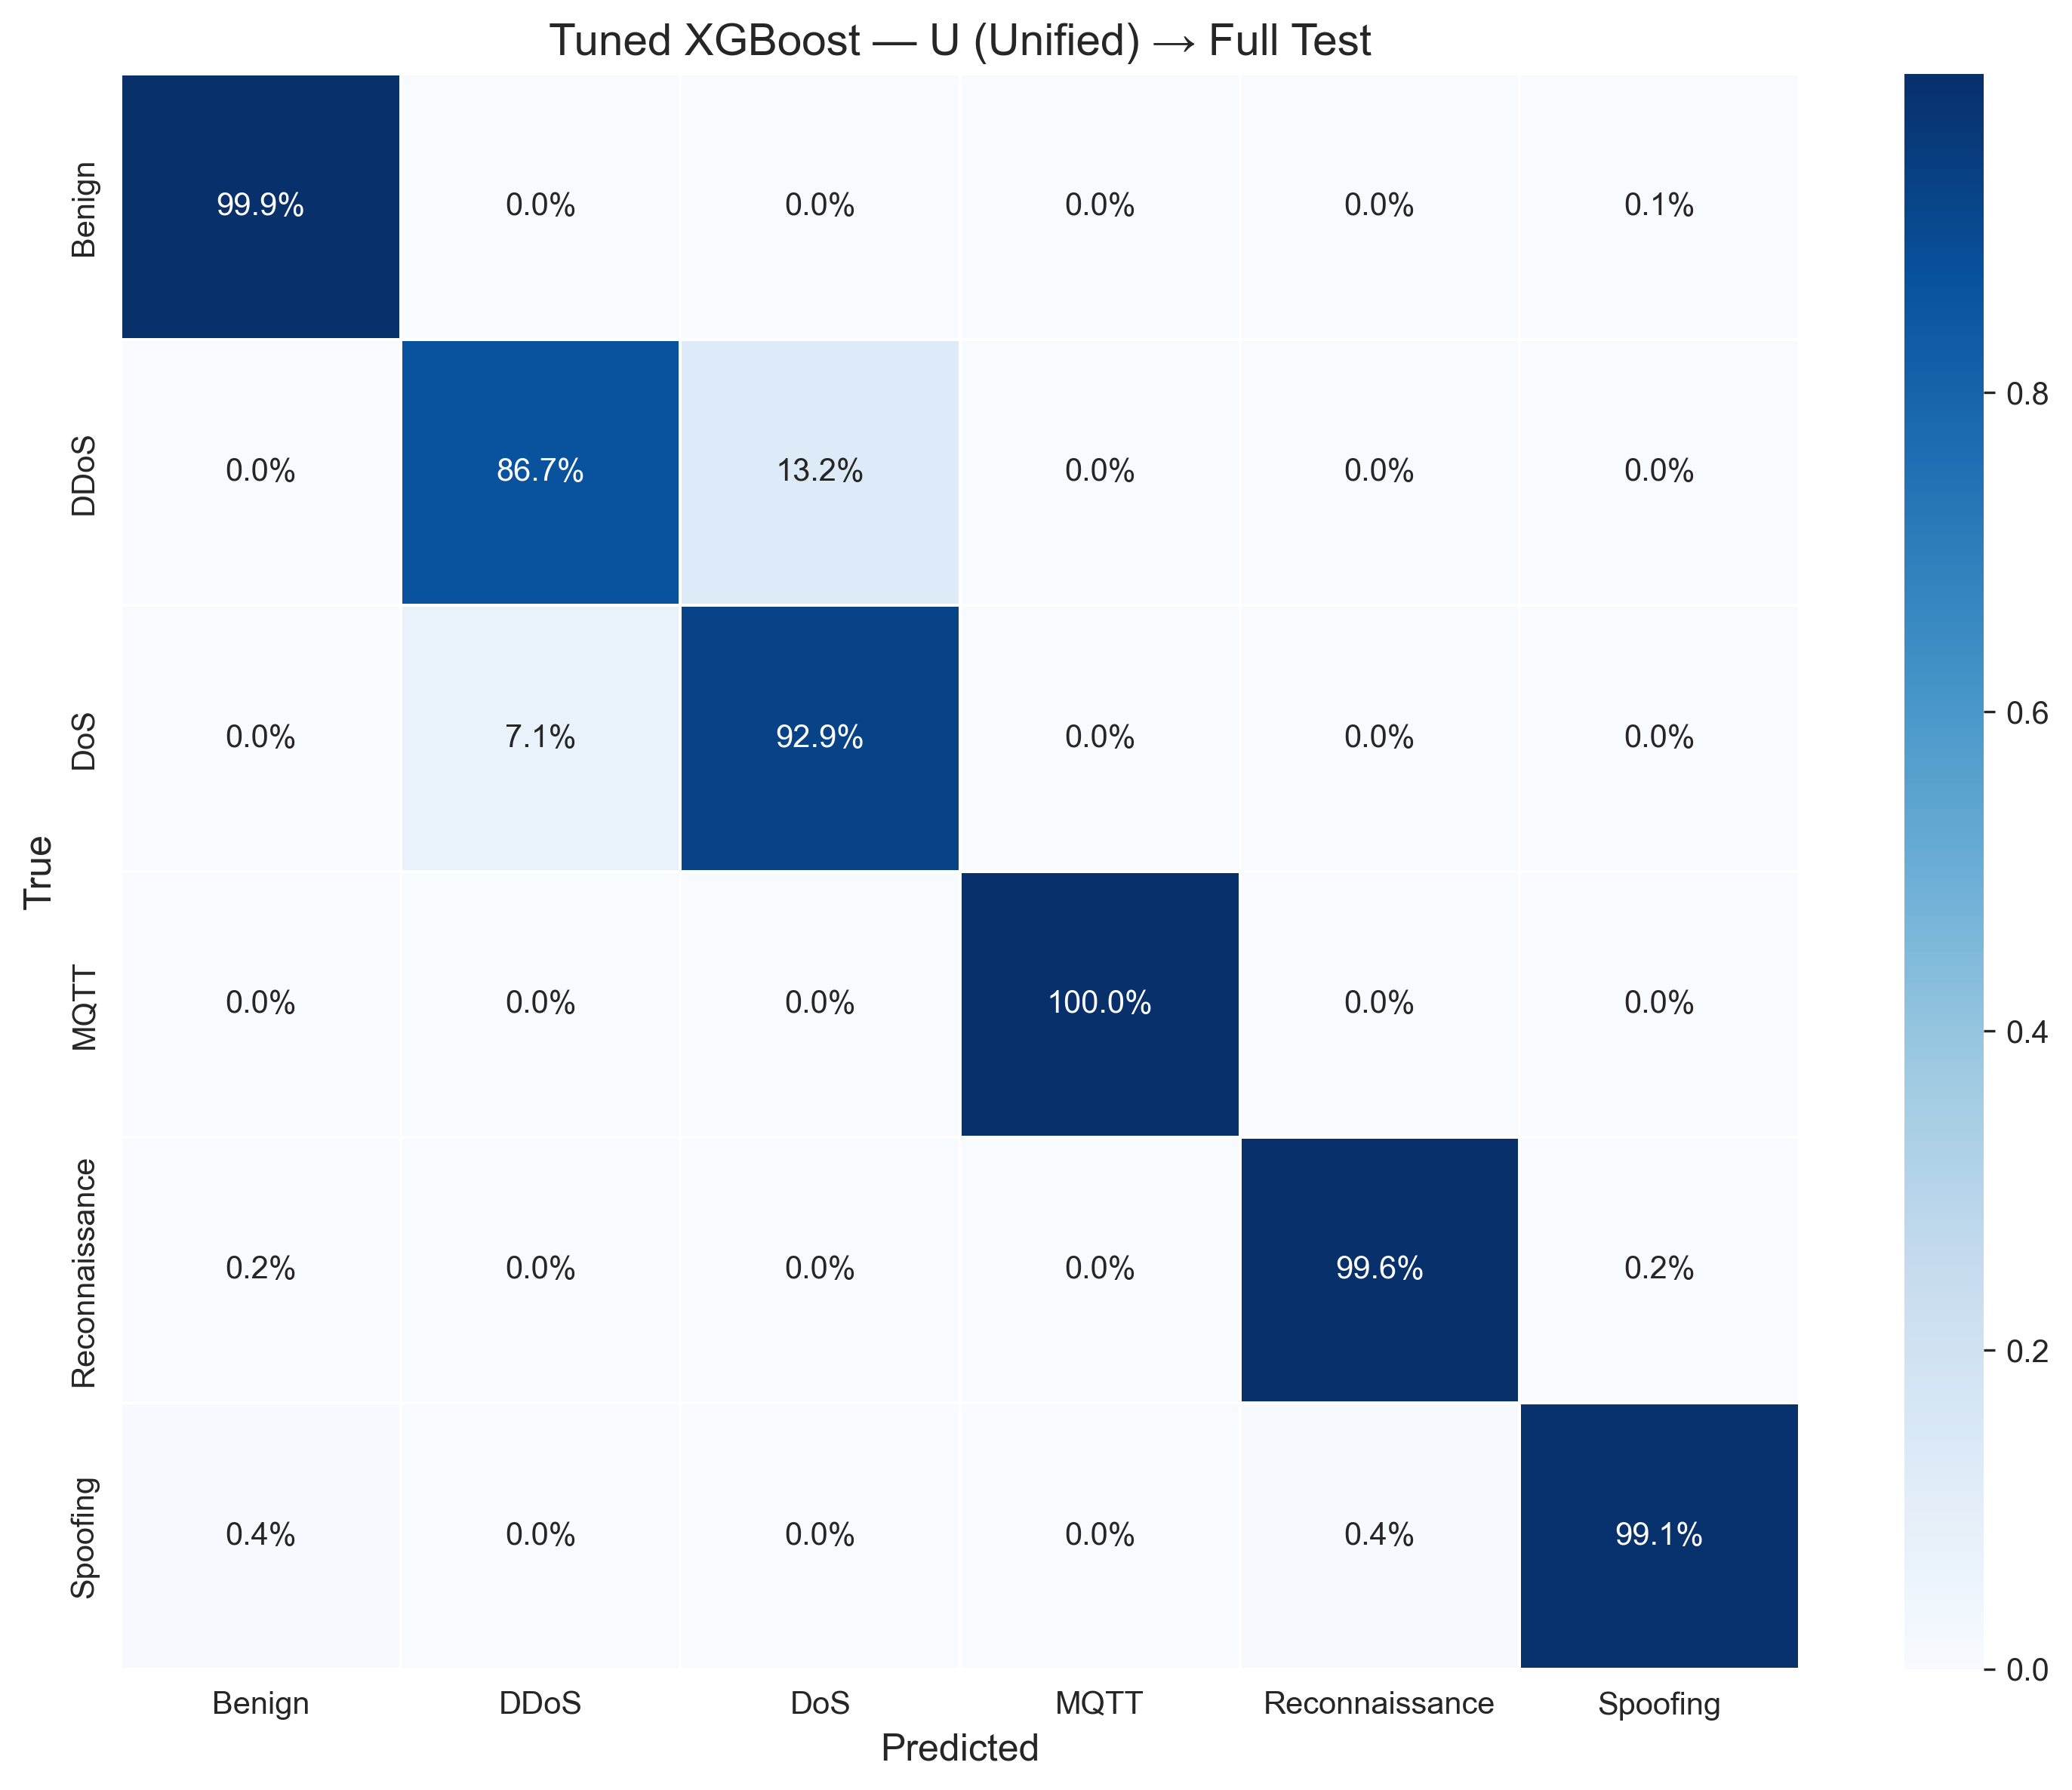
\includegraphics[width=0.75\textwidth]{ch5_xgb_cm_u_full.png}
\caption{Normalized confusion matrix --- Tuned XGBoost (Unified) on the full test set.}
\label{fig:xgb-confusion-unified}
\end{figure}

\begin{figure}[H]
\centering
\begin{subfigure}[b]{0.48\textwidth}
  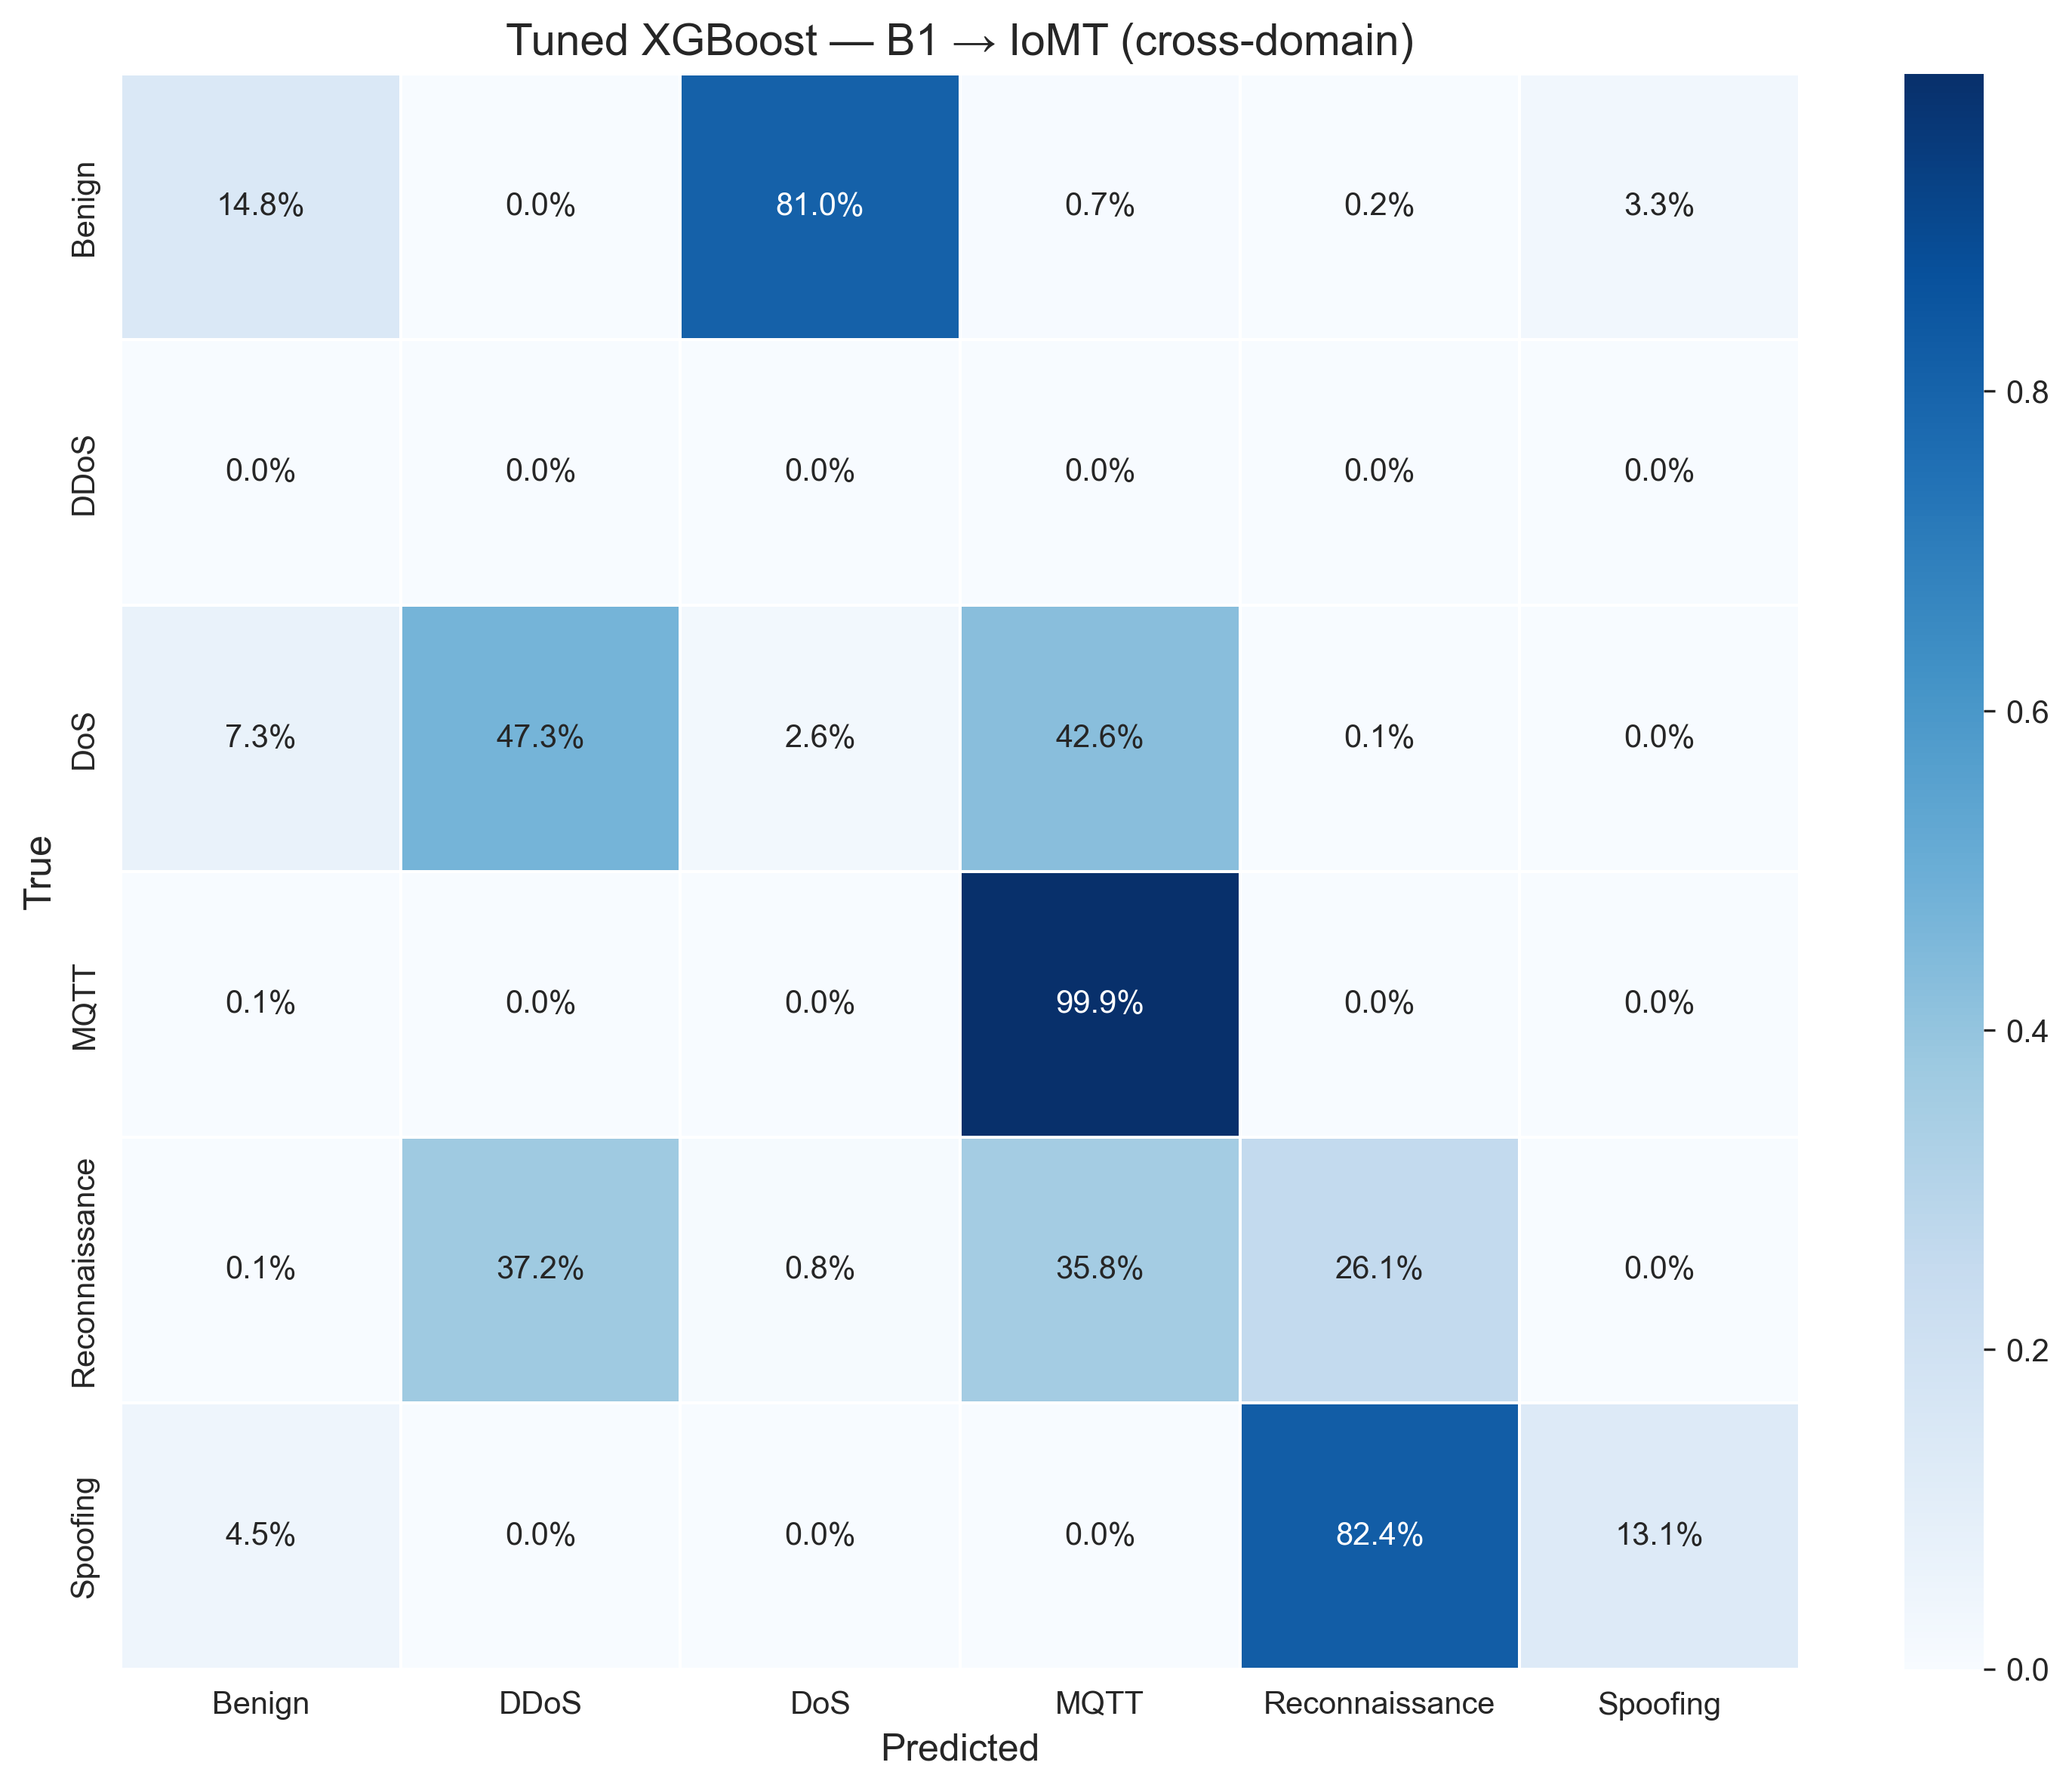
\includegraphics[width=\textwidth]{ch5_xgb_cm_b1_xd_iomt.png}
  \caption{B1 (CIC-only) $\to$ IoMT test}
\end{subfigure}
\hfill
\begin{subfigure}[b]{0.48\textwidth}
  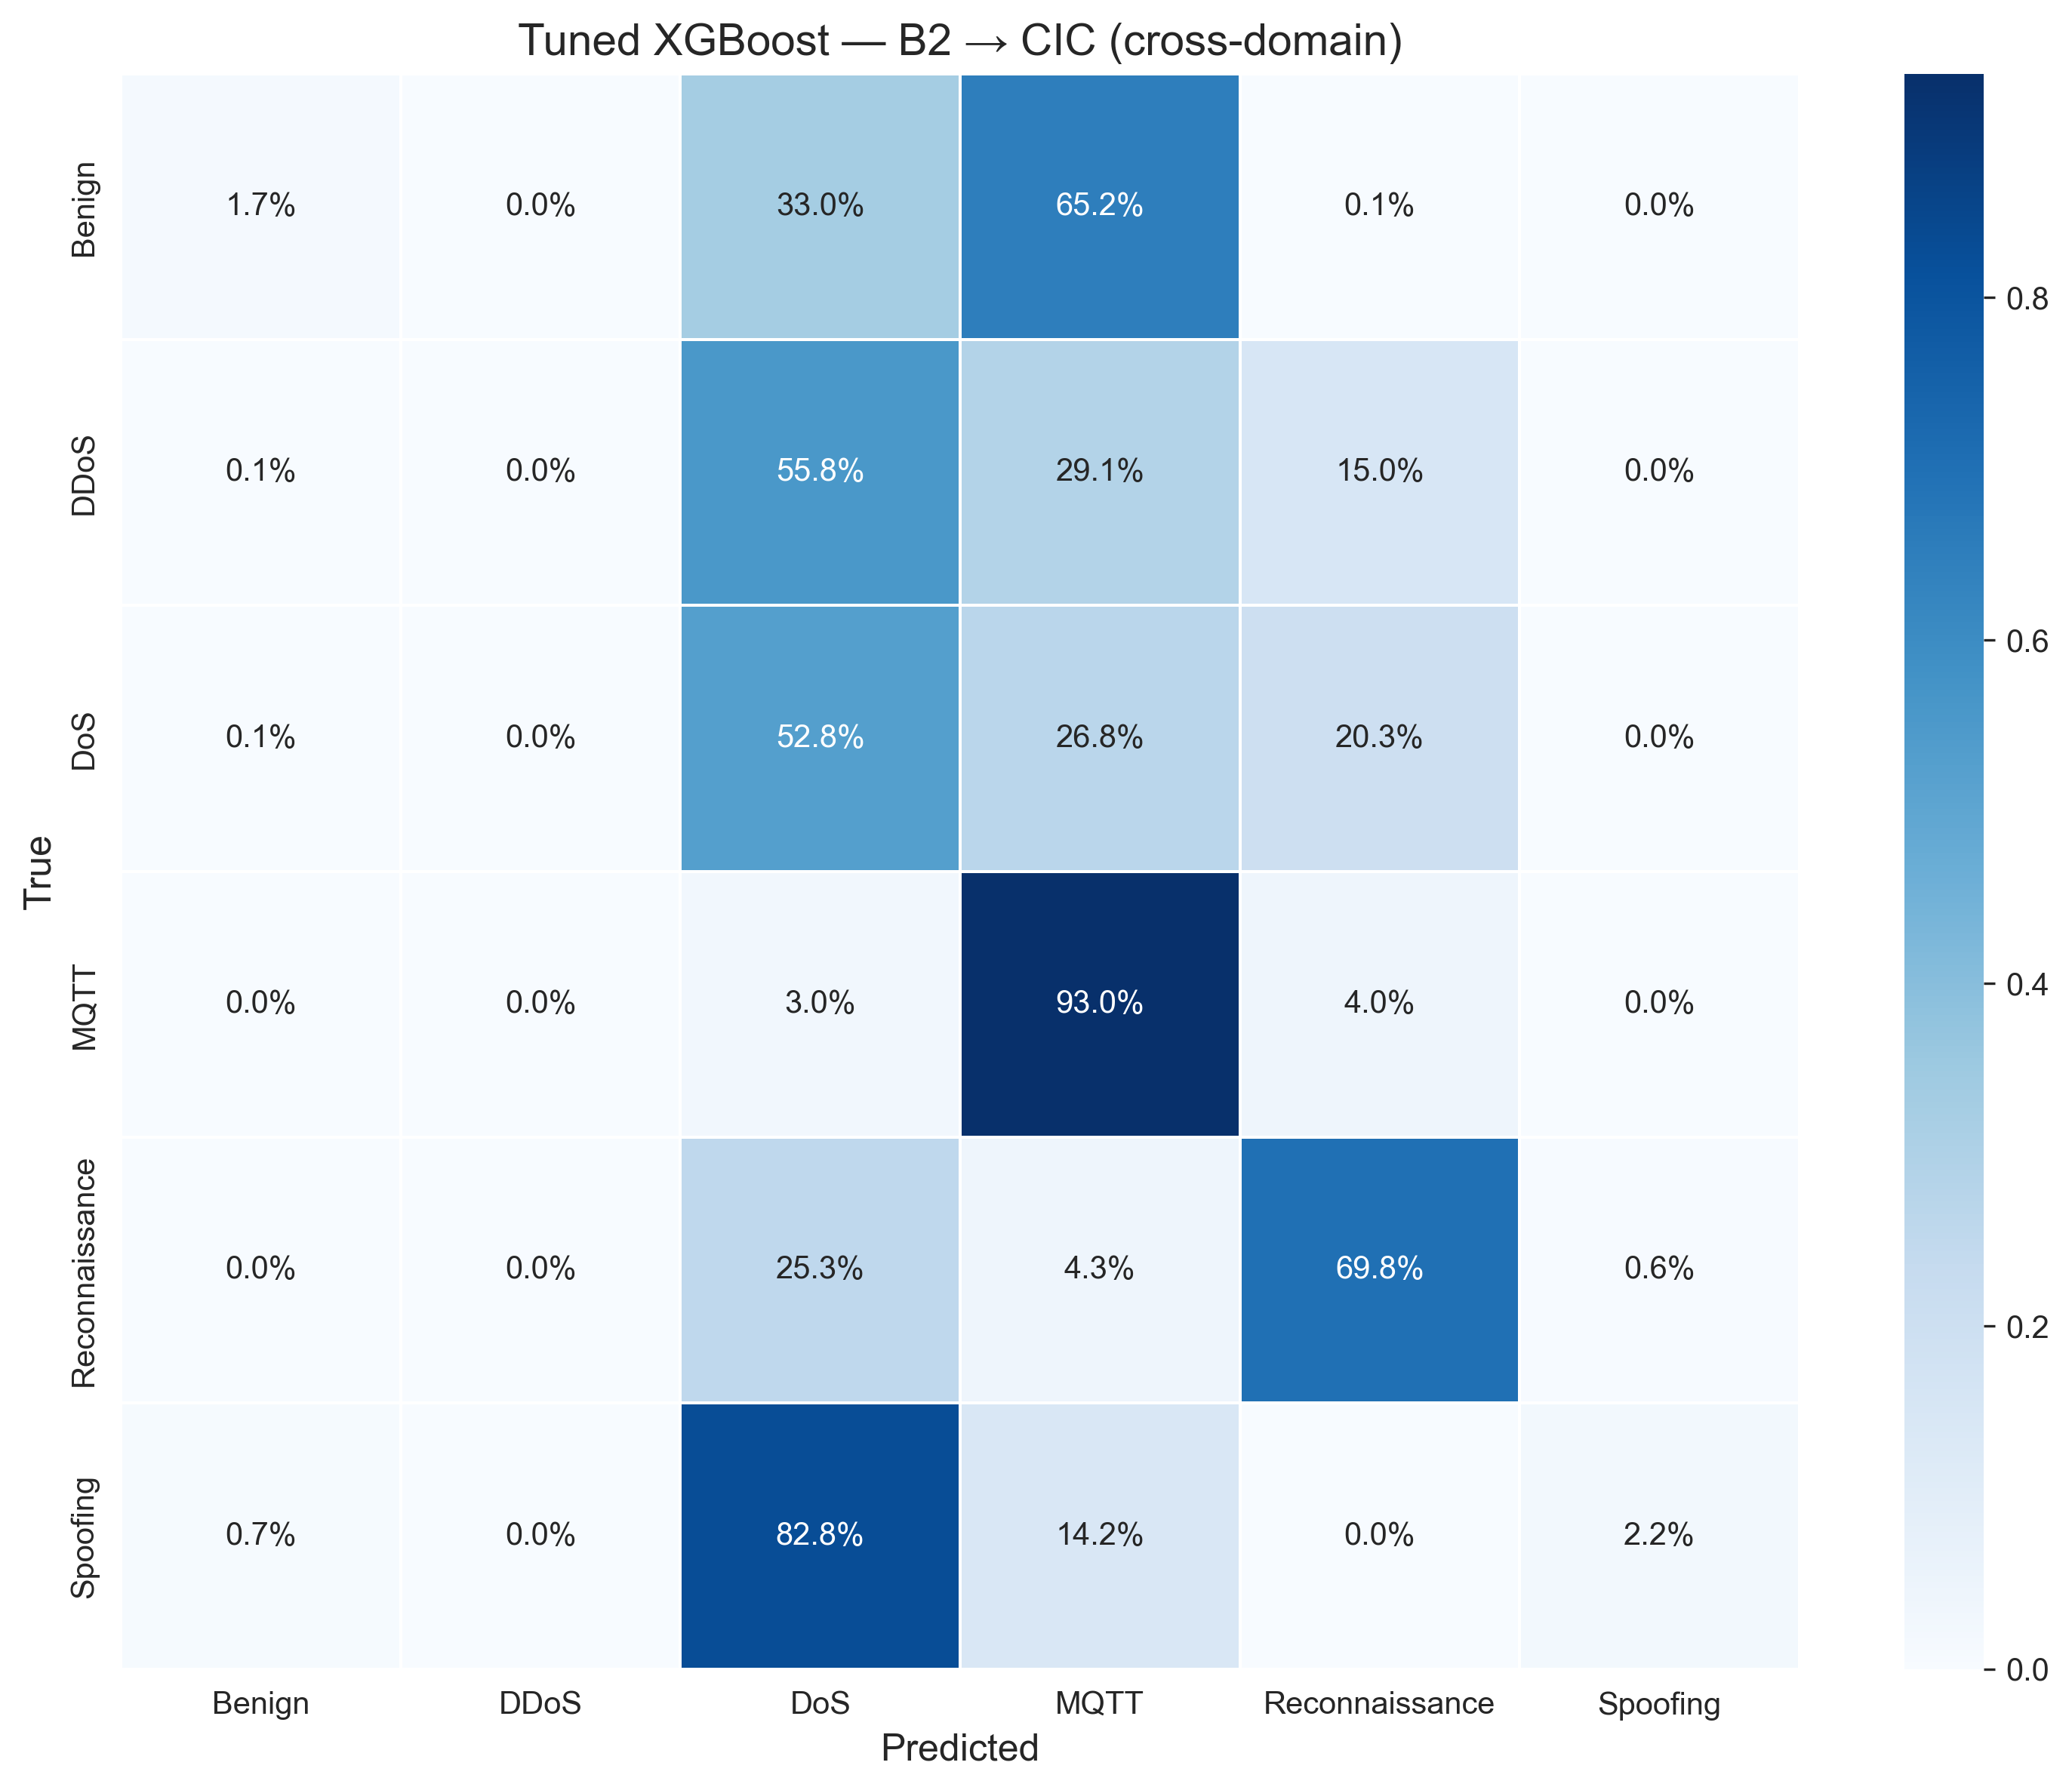
\includegraphics[width=\textwidth]{ch5_xgb_cm_b2_xd_cic.png}
  \caption{B2 (IoMT-only) $\to$ CIC test}
\end{subfigure}
\caption{Cross-domain confusion matrices for tuned XGBoost models.}
\label{fig:xgb-cm-xd}
\end{figure}

The unified XGBoost confusion matrix (Figure~\ref{fig:xgb-confusion-unified}) reproduces the same dominant DDoS$\leftrightarrow$DoS error pattern observed for DT and RF, with all other class pairs near-zero error. The B1$\to$IoMT cross-domain score (Macro-F1 = 0.2724) is lower than the Random Forest equivalent (0.3423), likely because the XGBoost hyperparameters were tuned on a 300k-row subsample of the CIC training data, which may have introduced a tighter fit to the CIC distribution and reduced out-of-distribution generalization. The B2$\to$CIC slice (0.1079) remains poor for the structural reason shared by all three classifiers: DDoS traffic is entirely absent from the B2 training partition, making it impossible for any model in that regime to produce correct predictions on the DDoS-dominated CIC test slice.

\subsubsection{Feature Importance}

Figure~\ref{fig:xgb-feature-importance} shows the top-20 gain-based feature importances for the tuned unified XGBoost model, and Figure~\ref{fig:xgb-fi-comparison} compares importance rankings across all three regimes (top-15). XGBoost's gain importance reflects the average improvement in the loss function per split on a given feature, providing a complementary perspective to the Gini importance used by Decision Tree and Random Forest.

\begin{figure}[H]
\centering
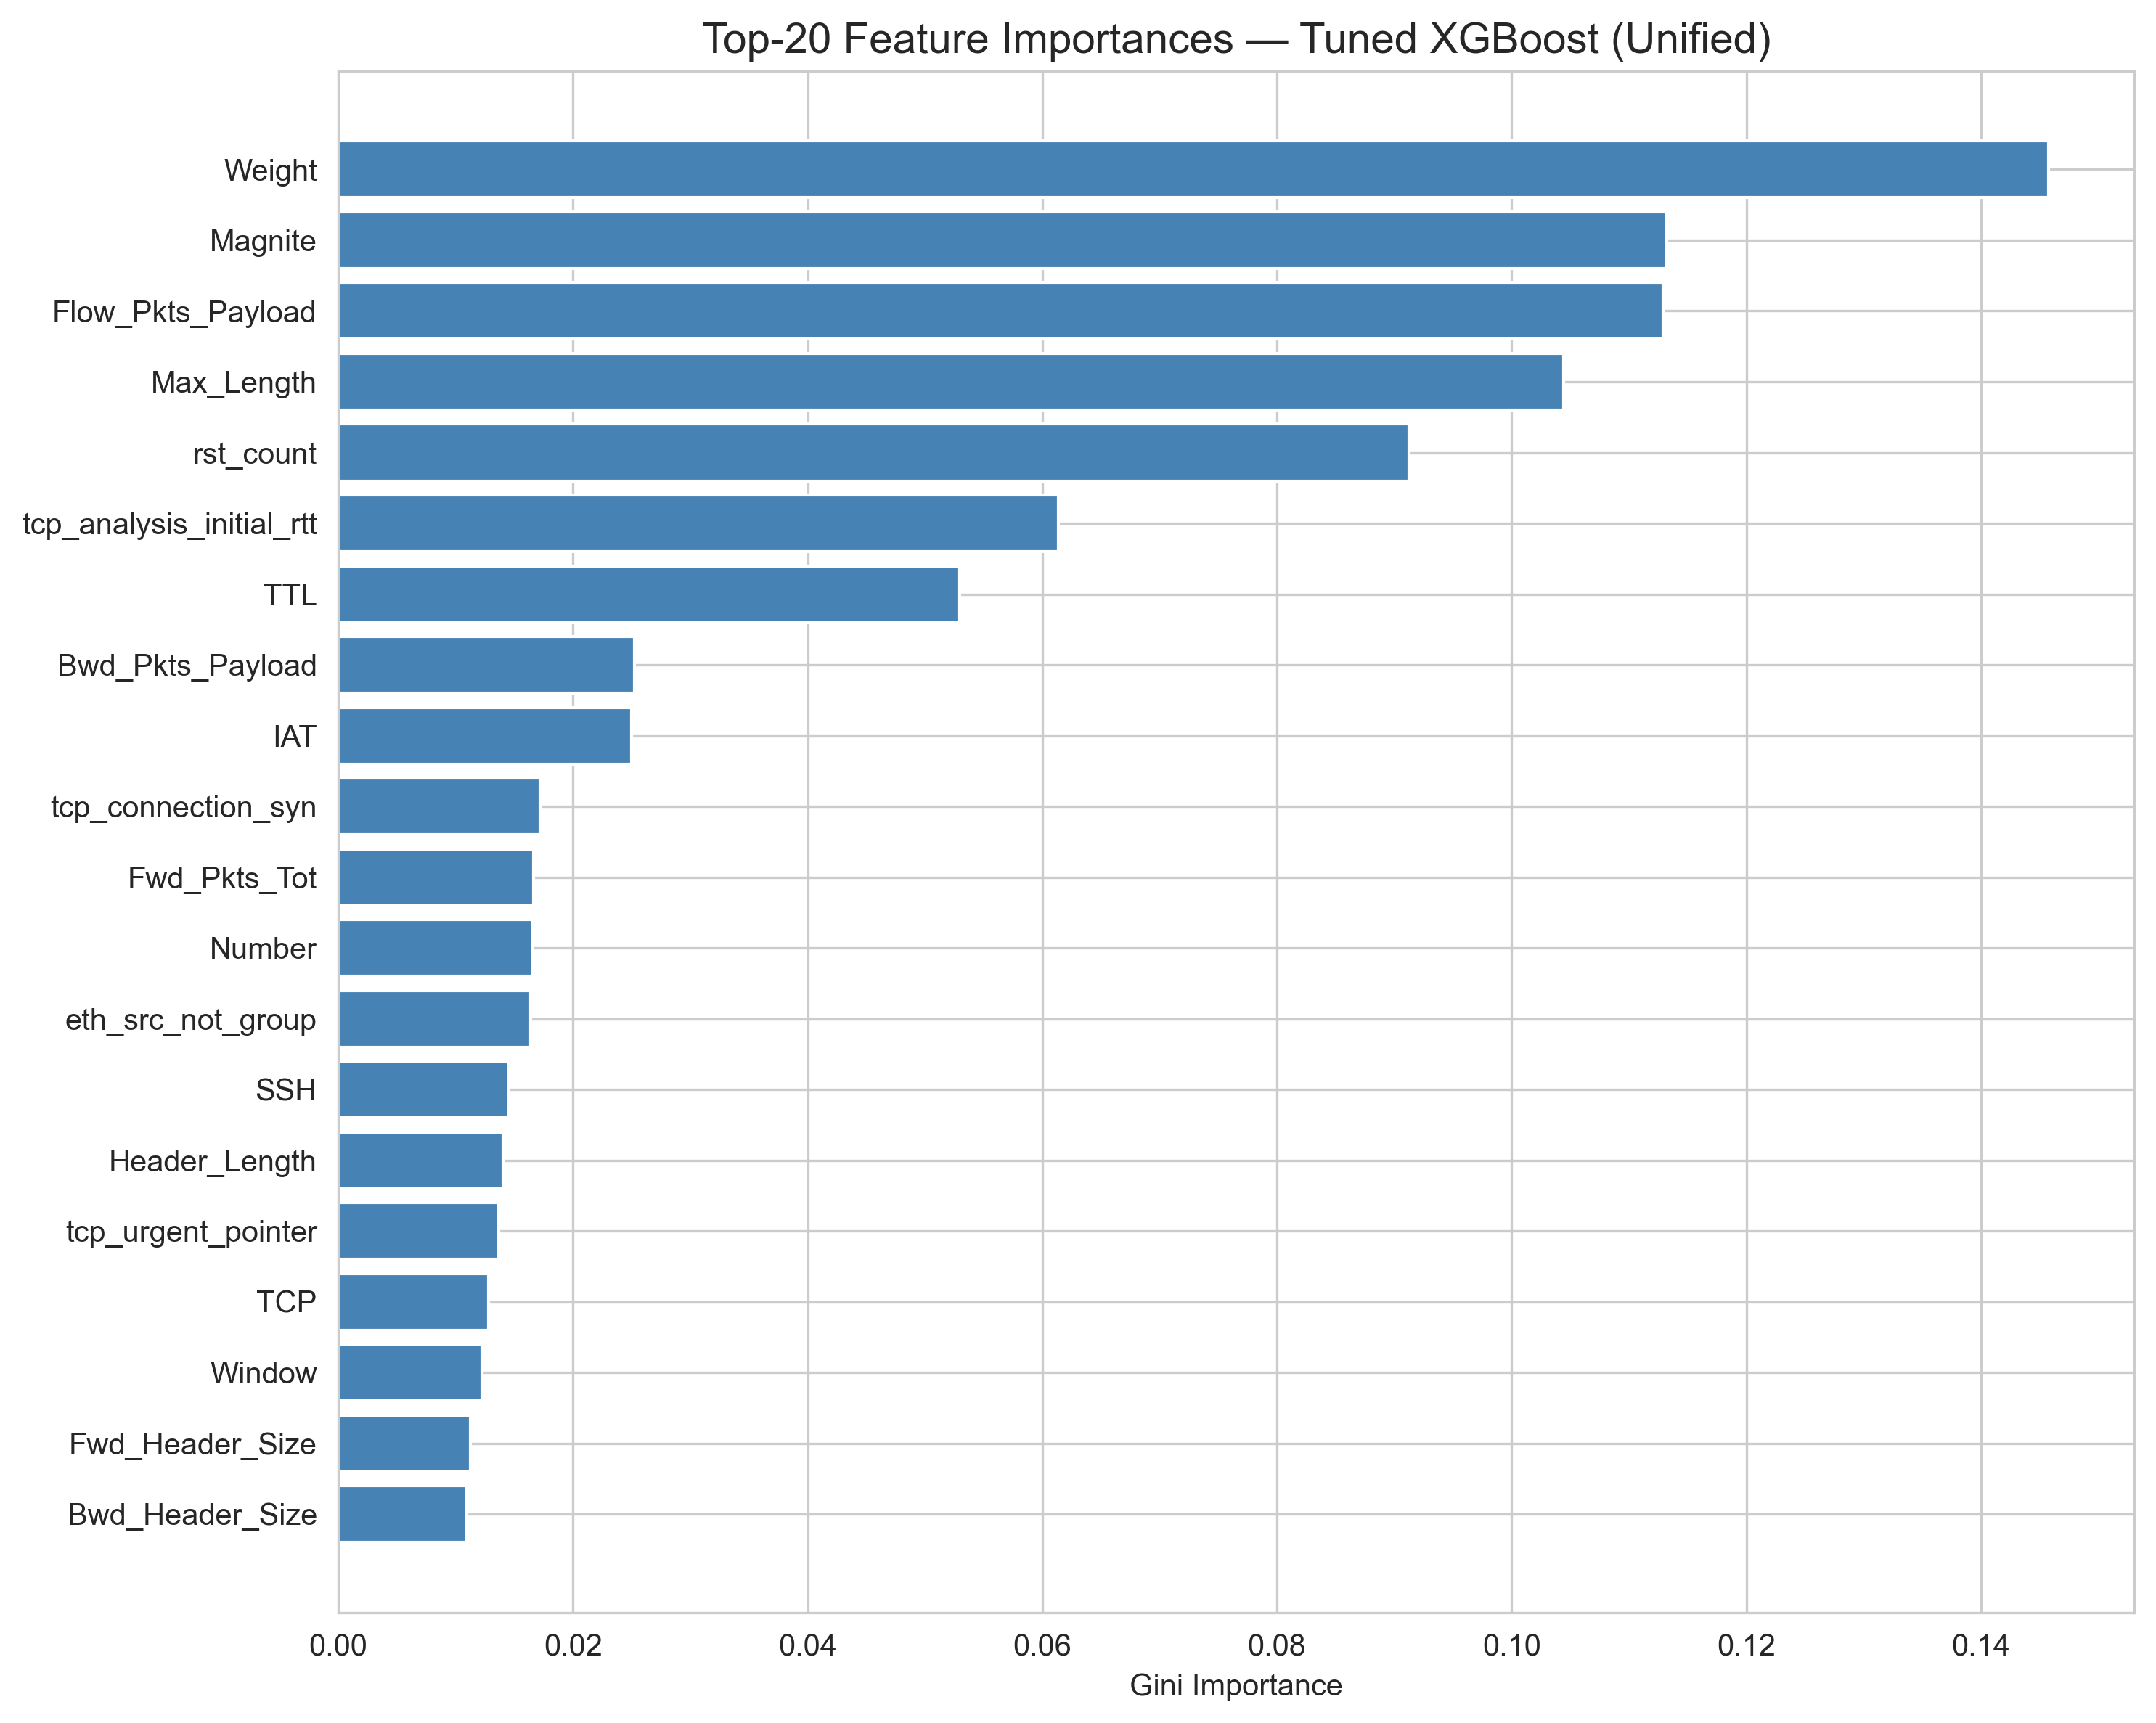
\includegraphics[width=0.85\textwidth]{ch5_xgb_feature_importance_unified.png}
\caption{Top-20 feature importances for the tuned XGBoost (Unified regime).}
\label{fig:xgb-feature-importance}
\end{figure}

\begin{figure}[H]
\centering
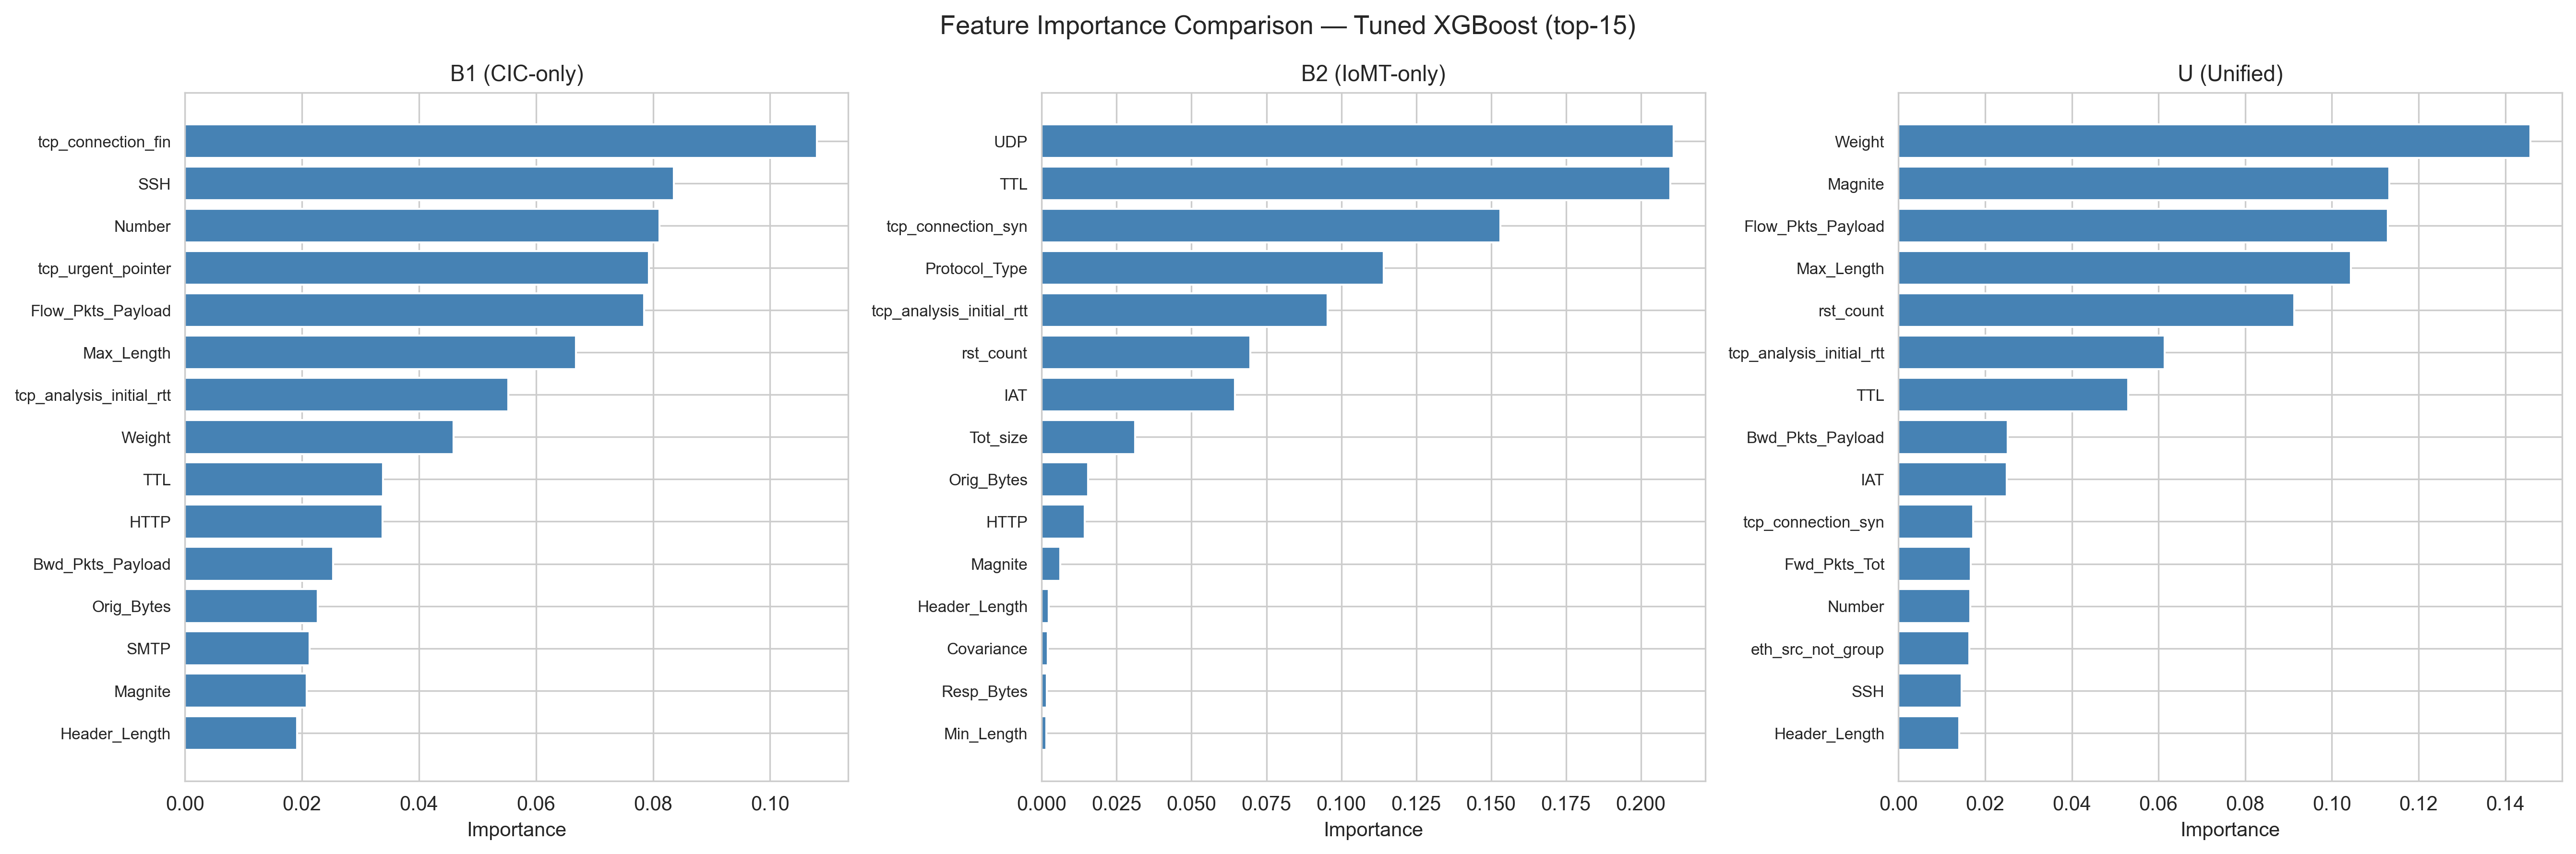
\includegraphics[width=\textwidth]{ch5_xgb_feature_importance_comparison.png}
\caption{Feature importance comparison across regimes (tuned XGBoost, top-15).}
\label{fig:xgb-fi-comparison}
\end{figure}

\subsubsection{Per-Class Analysis}

Figure~\ref{fig:xgb-per-class-f1} compares per-class F1 across tuned regimes on the full test set. Table~\ref{tab:xgb-perclass-unified} presents the detailed classification report for the Tuned U model.

\begin{figure}[H]
\centering
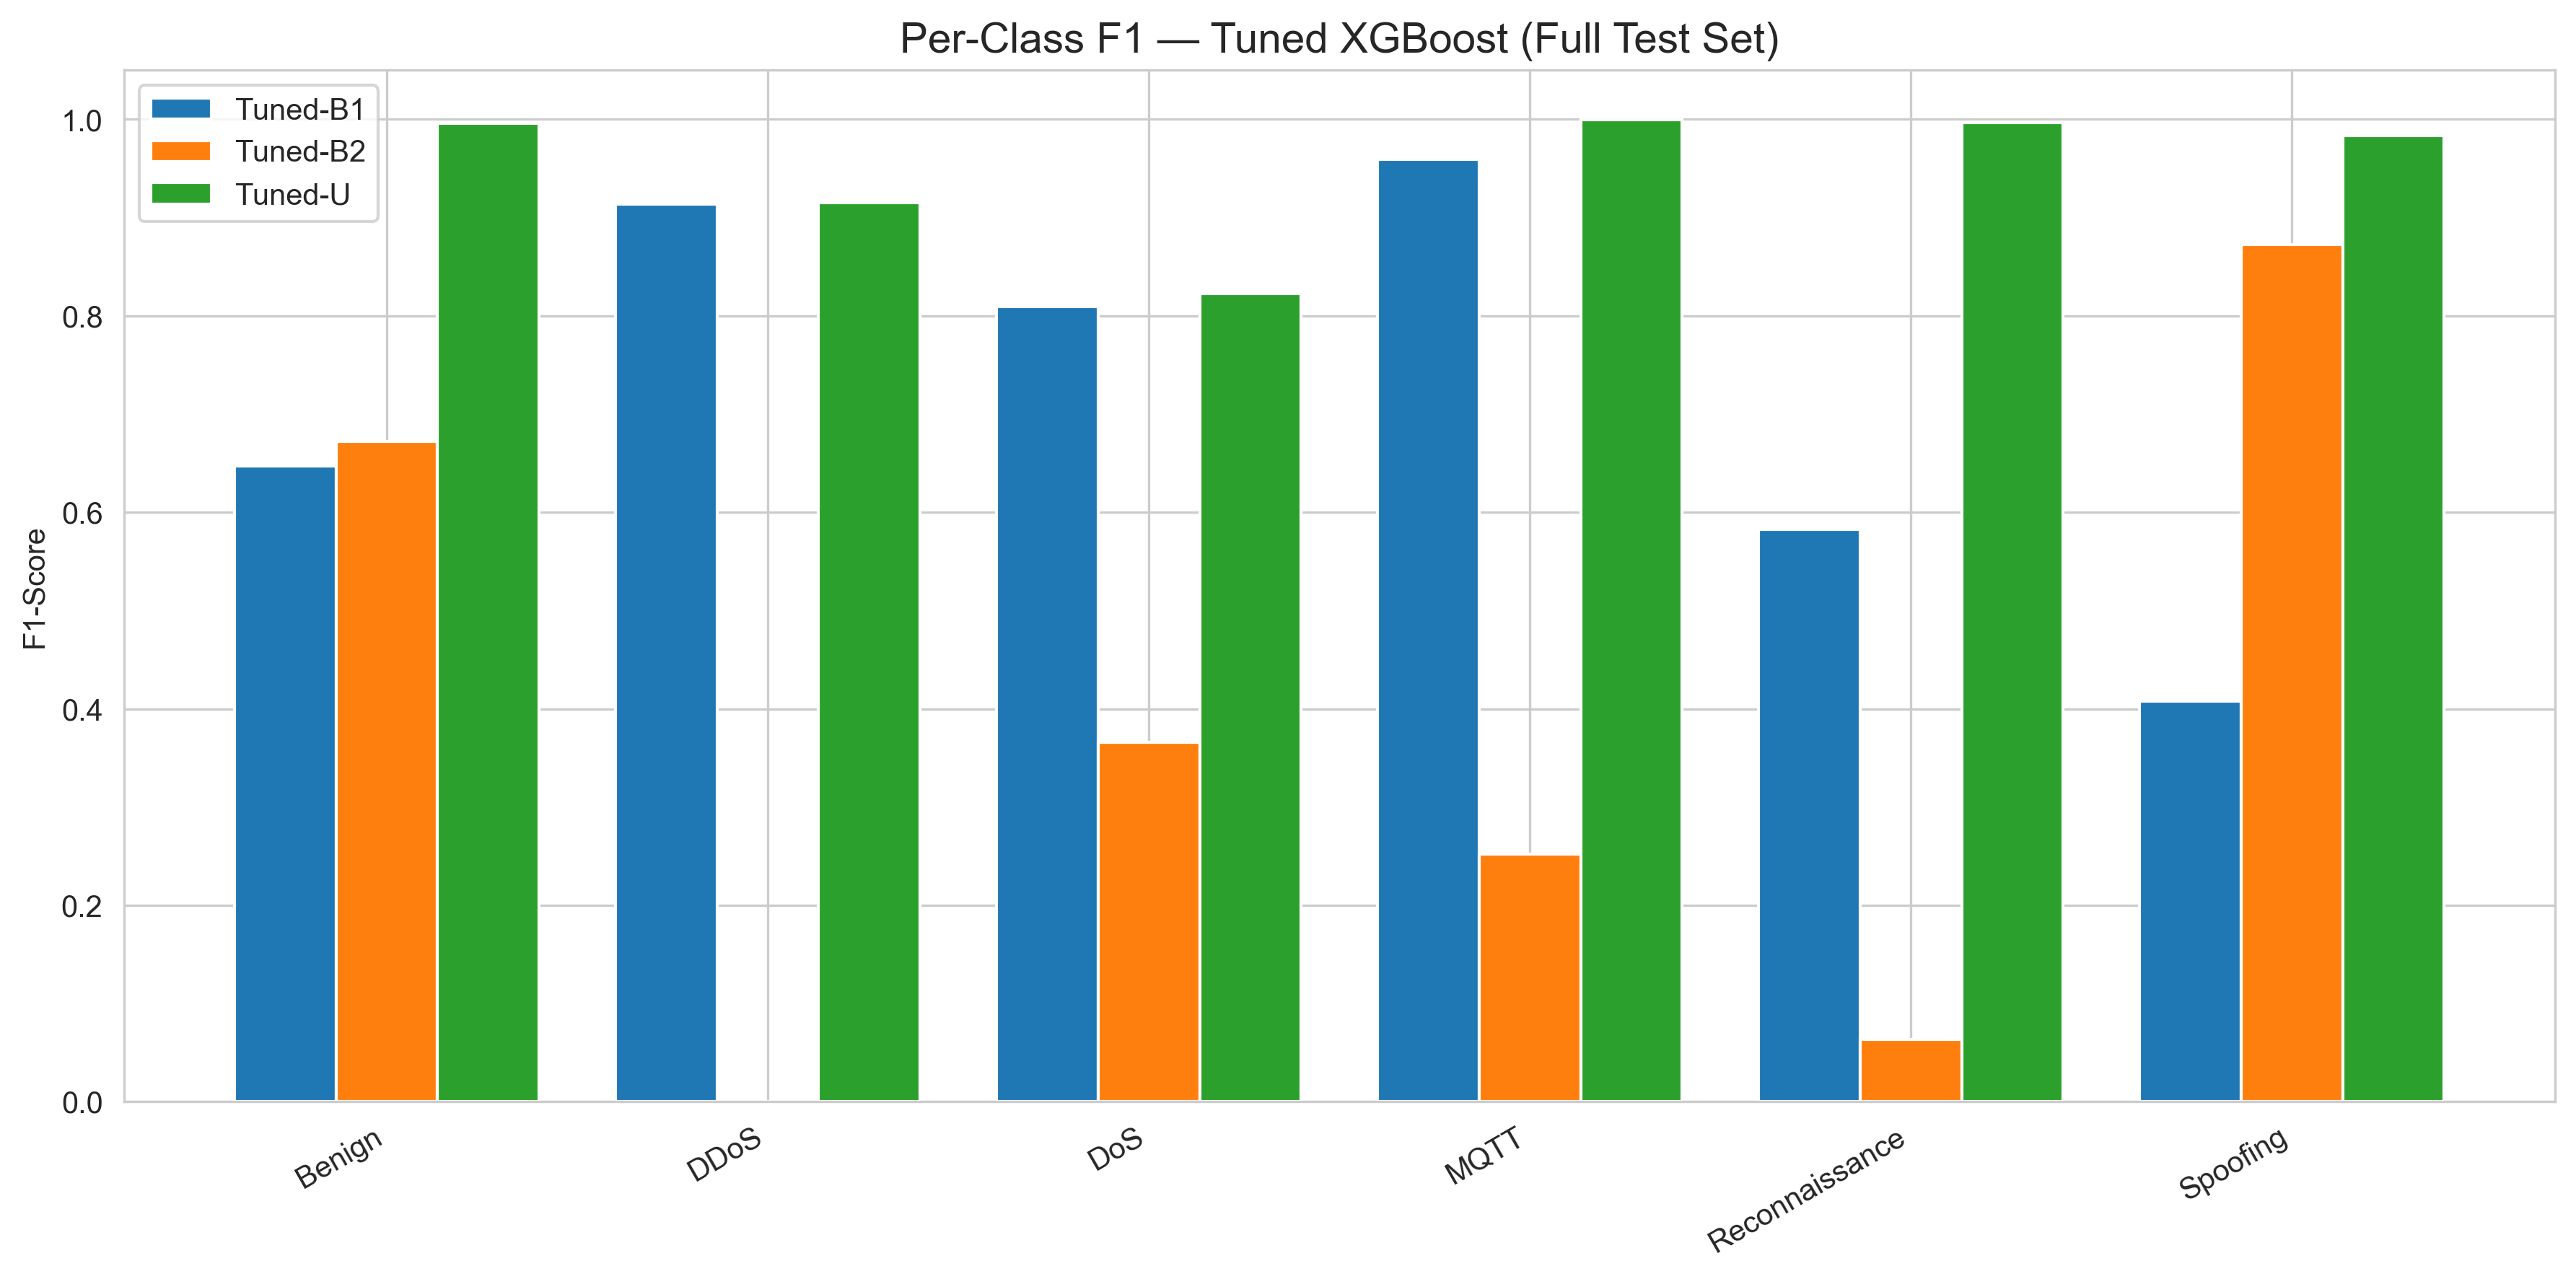
\includegraphics[width=0.85\textwidth]{ch5_xgb_per_class_f1.png}
\caption{Per-class F1-score comparison across regimes (tuned XGBoost, full test set).}
\label{fig:xgb-per-class-f1}
\end{figure}

\begin{table}[H]
\centering
\caption{Per-class classification report for the tuned unified XGBoost on the full test set (1,201,731 samples).}
\label{tab:xgb-perclass-unified}
\small
\begin{tabular}{@{}l r r r r@{}}
\toprule
\textbf{Class} & \textbf{Precision} & \textbf{Recall} & \textbf{F1-Score} & \textbf{Support} \\
\midrule
Benign          & 0.99 & 1.00 & 1.00 &     8,018 \\
DDoS            & 0.97 & 0.87 & 0.92 &   805,244 \\
DoS             & 0.74 & 0.93 & 0.82 &   322,273 \\
MQTT            & 1.00 & 1.00 & 1.00 &    57,891 \\
Reconnaissance  & 1.00 & 1.00 & 1.00 &     6,904 \\
Spoofing        & 0.98 & 0.99 & 0.98 &     1,401 \\
\midrule
Accuracy        &      &      & 0.89 & 1,201,731 \\
Macro avg       & 0.95 & 0.96 & 0.95 & 1,201,731 \\
Weighted avg    & 0.91 & 0.89 & 0.90 & 1,201,731 \\
\bottomrule
\end{tabular}
\end{table}

The tuned XGBoost unified model achieves the highest full-test Macro-F1 among the three classifiers (0.9522). The qualitative structure remains consistent with DT and RF: near-perfect scores on Benign (1.00), MQTT (1.00), Reconnaissance (1.00), and Spoofing (0.98), with residual error concentrated in the DDoS/DoS boundary. Relative to the tuned RF, XGBoost yields a marginal improvement in DDoS recall (0.87 vs.\ 0.86) and DoS precision (0.74 vs.\ 0.73), but DoS F1 remains 0.82 across all three models. The hypothesis that iterative residual learning would capture finer DDoS/DoS distinctions is therefore only very partially supported: gradient boosting provides a slight improvement in DDoS detection (F1: 0.91 $\to$ 0.92) but does not qualitatively resolve the boundary confusion, again confirming a feature-representation ceiling rather than a model-capacity limitation.

\subsubsection{Summary}

\begin{itemize}[nosep]
  \item \textbf{Strong unified performance.} Tuned U reaches Macro-F1 $=0.9522$ on the full test set, marginally above Random Forest (0.9487) and Decision Tree (0.9480).
  \item \textbf{B1 full-test dip after aggressive tuning.} Tuned B1's full Macro-F1 (0.7199) is lower than its baseline (0.7629), suggesting some hyperparameter combinations overfit the 300k-row search subsample relative to the full CIC-only training distribution---an acceptable trade-off given that the thesis focus is the unified regime, but worth monitoring in future work.
  \item \textbf{B2 behaviour unchanged at a high level.} In-domain IoMT Macro-F1 remains $\approx0.83$ while CIC/full slices stay poor, reflecting the missing DDoS class rather than the booster family.
  \item \textbf{DDoS/DoS boundary: marginal improvement only.} The hypothesis that gradient boosting's iterative residual learning would substantially improve the DDoS$\leftrightarrow$DoS separation is only very partially supported. DDoS F1 rises from 0.91 (DT, RF) to 0.92 (XGBoost); DoS F1 is unchanged at 0.82 across all three classifiers. This consistent plateau confirms that the DDoS/DoS confusion is a feature-representation constraint that cannot be resolved by increasing model complexity alone within the current 58-feature window space.
\end{itemize}

\subsection{Model Comparison}
\label{subsec:model-comparison}

Table~\ref{tab:model-compare-f1m} summarizes the primary metric (full-test Macro-F1) for the \emph{tuned} models under each training regime.

\begin{table}[H]
\centering
\caption{Full-test Macro-F1 (\textbf{primary metric}) for tuned classifiers.}
\label{tab:model-compare-f1m}
\small
\begin{tabular}{@{}l c c c@{}}
\toprule
\textbf{Classifier} & \textbf{B1 (CIC-only)} & \textbf{B2 (IoMT-only)} & \textbf{U (Unified)} \\
\midrule
Decision Tree  & 0.6959 & 0.3284 & 0.9480 \\
Random Forest  & 0.7395 & 0.2029 & 0.9487 \\
XGBoost        & 0.7199 & 0.3708 & \textbf{0.9522} \\
\bottomrule
\end{tabular}
\end{table}

\begin{table}[H]
\centering
\caption{Tuned unified (\textbf{U}) models: Macro-F1 on CIC-only, IoMT-only, and full test slices (values recomputed from stored \texttt{eval\_results.joblib} predictions).}
\label{tab:tuned-u-cross-slice-macrof1-present}
\small
\begin{tabular}{@{}l c c c@{}}
\toprule
\textbf{Classifier} & \textbf{CIC slice} & \textbf{IoMT slice} & \textbf{Full test} \\
\midrule
Decision Tree  & 0.9262 & 0.9990\textsuperscript{*} & 0.9480 \\
Random Forest  & 0.9285 & 0.9995\textsuperscript{*} & 0.9487 \\
XGBoost        & 0.9382 & 0.9999\textsuperscript{*} & 0.9522 \\
\bottomrule
\end{tabular}

\vspace{0.35em}
\raggedright\footnotesize
\textsuperscript{*}\,IoMT slice: Macro-F1 averaged over the five categories with non-zero ground-truth support (Benign, DoS, MQTT, Reconnaissance, Spoofing). The DDoS class has no IoMT test labels; excluding it from the macro average yields the values above. The \emph{global} six-class Macro-F1 on the same slice---still averaging over an empty DDoS column scored as F1\,=\,0---is $\approx$\,0.8325 (DT), $\approx$\,0.8329 (RF), and $\approx$\,0.8333 (XGB), which is why Tables~\ref{tab:dt-tuned}, \ref{tab:rf-tuned}, and~\ref{tab:xgb-tuned} retain the original reporting convention for strict cross-slice comparability.
\end{table}

Unified training consistently dominates: all three algorithms exceed 0.94 Macro-F1 on the full test when trained on U, whereas single-source regimes remain weak on the full mixture (especially B2, which never observes DDoS during training). Among algorithms, XGBoost edges out Random Forest and Decision Tree on the unified full test in this experiment, while Random Forest achieves the strongest B1-only full-test score---highlighting that ``best algorithm'' can depend on the deployment slice if one were forced to train single-source.

\subsection{Generalization to Real Hospital Traffic: HospNet26 Evaluation}
\label{subsec:hospnet26}

The evaluations presented in Sections~\ref{subsec:decision-tree}--\ref{subsec:model-comparison} are performed on test slices drawn from the same two laboratory datasets (CICIoMT2024 and IoMT-TrafficData) used for training. A more demanding generalization test is to apply the models to \emph{real} hospital network traffic that was captured in a live clinical environment and was not seen during any phase of training or tuning.

\paragraph{Dataset.}
HospNet26~\cite{hospnet26} is a publicly available reference dataset of anonymized network traffic features captured from the internal network of a Helios hospital (Germany) over one week (August 2025). Four \texttt{.parquet} files contain \emph{combined features}---72-column records integrating both flow-level and window-based (100-packet window) statistics---for four temporal segments: Friday, Weekend, Monday, and Monday-to-Friday. All 58 MIOTTA window-based features used by our models are present in these combined files as a strict subset of the 72 available columns; the 14 additional flow-level columns are discarded. The dataset contains \textbf{no attack labels}: every record represents a traffic window observed in the live hospital network and is presumed benign.

\paragraph{Processing protocol.}
To ensure a fair and consistent comparison with the preceding experiments, the following steps exactly mirror the training-time preprocessing pipeline:
\begin{enumerate}[nosep]
  \item The four temporal files are concatenated into a single dataset of \textbf{1,265,240 windows}.
  \item The 58 features are extracted in the same column order as the training feature matrix.
  \item The same \texttt{StandardScaler} fitted on the \emph{training} split of the unified dataset is applied (no refitting on HospNet26 data, which would constitute data leakage).
  \item Predictions are obtained from the three tuned Unified models (DT-U, RF-U, XGB-U) without any retraining.
\end{enumerate}

\paragraph{Evaluation metric.}
Since no ground-truth labels exist, standard classification metrics (Macro-F1, accuracy) cannot be computed. The appropriate metric is the \textbf{Benign prediction rate}---the fraction of windows that each model classifies as \texttt{Benign}---which measures the model's \emph{specificity} on unseen real-world traffic. A high rate indicates that the model does not generate false alarms on legitimate hospital traffic; a low rate signals a distributional gap between the training-set ``benign'' traffic and real clinical network activity.

\begin{table}[H]
\centering
\caption{HospNet26 generalization evaluation: prediction distribution for the three tuned Unified models on 1,265,240 unlabelled real hospital traffic windows. All windows are presumed benign; the Benign prediction rate is the specificity proxy; all other predicted classes are false positives.}
\label{tab:hospnet26-eval}
\small
\begin{tabular}{@{}l r r r r r r | r@{}}
\toprule
\textbf{Model} & \textbf{Benign} & \textbf{DDoS} & \textbf{DoS} & \textbf{MQTT} & \textbf{Recon.} & \textbf{Spoofing} & \textbf{Benign rate} \\
\midrule
Decision Tree  & 6.07\% &  7.80\% & 72.04\% & 0.22\% &  5.30\% &  8.57\% & \textbf{6.07\%} \\
Random Forest  & 3.72\% &  0.60\% & 71.37\% & 0.06\% & 19.08\% &  5.17\% & \textbf{3.72\%} \\
XGBoost        & 9.96\% & 23.80\% & 51.14\% & 0.11\% &  4.28\% & 10.71\% & \textbf{9.96\%} \\
\bottomrule
\end{tabular}
\end{table}
\FloatBarrier

\paragraph{Results and interpretation.}
All three models classify between 90\% and 96\% of real hospital traffic windows as some form of attack, yielding Benign prediction rates of only 3.7\%--10.0\%. This result is \textbf{expected and interpretable} given the following factors.

\begin{enumerate}[nosep]
  \item \textbf{Training-set benign traffic is not representative of real clinical environments.} The ``Benign'' class in CICIoMT2024 and IoMT-TrafficData was generated in controlled laboratory or emulated testbed conditions. Real hospital networks carry a fundamentally different traffic mix: medical imaging (DICOM/PACS), electronic health record systems (HL7, FHIR), proprietary clinical device protocols, and large-scale background administrative traffic. The window-based statistical signatures of these flows (packet rates, byte distributions, IAT patterns) fall outside the distributional support learned by the classifier for the Benign class.

  \item \textbf{The dominant false-positive class is DoS.} Across all three models, 51--72\% of hospital windows are predicted as DoS. This is consistent with the hypothesis that high-throughput clinical data transfers (e.g., continuous PACS image streaming or bulk EMR synchronization) produce burst-like packet statistics that overlap with the DoS feature region. These traffic patterns generate high values of flow-rate and window-size features, which the models have learned to associate with volumetric denial-of-service attacks.

  \item \textbf{Specificity varies across models.} XGBoost achieves the highest Benign prediction rate (9.96\%) and the most distributed false-positive profile. Decision Tree and Random Forest concentrate errors more heavily in the DoS region, consistent with their simpler decision boundaries. The week-day temporal pattern is also notable: Weekend windows show markedly lower Benign rates (0.86\%--5.86\%) than weekday segments, suggesting that reduced administrative traffic during weekends creates statistical profiles even further from the training-set Benign distribution.

  \item \textbf{This is a distributional-shift finding, not a model failure.} The models achieve Macro-F1 $\geq 0.948$ on the laboratory test set. The sharp drop in specificity on HospNet26 is attributable to the \emph{covariate shift} between synthetic/emulated benign traffic and live clinical traffic---a fundamental limitation of training on laboratory datasets that has been widely documented in the IDS literature~\cite{sommer2010outside}. Closing this gap would require either retraining with representative samples of real hospital benign traffic, or applying domain-adaptation techniques, both of which are natural directions for future work.
\end{enumerate}

\paragraph{Toward closing the gap: a recalibration strategy.}
The results above suggest a concrete actionable path for future deployment. Because the models already achieve near-perfect separation of \emph{attack} categories (Macro-F1 $\geq 0.948$ on laboratory data), the remaining challenge is not detection capability but \emph{Benign-class recalibration}: the models need to learn what normal traffic looks like in the target environment. Two complementary strategies are proposed:

\begin{enumerate}[nosep]
  \item \textbf{Few-shot Benign fine-tuning.} A small, representative sample of confirmed-benign traffic from the target hospital network (e.g., a supervised collection of $\sim$10{,}000--50{,}000 windows over one business day) would be added to the training set with the Benign label. The model is then retrained (or fine-tuned) on the augmented dataset. This approach preserves all attack-detection capability while shifting the Benign decision boundary to encompass real clinical traffic patterns. The required collection effort is modest: HospNet26 demonstrates that a single week of capture already yields over 1.2 million windows.

  \item \textbf{Threshold-based post-hoc calibration.} Instead of retraining, probability outputs from the existing models (e.g., XGBoost's \texttt{predict\_proba}) can be recalibrated using a held-out set of known-benign hospital windows. A class-specific decision threshold is then optimized to trade off false-positive rate against detection sensitivity, targeting the operational requirements of the clinical environment (e.g., an acceptable false-alarm rate of $\leq 1$\%).
\end{enumerate}

Both strategies are designed to be low-cost and operationally feasible: they require only benign traffic samples (which are abundant in any live network) and do not demand labelled attack data from the hospital, which would be ethically and practically difficult to obtain.

In summary, the HospNet26 evaluation reveals a critical open challenge: the unified models, despite strong performance on held-out laboratory data, are not yet ready for zero-shot deployment in a real clinical network without a benign-traffic recalibration step. This finding strengthens the thesis argument that dataset diversity must encompass \emph{real} deployment environments, not only multi-source laboratory collections, and provides a clear, actionable research direction for bridging the laboratory-to-clinic gap.

\subsection{Discussion of Results}
\label{subsec:discussion}

The experiments in Section~\ref{sec:model-evaluation} support two main conclusions. First, \textbf{multi-source integration (regime U) is the decisive factor} for high Macro-F1 and balanced cross-domain behaviour on the unified test set: class-weighted tree models of increasing complexity all benefit from seeing both CIC-style and IoMT-style traffic during training. Second, \textbf{within the unified regime, moderate complexity gains are incremental}: Decision Tree $\to$ Random Forest $\to$ XGBoost improves full-test Macro-F1 from 0.9480 to 0.9522---meaningful but smaller than the $\approx$0.20--0.75 swing induced by switching from single-source to unified training. The persistent DDoS/DoS confusion across all three families indicates a \emph{feature-representation} limitation (window statistics without explicit multi-source diversity) more than a \emph{model-capacity} ceiling.

\paragraph{Statistical significance of pairwise model comparisons (McNemar's test).}
Following the recommendation of Lones~\cite{lones2024avoid}, statistical significance of the classifier differences is assessed with \textbf{McNemar's test}~\cite{mcnemar1947note}, which is designed for paired observations on the same test set. For each pair of tuned Unified models, the contingency table records $b$ (samples where model~A is correct and model~B is wrong) and $c$ (samples where model~A is wrong and model~B is correct); the test statistic with Yates' continuity correction is $\chi^2 = (|b-c|-1)^2\,/\,(b+c)$, evaluated against $\chi^2_1$.

Table~\ref{tab:mcnemar} reports the results. The \emph{relative error reduction} (RER) $= (e_A - e_B)/e_A \times 100$ provides the effect-size complement, since with $N=1{,}201{,}731$ test samples even trivially small differences yield $p \ll 0.001$.

\begin{table}[H]
\centering
\caption{McNemar's test results for pairwise comparison of tuned Unified models on the full test set ($N=1{,}201{,}731$). $b$: model~A correct, model~B wrong; $c$: model~A wrong, model~B correct; RER: relative error reduction A~$\to$~B (positive $=$ B better).}
\label{tab:mcnemar}
\small
\begin{tabular}{@{}l c c r r c@{}}
\toprule
\textbf{Pair (A vs B)} & $b$ & $c$ & $\chi^2$ (Yates) & $p$-value & \textbf{RER (\%)} \\
\midrule
DT vs RF  & 6,919 & 6,372 & 22.43 & $2.2 \times 10^{-6}$ & $-0.41$ \\
DT vs XGB & 7,314 & 11,297 & 851.99 & $< 10^{-15}$ & $+2.98$ \\
RF vs XGB & 4,246 & 8,776 & 1{,}575.17 & $< 10^{-15}$ & $+3.38$ \\
\bottomrule
\end{tabular}
\end{table}
\FloatBarrier

Three observations deserve emphasis.

\begin{enumerate}[nosep]
  \item \textbf{XGBoost vs DT and RF are statistically and practically significant.} Both comparisons yield $\chi^2 > 850$ with $p < 10^{-15}$ and a relative error reduction of approximately 3\%, confirming that XGBoost's advantage is not a sampling artefact.
  \item \textbf{DT vs RF: statistically significant, but the direction is counter-intuitive.} Although RF achieves a higher Macro-F1 than DT (0.9487 vs 0.9480), it actually makes \emph{more} total errors (134,071 vs 133,524), resulting in a negative RER of $-0.41$\%. This apparent contradiction is resolved by recognising that Macro-F1 weights each class equally: RF redistributes its errors away from minority classes (Benign, Reconnaissance, Spoofing) toward the majority class (DDoS/DoS boundary), which penalises overall accuracy but improves the per-class average. This is precisely the behaviour intended by the balanced-class-weight protocol, and it illustrates why Macro-F1 is the appropriate primary metric for this imbalanced dataset.
  \item \textbf{Large-sample caveat.} With $N > 10^6$, McNemar's test detects statistically significant differences even when the practical effect is negligible. The RER column should therefore be consulted alongside the $p$-value. A RER of $-0.41$\% (DT vs RF) represents approximately 547 fewer correct predictions per model out of 1.2 million---a marginal real-world difference.
\end{enumerate}

\paragraph{Hyperparameter optimisation beyond RandomizedSearchCV.}
This thesis deliberately uses \texttt{RandomizedSearchCV} with a fixed iteration budget for all models to preserve methodological comparability. In industrial pipelines, \textbf{Bayesian optimisation} (e.g.\ Optuna with the Tree-structured Parzen Estimator) or multi-fidelity schedulers (Hyperband, BOHB) can often reach equal or better validation scores with fewer expensive full-data evaluations, especially when combined with early pruning of unpromising trials. Adopting such tools is a natural extension for future work, provided the same outer train/validation/test discipline is maintained.

% ══════════════════════════════════════════════════════════════════════════════
\section{Answering the Research Question}
\label{sec:answering-rq}

This section synthesizes how the integration methodology and empirical results (Section~\ref{sec:model-evaluation}) address the research question: \textit{``How can the integration of multiple heterogeneous datasets improve the performance and generalizability of a machine learning model in detecting intrusions in IoMT environments?''} It is placed after model training and evaluation so that claims are grounded in measured outcomes.

\subsection{How Integration Was Achieved}
\label{subsec:how-integration}

Three technical decisions form the backbone of the integration methodology:

\begin{enumerate}[nosep]
  \item \textbf{MIOTTA-NPT as the feature-unification enabler.}
  Both source datasets were processed through the same tool (MIOTTA-NPT in \emph{combined} mode, window size $=100$ packets), yielding an identical 58-column numeric feature space without manual feature engineering. This eliminates the feature-heterogeneity barrier (Problem~P2, Section~\ref{sec:problem}): because all statistical windows share the same column semantics regardless of origin, concatenation is structurally valid by construction.

  \item \textbf{Three-level label harmonization.}
  A hierarchical label scheme was designed with three granularity tiers: binary (\texttt{Benign}/\texttt{Attack}), categorical (six attack families: Benign, DDoS, DoS, MQTT, Reconnaissance, Spoofing), and fine-grained (original attack labels). The categorical tier resolves the label-inconsistency problem (P3) by mapping divergent naming conventions (e.g., \texttt{DDoS\_TCP\_Flood} and \texttt{TCP\_DDoS}) to a shared taxonomy, while preserving the original fine-grained labels for future research requiring higher specificity.

  \item \textbf{Source attribution and stratified splitting.}
  Each record retains its \texttt{source\_dataset} provenance, enabling the three-regime evaluation design (B1, B2, U) that isolates the effect of integration from the effect of model choice. Stratified splits are performed \emph{before} regime filtering, guaranteeing that all regimes share the same test partition boundaries and that cross-domain comparisons are methodologically valid.
\end{enumerate}

\subsection{Evidence of Improved Generalizability}
\label{subsec:improved-coverage}

The experimental evidence supports three concrete claims regarding the benefit of multi-source integration:

\paragraph{Claim 1: Unified training resolves the cross-domain collapse.}
Single-source models exhibit catastrophic cross-domain failure: the best single-source Macro-F1 on the opposite source's test slice is 0.34 (B1$\to$IoMT, RF) and 0.11 (B2$\to$CIC, XGB). Unified models, by contrast, achieve Macro-F1 $\geq 0.93$ on \emph{both} CIC-only and IoMT-only slices simultaneously (Table~\ref{tab:tuned-u-cross-slice-macrof1-present}), confirming that integration transforms the feature space from source-specific into source-agnostic.

\paragraph{Claim 2: Unified training is the dominant factor; model complexity is secondary.}
Within the unified regime, the Macro-F1 improvement from DT to XGBoost is +0.42 percentage points (0.9480 $\to$ 0.9522). Switching from the best single-source model (B1-RF, 0.7395) to the weakest unified model (U-DT, 0.9480) produces a +20.85 percentage-point jump. The contribution of integration is therefore \textbf{50$\times$ larger} than the contribution of model complexity, directly answering the research question: dataset integration is the primary lever for improving generalizability.

\paragraph{Claim 3: A residual generalization gap persists toward real clinical environments.}
The HospNet26 evaluation (Section~\ref{subsec:hospnet26}) reveals that Benign prediction rates on real hospital traffic range from 3.7\% to 10.0\%, indicating that even unified multi-source training on laboratory datasets does not close the distributional gap to live clinical networks. This finding qualifies the positive answer to the research question: integration of \emph{laboratory} sources improves cross-domain generalization \emph{among those sources}, but deployment-level generalizability requires incorporating representative samples from the target operational environment---a direction explored in Section~\ref{subsec:hospnet26} and elaborated in the future-work discussion (Chapter~\ref{ch:conclusions}).

% ══════════════════════════════════════════════════════════════════════════════
\section{Chapter Summary}
\label{sec:experimentation-summary}

This chapter presented the empirical evaluation of the unified dataset across five complementary dimensions:

\begin{enumerate}[nosep]
  \item \textbf{Structural integrity} (Section~\ref{sec:quality-assessment}): The 8-million-record dataset was verified for completeness, type consistency, feature scaling, label coherence, and split-boundary integrity, with zero defects found.

  \item \textbf{Model training and tuning} (Sections~\ref{subsec:decision-tree}--\ref{subsec:xgboost}): Three tree-based classifiers of increasing complexity (DT, RF, XGBoost) were trained and tuned under three regimes (CIC-only, IoMT-only, Unified), producing 18 models with a strict ``test set once'' protocol and identical tuning budgets.

  \item \textbf{Cross-domain and per-class analysis}: The unified regime (U) consistently dominated both single-source baselines, achieving Macro-F1 of 0.9480 (DT), 0.9487 (RF), and 0.9522 (XGBoost) on the full test set. The DDoS/DoS confusion boundary was identified as a persistent feature-representation limitation, accounting for $>$99\% of all errors across all three models.

  \item \textbf{Real-world generalization} (Section~\ref{subsec:hospnet26}): Deploying the models on 1.26 million unlabelled windows from a real German hospital network (HospNet26) revealed a sharp specificity drop (Benign rate 3.7--10.0\%), quantifying the covariate shift between laboratory and clinical traffic and motivating domain-adaptation as a priority for future work.

  \item \textbf{Statistical significance} (Section~\ref{subsec:discussion}): McNemar's test confirmed that XGBoost's advantage over DT and RF is both statistically significant and practically meaningful ($\approx$3\% relative error reduction), while the DT-vs-RF difference, though statistically significant, is practically marginal.
\end{enumerate}

Together, these results provide a comprehensive answer to the research question: multi-source integration is the decisive factor for improving IDS generalizability across laboratory IoMT environments, while closing the residual gap to real clinical networks remains an open challenge requiring targeted data collection.
